% Options for packages loaded elsewhere
\PassOptionsToPackage{unicode}{hyperref}
\PassOptionsToPackage{hyphens}{url}
%
\documentclass[
  11pt,
  letterpaper,
]{scrbook}

\usepackage{amsmath,amssymb}
\usepackage{lmodern}
\usepackage{iftex}
\ifPDFTeX
  \usepackage[T1]{fontenc}
  \usepackage[utf8]{inputenc}
  \usepackage{textcomp} % provide euro and other symbols
\else % if luatex or xetex
  \usepackage{unicode-math}
  \defaultfontfeatures{Scale=MatchLowercase}
  \defaultfontfeatures[\rmfamily]{Ligatures=TeX,Scale=1}
\fi
% Use upquote if available, for straight quotes in verbatim environments
\IfFileExists{upquote.sty}{\usepackage{upquote}}{}
\IfFileExists{microtype.sty}{% use microtype if available
  \usepackage[]{microtype}
  \UseMicrotypeSet[protrusion]{basicmath} % disable protrusion for tt fonts
}{}
\makeatletter
\@ifundefined{KOMAClassName}{% if non-KOMA class
  \IfFileExists{parskip.sty}{%
    \usepackage{parskip}
  }{% else
    \setlength{\parindent}{0pt}
    \setlength{\parskip}{6pt plus 2pt minus 1pt}}
}{% if KOMA class
  \KOMAoptions{parskip=half}}
\makeatother
\usepackage{xcolor}
\usepackage[top=1in,left=1in]{geometry}
\setlength{\emergencystretch}{3em} % prevent overfull lines
\setcounter{secnumdepth}{5}
% Make \paragraph and \subparagraph free-standing
\ifx\paragraph\undefined\else
  \let\oldparagraph\paragraph
  \renewcommand{\paragraph}[1]{\oldparagraph{#1}\mbox{}}
\fi
\ifx\subparagraph\undefined\else
  \let\oldsubparagraph\subparagraph
  \renewcommand{\subparagraph}[1]{\oldsubparagraph{#1}\mbox{}}
\fi


\providecommand{\tightlist}{%
  \setlength{\itemsep}{0pt}\setlength{\parskip}{0pt}}\usepackage{longtable,booktabs,array}
\usepackage{calc} % for calculating minipage widths
% Correct order of tables after \paragraph or \subparagraph
\usepackage{etoolbox}
\makeatletter
\patchcmd\longtable{\par}{\if@noskipsec\mbox{}\fi\par}{}{}
\makeatother
% Allow footnotes in longtable head/foot
\IfFileExists{footnotehyper.sty}{\usepackage{footnotehyper}}{\usepackage{footnote}}
\makesavenoteenv{longtable}
\usepackage{graphicx}
\makeatletter
\def\maxwidth{\ifdim\Gin@nat@width>\linewidth\linewidth\else\Gin@nat@width\fi}
\def\maxheight{\ifdim\Gin@nat@height>\textheight\textheight\else\Gin@nat@height\fi}
\makeatother
% Scale images if necessary, so that they will not overflow the page
% margins by default, and it is still possible to overwrite the defaults
% using explicit options in \includegraphics[width, height, ...]{}
\setkeys{Gin}{width=\maxwidth,height=\maxheight,keepaspectratio}
% Set default figure placement to htbp
\makeatletter
\def\fps@figure{htbp}
\makeatother
\newlength{\cslhangindent}
\setlength{\cslhangindent}{1.5em}
\newlength{\csllabelwidth}
\setlength{\csllabelwidth}{3em}
\newlength{\cslentryspacingunit} % times entry-spacing
\setlength{\cslentryspacingunit}{\parskip}
\newenvironment{CSLReferences}[2] % #1 hanging-ident, #2 entry spacing
 {% don't indent paragraphs
  \setlength{\parindent}{0pt}
  % turn on hanging indent if param 1 is 1
  \ifodd #1
  \let\oldpar\par
  \def\par{\hangindent=\cslhangindent\oldpar}
  \fi
  % set entry spacing
  \setlength{\parskip}{#2\cslentryspacingunit}
 }%
 {}
\usepackage{calc}
\newcommand{\CSLBlock}[1]{#1\hfill\break}
\newcommand{\CSLLeftMargin}[1]{\parbox[t]{\csllabelwidth}{#1}}
\newcommand{\CSLRightInline}[1]{\parbox[t]{\linewidth - \csllabelwidth}{#1}\break}
\newcommand{\CSLIndent}[1]{\hspace{\cslhangindent}#1}

\newcommand{\df}[1]{\frac{\partial}{\partial #1}}
\newcommand{\R}{\mathbf{R}}
\usepackage{listings}
\makeatletter
\makeatother
\makeatletter
\@ifpackageloaded{bookmark}{}{\usepackage{bookmark}}
\makeatother
\makeatletter
\@ifpackageloaded{caption}{}{\usepackage{caption}}
\AtBeginDocument{%
\ifdefined\contentsname
  \renewcommand*\contentsname{Table of contents}
\else
  \newcommand\contentsname{Table of contents}
\fi
\ifdefined\listfigurename
  \renewcommand*\listfigurename{List of Figures}
\else
  \newcommand\listfigurename{List of Figures}
\fi
\ifdefined\listtablename
  \renewcommand*\listtablename{List of Tables}
\else
  \newcommand\listtablename{List of Tables}
\fi
\ifdefined\figurename
  \renewcommand*\figurename{Figure}
\else
  \newcommand\figurename{Figure}
\fi
\ifdefined\tablename
  \renewcommand*\tablename{Table}
\else
  \newcommand\tablename{Table}
\fi
}
\@ifpackageloaded{float}{}{\usepackage{float}}
\floatstyle{ruled}
\@ifundefined{c@chapter}{\newfloat{codelisting}{h}{lop}}{\newfloat{codelisting}{h}{lop}[chapter]}
\floatname{codelisting}{Listing}
\newcommand*\listoflistings{\listof{codelisting}{List of Listings}}
\usepackage{amsthm}
\theoremstyle{plain}
\newtheorem{algorithm}{Algorithm}[chapter]
\theoremstyle{plain}
\newtheorem{theorem}{Theorem}[chapter]
\theoremstyle{remark}
\renewcommand*{\proofname}{Proof}
\newtheorem*{remark}{Remark}
\newtheorem*{solution}{Solution}
\makeatother
\makeatletter
\@ifpackageloaded{caption}{}{\usepackage{caption}}
\@ifpackageloaded{subcaption}{}{\usepackage{subcaption}}
\makeatother
\makeatletter
\@ifpackageloaded{tcolorbox}{}{\usepackage[many]{tcolorbox}}
\makeatother
\makeatletter
\@ifundefined{shadecolor}{\definecolor{shadecolor}{rgb}{.97, .97, .97}}
\makeatother
\makeatletter
\makeatother
\ifLuaTeX
  \usepackage{selnolig}  % disable illegal ligatures
\fi
\IfFileExists{bookmark.sty}{\usepackage{bookmark}}{\usepackage{hyperref}}
\IfFileExists{xurl.sty}{\usepackage{xurl}}{} % add URL line breaks if available
\urlstyle{same} % disable monospaced font for URLs
\hypersetup{
  pdftitle={Lectures on Machine Learning},
  pdfauthor={Jeremy Teitelbaum},
  hidelinks,
  pdfcreator={LaTeX via pandoc}}

\title{Lectures on Machine Learning}
\author{Jeremy Teitelbaum}
\date{12/1/22}

\begin{document}
\frontmatter
\maketitle
\ifdefined\Shaded\renewenvironment{Shaded}{\begin{tcolorbox}[breakable, boxrule=0pt, borderline west={3pt}{0pt}{shadecolor}, interior hidden, frame hidden, enhanced, sharp corners]}{\end{tcolorbox}}\fi

\renewcommand*\contentsname{Table of contents}
{
\setcounter{tocdepth}{2}
\tableofcontents
}
\mainmatter
\bookmarksetup{startatroot}

\hypertarget{preface}{%
\chapter*{Preface}\label{preface}}
\addcontentsline{toc}{chapter}{Preface}

\markboth{Preface}{Preface}

These notes are being developed for the UConn Math Department's
undergraduate course on the Mathematics of Machine Learning, Math 3180.

This is a (very) \emph{rough draft}.

You can
\href{https://github.com/jeremy9959/Mathematics-for-Machine-Learning}{view
this project on GitHub}. Please let the author know if you have
questions or find mistakes by opening an issue there.

\bookmarksetup{startatroot}

\hypertarget{sec-LinearRegression}{%
\chapter{Linear Regression}\label{sec-LinearRegression}}

\[\newcommand{\df}[1]{\frac{\partial}{\partial #1}}\]
\[\newcommand{\R}{\mathbf{R}}\] \#\# Introduction \{\#sec-Intro\}

Suppose that we are trying to study two quantities \(x\) and \(y\) that
we suspect are related -- at least approximately -- by a linear equation
\(y=ax+b\). Sometimes this linear relationship is predicted by
theoretical considerations, and sometimes it is just an empirical
hypothesis.

For example, if we are trying to determine the velocity of an object
travelling towards us at constant speed, and we measure measure the
distances \(d_1, d_2, \ldots, d_n\) between us and the object at a
series of times \(t_1, t_2, \ldots, t_n\), then since ``distance equals
rate times time'' we have a theoretical foundation for the assumption
that \(d=rt+b\) for some constants \(r\) and \(b\). On the other hand,
because of unavoidable experimental errors, we can't expect that this
relationship will hold exactly for the observed data; instead, we likely
get a graph like that shown in Figure~\ref{fig-dvt}. We've drawn a line
on the plot that seems to capture the true slope (and hence velocity) of
the object.

\begin{figure}

{\centering 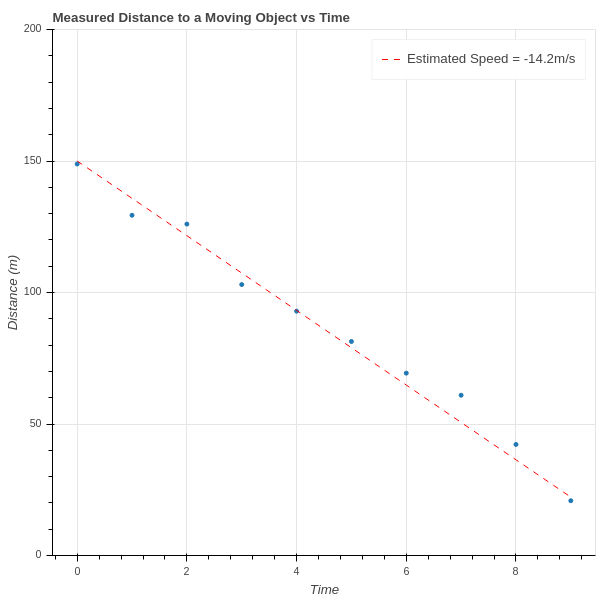
\includegraphics[width=0.5\textwidth,height=\textheight]{chapters/img/distance-vs-time.png}

}

\caption{\label{fig-dvt}Physics Experiment}

\end{figure}

On the other hand, we might look at a graph such as
Figure~\ref{fig-mpg-vs-displacement}, which plots the gas mileage of
various car models against their engine size (displacement), and observe
a general trend in which bigger engines get lower mileage. In this
situation we could ask for the best line of the form \(y=mx+b\) that
captures this relationship and use that to make general conclusions
without necessarily having an underlying theory.

\begin{figure}

{\centering 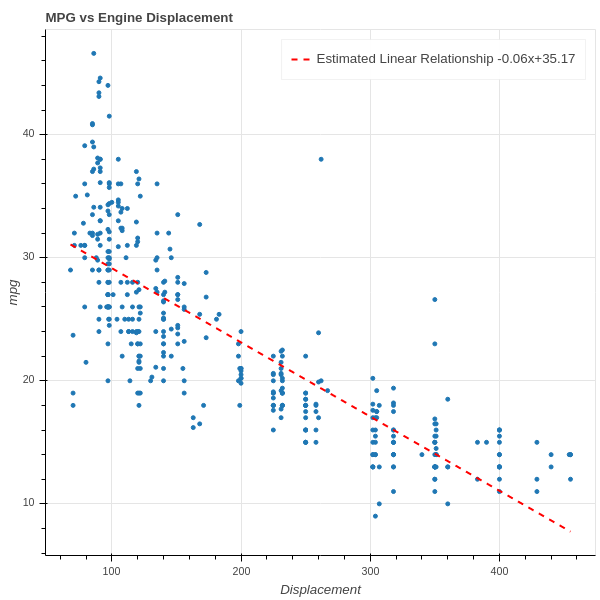
\includegraphics[width=0.5\textwidth,height=\textheight]{chapters/img/mpg-vs-displacement.png}

}

\caption{\label{fig-mpg-vs-displacement}MPG vs Displacement ( {[}1{]} )}

\end{figure}

\hypertarget{sec-Calculus}{%
\section{Least Squares (via Calculus)}\label{sec-Calculus}}

In either of the two cases above, the question we face is to determine
the line \(y=mx+b\) that ``best fits'' the data
\(\{(x_i,y_i)_{i=1}^{N}\}\). The classic approach is to determine the
equation of a line \(y=mx+b\) that minimizes the ``mean squared error'':

\[ MSE(m,b) = \frac{1}{N}\sum_{i=1}^{N} (y_i-mx_i-b)^2 \]

It's worth emphasizing that the \(MSE\) is a function of two variables
-- the slope \(m\) and the intercept \(b\) -- and that the data points
\(\{(x_i,y_i)\}\) are constants for these purposes. Furthermore, it's a
quadratic function in those two variables. Since our goal is to find
\(m\) and \(b\) that minimize the \(MSE\), we have a Calculus problem
that we can solve by taking partial derivatives and setting them to
zero.

To simplify the notation, let's abbreviate \(MSE\) by \(E\).

\[
\begin{aligned} \frac{\partial E}{\partial m} &=
\frac{1}{N}\sum_{1}^{N}-2x_i(y_i-mx_i-b) \\ \frac{\partial E}{\partial
b} &= \frac{1}{N}\sum_{1}^{N}-2(y_i-mx_i-b) \\ 
\end{aligned} 
\]

We set these two partial derivatives to zero, so we can drop the \(-2\)
and regroup the sums to obtain two equations in two unknowns (we keep
the \(\frac{1}{N}\) because it is illuminating in the final result):

\begin{equation}\protect\hypertarget{eq-LS}{}{
\begin{aligned} \frac{1}{N}(\sum_{i=1}^{N} x_i^2)m &+&
\frac{1}{N}(\sum_{i=1}^{N} x_i)b &=& \frac{1}{N}\sum_{i=1}^{N} x_i y_i
\\ \frac{1}{N}(\sum_{i=1}^{N} x_i)m &+& b &=&
\frac{1}{N}\sum_{i=1}^{N} y_{i} \\ \end{aligned}
}\label{eq-LS}\end{equation}

In these equations, notice that \(\frac{1}{N}\sum_{i=1}^{N} x_i\) is the
average (or mean) value of the \(x_i\). Let's call this
\(\overline{x}\). Similarly, \(\frac{1}{N}\sum_{i=1}^{N} y_{i}\) is the
mean of the \(y_i\), and we'll call it \(\overline{y}\). If we further
simplify the notation and write \(S_{xx}\) for
\(\frac{1}{N}\sum_{i=1}^{N} x_i^2\) and \(S_{xy}\) for
\(\frac{1}{N}\sum_{i=1}^{N}x_iy_i\) then we can write down a solution to
this system using Cramer's rule:

\begin{equation}\protect\hypertarget{eq-LSAnswer}{}{ \begin{aligned} m &=
\frac{S_{xy}-\overline{x}\overline{y}}{S_{xx}-\overline{x}^2} \\ b &=
\frac{S_{xx}\overline{y}-S_{xy}\overline{x}}{S_{xx}-\overline{x}^2} \\
\end{aligned}
}\label{eq-LSAnswer}\end{equation}

where we must have \(S_{xx}-\overline{x}^2\not=0\).

\hypertarget{sec-CalcExercises}{%
\subsection{Exercises}\label{sec-CalcExercises}}

\begin{enumerate}
\def\labelenumi{\arabic{enumi}.}
\item
  Verify that Equation~\ref{eq-LSAnswer} is in fact the solution to the
  system in Equation~\ref{eq-LS} .
\item
  Suppose that \(S_{xx}-\overline{x}^2=0\). What does that mean about
  the \(x_i\)? Does it make sense that the problem of finding the ``line
  of best fit'' fails in this case?
\end{enumerate}

\hypertarget{sec-LinAlg}{%
\section{Least Squares (via Geometry)}\label{sec-LinAlg}}

In our discussion above, we thought about our data as consisting of
\(N\) pairs \((x_i,y_i)\) corresponding to \(N\) points in the
\(xy\)-plane \(\mathbf{R}^2\). Now let's turn that picture ``on its
side'', and instead think of our data as consisting of \emph{two} points
in \(\mathbf{R}^{N}\):

\[ X=\left[\begin{matrix} x_1\cr x_2\cr \vdots\cr
x_n\end{matrix}\right] \mathrm{\ and\ } Y = \left[\begin{matrix}
y_1\cr y_2\cr \vdots\cr y_n\end{matrix}\right]
\]

Let's also introduce one other vector

\[ E = \left[\begin{matrix} 1 \cr 1 \cr \vdots \cr
1\end{matrix}\right].  
\]

First, let's assume that \(E\) and \(X\) are linearly independent. If
not, then \(X\) is a constant vector (why?) which we already know is a
problem from Section~\ref{sec-Calculus}, Exercise 2. Therefore \(E\) and
\(X\) span a plane in \(\mathbf{R}^{N}\).

\begin{figure}

{\centering 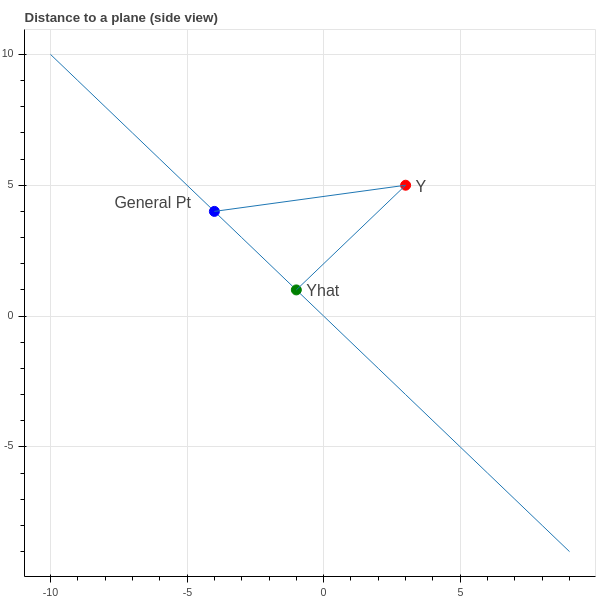
\includegraphics[width=0.5\textwidth,height=\textheight]{chapters/img/distance-to-plane.png}

}

\caption{\label{fig-perp}Distance to A Plane}

\end{figure}

Now if our data points \((x_i,y_i)\) all \emph{did} lie on a line
\(y=mx+b\), then the three vectors \(X\), \(Y\), and \(E\) would be
linearly dependent:

\[ Y = mX + bE.  \]

Since our data is only approximately linear, that's not the case. So
instead we look for an approximate solution. One way to phrase that is
to ask:

\emph{What is the point \(\hat{Y}\) in the plane \(H\) spanned by \(X\)
and \(E\) in \(\mathbf{R}^{N}\) which is closest to \(Y\)?}

If we knew this point \(\hat{Y}\), then since it lies in \(H\) we would
have \(\hat{Y}=mX+bE\) and the coefficients \(m\) and \(b\) would be a
candidate for defining a line of best fit \(y=mx+b\). Finding the point
in a plane closest to another point in \(\mathbf{R}^{N}\) is a geometry
problem that we can solve.

\textbf{Proposition:} The point \(\hat{Y}\) in the plane spanned by
\(X\) and \(E\) is the point such that the vector \(Y-\hat{Y}\) is
perpendicular to \(H\).

\textbf{Proof:} See Figure~\ref{fig-perp} for an illustration -- perhaps
you are already convinced by this, but let's be careful.
\(\hat{Y}=mX+bE\) such that \[ D = \|Y-\hat{Y}\|^2 = \|Y-mX-bE\|^2 \] is
minimal. Using some vector calculus, we have
\[ \frac{\partial D}{\partial m} =
\frac{\partial}{\partial m} (Y-mX-bE)\cdot (Y-mX-bE) =
-2(Y-mX-bE)\cdot X \] and \[ \frac{\partial D}{\partial b} =
\frac{\partial}{\partial b} (Y-mX-bE)\cdot (Y-mX-bE) =
-2(Y-mX-bE)\cdot E.  \]

So both derivatives are zero exactly when \(\hat{Y}=(Y-mX-bE)\) is
orthogonal to both \(X\) and \(E\), and therefore every vector in \(H\).

We also obtain equations for \(m\) and \(b\) just as in our first look
at this problem.

\begin{equation}\protect\hypertarget{eq-LSAnswer2}{}{ \begin{aligned} m(X\cdot E) &+ b(E\cdot E) &= (Y\cdot E) \cr
m(X\cdot X) &+ b(E\cdot X) &= (Y\cdot X) \cr \end{aligned}
}\label{eq-LSAnswer2}\end{equation}

We leave it is an exercise below to check that these are the same
equations that we obtained in Equation~\ref{eq-LSAnswer}.

\hypertarget{exercises}{%
\subsection{Exercises}\label{exercises}}

\begin{enumerate}
\def\labelenumi{\arabic{enumi}.}
\tightlist
\item
  Verify that Equation~\ref{eq-LSAnswer} and Equation~\ref{eq-LSAnswer2}
  are equivalent.
\end{enumerate}

\hypertarget{sec-Multivariate-calculus}{%
\section{The Multivariate Case
(Calculus)}\label{sec-Multivariate-calculus}}

Having worked through the problem of finding a ``line of best fit'' from
two points of view, let's look at a more general problem. We looked
above at a scatterplot showing the relationship between gas mileage and
engine size (displacement). There are other factors that might
contribute to gas mileage that we want to consider as well -- for
example:

\begin{itemize}
\tightlist
\item
  a car that is heavy compared to its engine size may get worse mileage
\item
  a sports car with a drive train that gives fast acceleration as
  compared to a car with a transmission designed for long trips may have
  different mileage for the same engine size.
\end{itemize}

Suppose we wish to use engine displacement, vehicle weight, and
acceleration all together to predict mileage. Instead of looking points
\((x_i,y_i)\) where \(x_i\) is the displacement of the \(i^{th}\) car
model and we try to predict a value \(y\) from a corresponding \(x\) as
\(y=mx+b\) -- let's look at a situation in which our measured value
\(y\) depends on multiple variables -- say displacement \(d\), weight
\(w\), and acceleration \(a\) with \(k=3\) -- and we are trying to find
the best linear equation

\begin{equation}\protect\hypertarget{eq-multivariate}{}{ 
y=m_1 d + m_2 w + m_3 a +b 
}\label{eq-multivariate}\end{equation}

But to handle this situation more generally we need to adopt a
convention that will allow us to use indexed variables instead of \(d\),
\(w\), and \(a\). We will use the \emph{tidy} data convention.

\textbf{Tidy Data:} A dataset is tidy if it consists of values
\(x_{ij}\) for \(i=1,\ldots,N\) and \(j=1,\ldots, k\) so that:

\begin{itemize}
\tightlist
\item
  the row index corresponds to a \emph{sample} -- a set of measurements
  from a single event or item;
\item
  the column index corresponds to a \emph{feature} -- a particular
  property measured for all of the events or items.
\end{itemize}

In our case,

\begin{itemize}
\tightlist
\item
  the \emph{samples} are the different types of car models,
\item
  the \emph{features} are the properties of those car models.
\end{itemize}

For us, \(N\) is the number of different types of cars, and \(k\) is the
number of properties we are considering. Since we are looking at
displacement, weight, and acceleration, we have \(k=3\).

So the ``independent variables'' for a set of data that consists of
\(N\) samples, and \(k\) measurements for each sample, can be
represented by a \(N\times k\) matrix

\[ X = \left(\begin{matrix} x_{11} & x_{12} & \cdots & x_{1k} \\
x_{21} & x_{22} & \cdots & x_{2k} \\ \vdots & \vdots & \ddots & \vdots
\\ x_{N1} & x_{k2} & \cdots & x_{Nk} \\ \end{matrix}\right)
\]

and the measured dependent variables \(Y\) are a column vector \[ Y =
\left[\begin{matrix} y_1 \\ y_2 \\ \vdots \\ y_N\end{matrix}\right].
\]

If \(m_1,\ldots, m_k\) are ``slopes'' associated with these properties
in Equation~\ref{eq-multivariate}, and \(b\) is the ``intercept'', then
the predicted value \(\hat{Y}\) is given by a matrix equation

\[ 
\hat{Y} = X\left[\begin{matrix} m_1 \\ m_2 \\ \cdots \\
m_k\end{matrix}\right]+\left[\begin{matrix} 1 \\ 1 \\ \cdots \\
1\end{matrix}\right]b 
\]

and our goal is to choose these parameters \(m_i\) and \(b\) to make the
mean squared error:

\[ MSE(m_1,\ldots, m_k,b) = \|Y-\hat{Y}\|^2 = \sum_{i=1}^{N} (y_i -
\sum_{j=1}^{k} x_{ij}m_j -b )^2.
\]

Here we are summing over the \(N\) different car models, and for each
model taking the squared difference between the true mileage \(y_i\) and
the ``predicted'' mileage \(\sum_{j=1}^{k} x_{ij}m_j +b\). We wish to
minimize this MSE.

Let's make one more simplification. The intercept variable \(b\) is
annoying because it requires separate treatment from the \(m_i\). But we
can use a trick to eliminate the need for special treatment. Let's add a
new feature to our data matrix (a new column) that has the constant
value \(1\).

\[ X = \left(\begin{matrix} x_{11} & x_{12} & \cdots & x_{1k} & 1\\
x_{21} & x_{22} & \cdots & x_{2k} & 1\\ \vdots & \vdots & \ddots &
\vdots & 1\\ x_{N1} & x_{k2} & \cdots & x_{Nk} & 1\\
\end{matrix}\right)
\]

Now our data matrix \(X\) is \(N\times(k+1)\) and we can put our
``intercept'' \(b=m_{k+1}\) into our vector of ``slopes''
\(m_1, \ldots, m_k,m_{k+1}\):

\[ \hat{Y} = X\left[\begin{matrix} m_1 \\ m_2 \\ \cdots \\ m_k \\
m_{k+1}\end{matrix}\right]
\]

and our MSE becomes

\[ 
MSE(M) = \|Y - XM\|^2
\]

where

\[ M=\left[\begin{matrix} m_1 \\ m_2 \\ \cdots \\ m_k \\
m_{k+1}\end{matrix}\right].
\]

\textbf{Remark:} Later on (see \{Section~\ref{sec-centered}\}) we will
see that if we ``center'' our features about their mean, by subtracting
the average value of each column of \(X\) from that column; and we also
subtract the average value of \(Y\) from the entries of \(Y\), then the
\(b\) that emerges from the least squares fit is zero. As a result,
instead of adding a column of \(1\)'s, you can change coordinates to
center each feature about its mean, and keep your \(X\) matrix
\(N\times k\).

The Calculus approach to minimizing the \(MSE\) is to take its partial
derivatives with respect to the \(m_{i}\) and set them to zero. Let's
first work out the derivatives in a nice form for later.

\textbf{Proposition:} The gradient of \(MSE(M)=E\) is given by

\begin{equation}\protect\hypertarget{eq-gradient}{}{ 
\nabla E = \left[\begin{matrix} \df{M_1}E \\ \df{M_2}E \\ \vdots \\
\df{m_{M+1}}E\end{matrix}\right] = -2 X^{\intercal}Y + 2
X^{\intercal}XM 
}\label{eq-gradient}\end{equation}

where \(X^{\intercal}\) is the transpose of \(X\).

\textbf{Proof:} First, remember that the \(ij\) entry of
\(X^{\intercal}\) is the \(ji\) entry of \(X\). Also, we will use the
notation \(X[j,:]\) to mean the \(j^{th}\) row of \(X\) and \(X[:,i]\)
to mean the \(i^{th}\) column of \(X\). (This is copied from the Python
programming language; the `:' means that index runs over all
possibilities).

Since \[ E = \sum_{j=1}^{N} (Y_j-\sum_{s=1}^{k+1} X_{js}M_{s})^2 \] we
compute:
\begin{equation}\protect\hypertarget{eq-gradient2}{}{\begin{aligned} \df{M_t}E &= -2\sum_{j=1}^{N}
X_{jt}(Y_{j}-\sum_{s=1}^{k+1} X_{js}M_{s}) \\ &= -2(\sum_{j=1}^{N}
Y_{j}X_{jt} - \sum_{j=1}^{N}\sum_{s=1}^{k+1} X_{jt}X_{js}M_{s}) \\ &=
-2(\sum_{j=1}^{N} X^{\intercal}_{tj}Y_{j}
-\sum_{j=1}^{N}\sum_{s=1}^{k+1} X^{\intercal}_{tj}X_{js}M_{s}) \\ &=
-2(X^{\intercal}[t,:]Y - \sum_{s=1}^{k+1}\sum_{j=1}^{N}
X^{\intercal}_{tj}X_{js}M_{s}) \\ &= -2(X^{\intercal}[t,:]Y -
\sum_{s=1}^{k+1} (X^{\intercal}X)_{ts}M_{s}) \\ &=
-2[X^{\intercal}[t,:]Y - (X^{\intercal}X](t,:)M)\\
\end{aligned}}\label{eq-gradient2}\end{equation}

Stacking up the different rows to make \(E\) yields the desired formula.

\textbf{Proposition:} Assume that \(D=X^{\intercal}X\) is invertible
(notice that it is a \((k+1)\times(k+1)\) square matrix so this makes
sense). The solution \(M\) to the multivariate least squares problem is
\begin{equation}\protect\hypertarget{eq-Msolution}{}{ M =
D^{-1}X^{\intercal}Y }\label{eq-Msolution}\end{equation} and the
``predicted value'' \(\hat{Y}\) for \(Y\) is
\begin{equation}\protect\hypertarget{eq-projection}{}{ 
\hat{Y} = XD^{-1}X^{\intercal}Y.
}\label{eq-projection}\end{equation}

\hypertarget{the-multivariate-case-geometry}{%
\section{The Multivariate Case
(Geometry)}\label{the-multivariate-case-geometry}}

Let's look more closely at the equation obtained by setting the gradient
of the error, Equation~\ref{eq-gradient}, to zero. Remember that \(M\)
is the unknown vector in this equation, everything else is known:

\[ X^{\intercal}Y = X^{\intercal}XM \]

Here is how to think about this:

\begin{enumerate}
\def\labelenumi{\arabic{enumi}.}
\item
  As \(M\) varies, the \(N\times 1\) matrix \(XM\) varies over the space
  spanned by the columns of the matrix \(X\). So as \(M\) varies \(XM\)
  is a general element of the subspace \(H\) of \(R^{N}\) spanned by the
  \(k+1\) columns of \(X\).
\item
  The product \(X^{\intercal}XM\) is a \((k+1)\times 1\) matrix. Each
  entry is the dot product of the general element of \(H\) with one of
  the \(k+1\) basis vectors of \(H\).
\item
  The product \(X^{\intercal}Y\) is a \((k+1)\times 1\) matrix whose
  entries are the dot product of the basis vectors of \(H\) with \(Y\).
\end{enumerate}

Therefore, this equation asks for us to find \(M\) so that the vector
\(XM\) in \(H\) has the same dot products with the basis vectors of
\(H\) as \(Y\) does. The condition

\[ X^{\intercal}\cdot (Y-XM)=0 \]

says that \(Y-XM\) is orthogonal to \(H\). This argument establishes the
following proposition.

\textbf{Proposition:} Just as in the simple one-dimensional case, the
predicted value \(\hat{Y}\) of the least squares problem is the point in
\(H\) closest to \(Y\) -- or in other words the point \(\hat{Y}\) in
\(H\) such that \(Y-\hat{Y}\) is perpendicular to \(H\).

\hypertarget{orthogonal-projection}{%
\subsection{Orthogonal Projection}\label{orthogonal-projection}}

Recall that we introduced the notation \(D=X^{\intercal}X\), and let's
assume, for now, that \(D\) is an invertible matrix. We have the formula
(see Equation~\ref{eq-projection}):
\[ \hat{Y} = XD^{-1}X^{\intercal}Y.  \] \textbf{Proposition:} The matrix
\(P=XD^{-1}X^{\intercal}\) is an \(N\times N\) matrix called the
orthogonal projection operator onto the subspace \(H\) spanned by the
columns of \(X\). It has the following properties:

\begin{itemize}
\tightlist
\item
  \(PY\) belongs to the subspace \(H\) for any \(Y\in\mathbf{R}^{N}\).
\item
  \((Y-PY)\) is orthogonal to \(H\).
\item
  \(P*P = P\).
\end{itemize}

\textbf{Proof:} First of all, \(PY=XD^{-1}X^{\intercal}Y\) so \(PY\) is
a linear combination of the columns of \(X\) and is therefore an element
of \(H\). Next, we can compute the dot product of \(PY\) against a basis
of \(H\) by computing

\[ X^{\intercal}PY = X^{\intercal}XD^{-1}X^{\intercal}Y =
X^{\intercal}Y 
\]

since \(X^{\intercal}X=D\). This equation means that
\(X^{\intercal}(Y-PY)=0\) which tells us that \(Y-PY\) has dot product
zero with a basis for \(H\). Finally,

\[ PP = XD^{-1}X^{\intercal}XD^{-1}X^{\intercal} =
XD^{-1}X^{\intercal}=P.  
\]

It should be clear from the above discussion that the matrix
\(D=X^{\intercal}X\) plays an important role in the study of this
problem. In particular it must be invertible or our analysis above
breaks down. In the next section we will look more closely at this
matrix and what information it encodes about our data.

\hypertarget{sec-centered}{%
\section{Centered coordinates}\label{sec-centered}}

Recall from last section that the matrix \(D=X^{\intercal}X\) is of
central importance to the study of the multivariate least squares
problem. Let's look at it more closely.

\textbf{Lemma:} The \(i,j\) entry of \(D\) is the dot product \[
D_{ij}=X[:,i]\cdot X[:,j] \] of the \(i^{th}\) and \(j^{th}\) columns of
\(X\).

\textbf{Proof:} In the matrix multiplication \(X^{\intercal}X\), the
\(i^{th}\) row of \(X^{\intercal}\) gets ``dotted'' with the \(j^{th}\)
column of \(X\) to product the \(i,j\) entry. But the \(i^{th}\) row of
\(X^{\intercal}\) is the \(i^{th}\) column of \(X\), as asserted in the
statement of the lemma.

A crucial point in our construction above relied on the matrix \(D\)
being invertible. The following Lemma shows that \(D\) fails to be
invertible only when the different features (the columns of \(X\)) are
linearly dependent.

\textbf{Lemma:} \(D\) is not invertible if and only if the columns of
\(X\) are linearly dependent.

\textbf{Proof:} If the columns of \(X\) are linearly dependent, then
there is a nonzero vector \(m\) so that \(Xm=0\). In that case clearly
\(Dm=X^{\intercal}Xm=0\) so \(D\) is not invertible. Suppose \(D\) is
not invertible. Then there is a nonzero vector \(m\) with
\(Dm=X^{\intercal}Xm=0\). This means that the vector \(Xm\) is
orthogonal to all of the columns of \(X\). Since \(Xm\) belongs to the
span \(H\) of the columns of \(X\), if it is orthogonal to \(H\) it must
be zero.

In fact, the matrix \(D\) captures some important statistical measures
of our data, but to see this clearly we need to make a slight change of
basis. First recall that \(X[:,k+1]\) is our column of all \(1\), added
to handle the intercept. As a result, the dot product
\(X[:,i]\cdot X[:,k+1]\) is the sum of the entries in the \(i^{th}\)
column, and so if we let \(\mu_{i}\) denote the average value of the
entries in column \(i\), we have \[ \mu_{i} = \frac{1}{N}(X[:,i]\cdot
X[:,k+1]) \]

Now change the matrix \(X\) by elementary column operations to obtain a
new data matrix \(X_{0}\) by setting \[ X_{0}[:,i] =
X[:,i]-\frac{1}{N}(X[:,i]\cdot X[:,k+1])X[:,k+1] =
X[:,i]-\mu_{i}X[:,k+1] \] for \(i=1,\ldots, k\).

In terms of the original data, we are changing the measurement scale of
the data so that each feature has average value zero, and the subspace
\(H\) spanned by the columns of \(X_{0}\) is the same as that spanned by
the columns of \(X\). Using \(X_{0}\) instead of \(X\) for our least
squares problem, we get

\[ \hat{Y} = X_{0}D_{0}^{-1}X_{0}^{\intercal}Y \]

and

\[ M_{0} = D_{0}^{-1}X_{0}^{\intercal}Y \]

where \(D_{0}=X_{0}^{\intercal}X_{0}.\)

\textbf{Proposition:} The matrix \(D_{0}\) has a block form. Its upper
left block is a \(k\times k\) symmetric block with entries
\[ (D_{0})_{ij} =
(X[:,i]-\mu_{i}X[:,k+1])\cdot(X[:,j]-\mu_{j}X[:,k+1]) \] Its
\((k+1)^{st}\) row and column are all zero, except for the
\((k+1),(k+1)\) entry, which is \(N\).

\textbf{Proof:} This follows from the fact that the last row and column
entries are (for \(i\not=k+1\)): \[ (X[:,i]-\mu_{i}X[:,k+1])\cdot
X[:,k+1] = (X[:,i]\cdot X[:,k+1])-N\mu_{i} = 0 \] and for \(i=k+1\) we
have \(X[:,k+1]\cdot X[:,k+1]=N\) since that column is just \(N\)
\(1\)'s.

\textbf{Proposition:} If the \(x\) coordinates (the features) are
centered so that they have mean zero, then the intercept \(b\) is
\[ \overline{Y} =
\frac{1}{N}\sum y_{i}.  \]

\textbf{Proof:} By centering the coordinates, we replace the matrix
\(X\) by \(X_{0}\) and \(D\) by \(D_{0}\). and we are trying to minimize
\(\|Y-X_{0}M_{0}\|^2\). Use the formula from Equation~\ref{eq-Msolution}
to see that \[ M_{0} = D_{0}^{-1}X_{0}^{\intercal}Y.  \] The \(b\) value
we are interested in is the last entry \(m_{k+1}\) in \(M_{0}\). From
the block form of \(D_{0}\), we know that \(D_{0}^{-1}\) has bottom row
and last column zero except for \(1/N\) in position
\((k+1)\times(k+1)\). Also \(X_{0}^{\intercal}\) has last row consisting
entirely of \(1\). So the bottom entry of \(X_{0}^{\intercal}Y\) is
\(\sum_{i=1}^{N} y_{i}\), and the bottom entry \(b\) of
\(D_{0}^{-1}X_{0}^{\intercal}Y\) is \[ \mu_{Y} =
\frac{1}{N}\sum_{i=1}^{N} y_{i}.  \] as claimed.

\textbf{Corollary:} If we make a further change of coordinates to define
\[
Y_{0} = Y - \mu_{Y}\left[\begin{matrix} 1 \\ 1 \\ \vdots \\
1\end{matrix}\right] \] then the associated \(b\) is zero. As a result
we can forget about the extra column of \(1's\) that we added to \(X\)
to account for it and reduce the dimension of our entire problem by
\(1\).

Just to recap, if we center our data so that \(\mu_{Y}=0\) and
\(\mu_{i}=0\) for \(i=1,\ldots, k\), then the least squares problem
reduces to minimizing \[ E(M) = \|Y-XM\|^2 \] where \(X\) is the
\(N\times k\) matrix with \(j^{th}\) row
\((x_{j1},x_{j2},\ldots, x_{jk})\) for \(j=1,\ldots, N\) and the
solutions are as given in Equation~\ref{eq-Msolution} and
Equation~\ref{eq-projection}.

\hypertarget{caveats-about-linear-regression}{%
\section{Caveats about Linear
Regression}\label{caveats-about-linear-regression}}

\hypertarget{basic-considerations}{%
\subsection{Basic considerations}\label{basic-considerations}}

Reflecting on our long discussion up to this point, we should take note
of some of the potential pitfalls that lurk in the use of linear
regression.

\begin{enumerate}
\def\labelenumi{\arabic{enumi}.}
\item
  When we apply linear regression, we are explicitly assuming that the
  variable \(Y\) is associated to \(X\) via linear equations. This is a
  big assumption!
\item
  When we use multilinear regression, we are assuming that changes in
  the different features have independent effects on the target variable
  \(y\). In other words, suppose that \(y=ax_1+bx_2\). Then an increase
  of \(x_1\) by \(1\) increases \(y\) by \(a\), and an increase of
  \(x_2\) by \(1\) increases \(y\) by \(b\). These effects are
  independent of one another and combine to yield an increase of
  \(a+b\).
\item
  We showed in our discussion above that linear regression problem has a
  solution when the matrix \(D=X^{\intercal}X\) is invertible, and this
  happens when the columns of \(D\) are linearly independent. When
  working with real data, which is messy, we could have a situation in
  which the features we are studying are, in fact, dependent -- but
  because of measurement error, the samples that we collected aren't. In
  this case, the matrix \(D\) will be ``close'' to being non-invertible,
  although formally still invertible. In this case, computing \(D^{-1}\)
  leads to numerical instability and the solution we obtain is very
  unreliable.
\end{enumerate}

\hypertarget{simpsons-effect}{%
\subsection{Simpson's Effect}\label{simpsons-effect}}

Simpson's effect is a famous phenomenon that illustrates that linear
regression can be very misleading in some circumstances. It is often a
product of ``pooling'' results from multiple experiments. Suppose, for
example, that we are studying the relationship between a certain measure
of blood chemistry and an individual's weight gain or less on a
particular diet. We do our experiments in three labs, the blue, green,
and red labs. Each lab obtains similar results -- higher levels of the
blood marker correspond to greater weight gain, with a regression line
of slope around 1. However, because of differences in the population
that each lab is studying, some populations are more susceptible to
weight gain and so the red lab sees a mean increase of almost 9 lbs
while the blue lab sees a weight gain of only 3 lbs on average.

The three groups of scientists pool their results to get a larger sample
size and do a new regression. Surprise! Now the regression line has
slope \(-1.6\) and increasing amounts of the marker seem to lead to
\emph{less} weight gain!

This is called Simpson's effect, or Simpson's paradox, and it shows that
unknown factors (confounding factors) may cause linear regression to
yield misleading results. This is particularly true when data from
experiments conducted under different conditions is combined; in this
case, the differences in experimental setting, called \emph{batch
effects}, can throw off the analysis very dramatically. See
Figure~\ref{fig-simpsons} .

\begin{figure}

{\centering 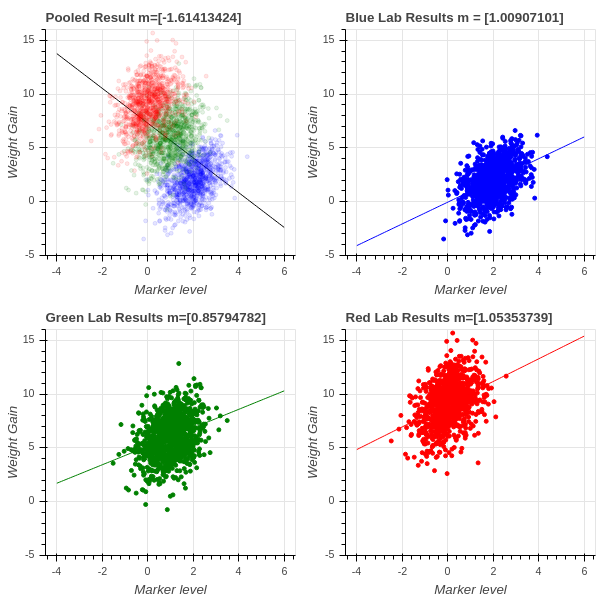
\includegraphics[width=0.5\textwidth,height=\textheight]{chapters/img/SimpsonsEffect.png}

}

\caption{\label{fig-simpsons}Simpson's Effect}

\end{figure}

\hypertarget{exercises-1}{%
\subsection{Exercises}\label{exercises-1}}

\begin{enumerate}
\def\labelenumi{\arabic{enumi}.}
\tightlist
\item
  When proving that \(D\) is invertible if and only if the columns of
  \(X\) are linearly independent, we argued that if
  \(X^{\intercal}Xm=0\) for a nonzero vector \(m\), then \(Xm\) is
  orthogonal to the span of the columns of \(X\), and is also an element
  of that span, and is therefore zero. Provide the details: show that if
  \(H\) is a subspace of \(\mathbf{R}^{N}\), and \(x\) is a vector in
  \(H\) such that \(x\cdot h=0\) for all \(h\in H\), then \(x=0\).
\end{enumerate}

\bookmarksetup{startatroot}

\hypertarget{principal-component-analysis}{%
\chapter{Principal Component
Analysis}\label{principal-component-analysis}}

\hypertarget{introduction}{%
\section{Introduction}\label{introduction}}

Suppose that, as usual, we begin with a collection of measurements of
different features for a group of samples. Some of these measurements
will tell us quite a bit about the dif mergefference among our samples,
while others may contain relatively little information. For example, if
we are analyzing the effect of a certain weight loss regimen on a group
of people, the age and weight of the subjects may have a great deal of
influence on how successful the regimen is, while their blood pressure
might not. One way to help identify which features are more significant
is to ask whether or not the feature varies a lot among the different
samples. If nearly all the measurements of a feature are the same, it
can't have much power in distinguishing the samples, while if the
measurements vary a great deal then that feature has a chance to contain
useful information.

In this section we will discuss a way to measure the variability of
measurements and then introduce principal component analysis (PCA). PCA
is a method for finding which linear combinations of measurements have
the greatest variability and therefore might contain the most
information. It also allows us to identify combinations of measurements
that don't vary much at all. Combining this information, we can
sometimes replace our original system of features with a smaller set
that still captures most of the interesting information in our data, and
thereby find hidden characteristics of the data and simplify our
analysis a great deal.

\hypertarget{variance-and-covariance}{%
\section{Variance and Covariance}\label{variance-and-covariance}}

\hypertarget{variance}{%
\subsection{Variance}\label{variance}}

Suppose that we have a collection of measurements \((x_1,\ldots, x_N)\)
of a particular feature \(X\). For example, \(x_i\) might be the initial
weight of the \(ith\) participant in our weight loss study. The mean of
the values \((x_1,\ldots, x_N)\) is

\[
\mu_{X} = \frac{1}{N}\sum_{i=1}^{N} x_{i}.
\]

The simplest measure of the variability of the data is called its
\emph{variance.}

\textbf{Definition:} The (sample) variance of the data
\(x_1,\ldots, x_N\) is

\begin{equation}\protect\hypertarget{eq-variance}{}{
\sigma_{X}^2 = \frac{1}{N}\sum_{i=1}^{N} \left(x_{i}-\mu_{X}\right)^2 = \frac{1}{N}\left(\sum_{i=1}^{N} x_{i}^2\right)- \mu_{X}^2
}\label{eq-variance}\end{equation}

The square root of the variance is called the \emph{standard deviation.}

As we see from the formula, the variance is a measure of how `spread
out' the data is from the mean.

Recall that in our discussion of linear regression we thought of our set
of measurements \(x_1,\ldots, x_N\) as a vector -- it's one of the
columns of our data matrix. From that point of view, the variance has a
geometric interpretation -- it is \(\frac{1}{N}\) times the square of
the distance from the point \(X=(x_1,\ldots, x_N)\) to the point
\(\mu_{X}(1,1,\ldots,1)=\mu_{X}E\):

\begin{equation}\protect\hypertarget{eq-variancedot}{}{
\sigma_{X}^2 = \frac{1}{N}(X-\mu_{X}E)\cdot(X-\mu_{X}E)  = \frac{1}{N}\|X-\mu_{X}E\|^2.
}\label{eq-variancedot}\end{equation}

\hypertarget{covariance}{%
\subsection{Covariance}\label{covariance}}

The variance measures the dispersion of measures of a single feature.
Often, we have measurements of multiple features and we might want to
know something about how two features are related. The \emph{covariance}
is a measure of whether two features tend to be related, in the sense
that when one increases, the other one increases; or when one increases,
the other one decreases.

\textbf{Definition:} Given measurements \((x_1,\ldots, x_N)\) and
\((y_1,\ldots, y_N)\) of two features \(X\) and \(Y\), the covariance of
\(X\) and \(Y\) is

\begin{equation}\protect\hypertarget{eq-covariancedot}{}{
\sigma_{XY} = \frac{1}{N}\sum_{i=1}^{N} (x_i-\mu_{X})(y_i-\mu_{Y})
}\label{eq-covariancedot}\end{equation}

There is a nice geometric interpretation of this, as well, in terms of
the dot product. If \(X=(x_1,\ldots, x_N)\) and \(Y=(y_1\ldots,y_N)\)
then

\[
\sigma_{XY} = \frac{1}{N} ((X-\mu_{X}E)\cdot (Y-\mu_{Y}E)).
\]

From this point of view, we can see that \(\sigma_{XY}\) is positive if
the \(X-\mu_{X}E\) and \(Y-\mu_{Y}E\) vectors ``point roughly in the
same direction'' and its negative if they ``point roughly in the
opposite direction.''

\hypertarget{correlation}{%
\subsection{Correlation}\label{correlation}}

One problem with interpreting the variance and covariance is that we
don't have a scale -- for example, if \(\sigma_{XY}\) is large and
positive, then we'd like to say that \(X\) and \(Y\) are closely
related, but it could be just that the entries of \(X-\mu_{X}E\) and
\(Y-\mu_{Y}E\) are large. Here, though, we can really take advantage of
the geometric interpretation. Recall that the dot product of two vectors
satisfies the formula

\[
a \cdot b = \|a\|\|b\|\cos(\theta)
\]

where \(\theta\) is the angle between \(a\) and \(b\). So

\[
\cos(\theta) = \frac{a\cdot b}{\|a\|\|b\|}.
\]

Let's apply this to the variance and covariance, by noticing that

\[
\frac{(X-\mu_{X}E)\cdot (Y-\mu_{Y}E)}{\|(X-\mu_{X}E)\|\|(Y-\mu_{Y}E)\|} = \frac{\sigma_{XY}}{\sigma_{XX}\sigma_{YY}}
\]

so the quantity

\begin{equation}\protect\hypertarget{eq-rxy}{}{
r_{XY} = \frac{\sigma_{XY}}{\sigma_{X}\sigma_{Y}}
}\label{eq-rxy}\end{equation}

measures the cosine of the angle between the vectors \(X-\mu_{X}E\) and
\(Y-\mu_{Y}E\).

\textbf{Definition:} The quantity \(r_{XY}\) defined in
Equation~\ref{eq-rxy} is called the (sample) \emph{correlation
coefficient} between \(X\) and \(Y\). We have \(0\le |r_{XY}|\le 1\)
with \(r_{XY}=\pm 1\) if and only if the two vectors \(X-\mu_{X}\) and
\(Y-\mu_{Y}\) are collinear in \(\mathbf{R}^{N}\).

*Figure~\ref{fig-corrfig} illustrates data with different values of the
correlation coefficient.

\begin{figure}

{\centering 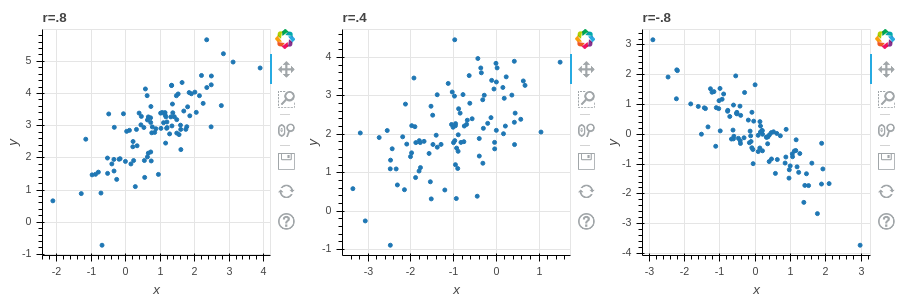
\includegraphics[width=0.5\textwidth,height=\textheight]{chapters/img/correlation.png}

}

\caption{\label{fig-corrfig}Correlation}

\end{figure}

\hypertarget{sec-covarmat}{%
\subsection{The covariance matrix}\label{sec-covarmat}}

In a typical situation we have many features for each of our (many)
samples, that we organize into a data matrix \(X\). To recall, each
column of \(X\) corresponds to a feature that we measure, and each row
corresponds to a sample. For example, each row of our matrix might
correspond to a person enrolled in a study, and the columns correspond
to height (cm), weight (kg), systolic blood pressure, and age (in
years):

\begin{longtable}[]{@{}lrrrr@{}}
\caption{A sample data matrix \(X\)}\tabularnewline
\toprule()
sample & Ht & Wgt & Bp & Age \\
\midrule()
\endfirsthead
\toprule()
sample & Ht & Wgt & Bp & Age \\
\midrule()
\endhead
A & 180 & 75 & 110 & 35 \\
B & 193 & 80 & 130 & 40 \\
\ldots{} & \ldots{} & \ldots{} & \ldots{} & \ldots{} \\
U & 150 & 92 & 105 & 55 \\
\bottomrule()
\end{longtable}

If we have multiple features, as in this example, we might be interested
in the variance of each feature and all of their mutual covariances.
This ``package'' of information can be obtained ``all at once'' by
taking advantage of some matrix algebra.

\textbf{Definition:} Let \(X\) be a \(N\times k\) data matrix, where the
\(k\) columns of \(X\) correspond to different features and the \(N\)
rows to different samples. Let \(X_{0}\) be the centered version of this
data matrix, obtained by subtracting the mean \(\mu_{i}\) of column
\(i\) from all the entries \(x_{si}\) in that column. Then the
\(k\times k\) symmetric matrix

\[
D_{0} = \frac{1}{N}X_{0}^{\intercal}X_{0}
\]

is called the (sample) covariance matrix for the data.

\textbf{Proposition:} The diagonal entries \(d_{ii}\) of \(D_{0}\) are
the variances of the columns of \(X\):

\[
d_{ii} = \sigma_{i}^2 = \frac{1}{N}\sum_{s=1}^{N}(x_{si}-\mu_i)^2
\]

and the off-diagonal entries \(d_{ij} = d_{ji}\) are the covariances of
the \(i^{th}\) and \(j^{th}\) columns of \(X\):

\[
d_{ij} = \sigma_{ij} = \frac{1}{N}\sum_{s=1}^{N}(x_{si}-\mu_{i})(x_{sj}-\mu_{j})
\]

The sum of the diagonal entries, the trace of \(D_{0}\) is the
\textbf{total} variance of the data.

\textbf{Proof:} This follows from the definitions, but it's worth
checking the details, which we leave as an exercise.

\hypertarget{sec-visualizecovar}{%
\subsection{Visualizing the covariance
matrix}\label{sec-visualizecovar}}

If the number of features in the data is not too large, a density matrix
plot provides a tool for visualizing the covariance matrix of the data.
A density matrix plot is an \(k\times k\) grid of plots (where \(k\) is
the number of features). The entry with \((i,j)\) coordinates in the
grid is a scatter plot of the \(i^{th}\) feature against the \(j^{th}\)
one if \(i\not=j\), and is a histogram of the \(i^{th}\) variable if
\(i=j\).

*Figure~\ref{fig-density0} is an example of a density matrix plot for a
dataset with \(50\) samples and \(2\) features. This data has been
centered, so it can be represented in a \(50\times 2\) data matrix
\(X_{0}\). The upper left and lower right graphs are scatter plots of
the two columns, while the lower left and upper right are the histograms
of the columns.

\begin{figure}

{\centering 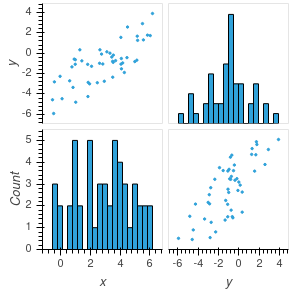
\includegraphics[width=0.5\textwidth,height=\textheight]{chapters/img/density2x2.png}

}

\caption{\label{fig-density0}Density Matrix Plot}

\end{figure}

\hypertarget{linear-combinations-of-features-scores}{%
\subsection{Linear Combinations of Features
(Scores)}\label{linear-combinations-of-features-scores}}

Sometimes useful information about our data can be revealed if we
combine different measurements together to obtain a ``hybrid'' measure
that captures something interesting. For example, in the Auto MPG
dataset that we studied in the section on Linear Regression, we looked
at the influence of both vehicle weight \(w\) and engine displacement
\(e\) on gas mileage; perhaps their is some value in considering a
hybrid ``score'' defined as \[
S = aw + be
\] for some constants \(a\) and \(b\) -- maybe by choosing a good
combination we could find a better predictor of gas mileage than using
one or the other of the features individually.

As another example, suppose we are interested in the impact of the
nutritional content of food on weight gain in a study. We know that both
calorie content and the level dietary fiber contribute to the weight
gain of participants eating this particular food; maybe there is some
kind of combined ``calorie/fiber'' score we could introduce that
captures the impact of that food better.

Finally, when we assign grades in a course, we typically compute a
weighted combination of the scores of each student on a series of
assignments. Such a combination is another example of a ``score'' and
may help explain the origin of the term.

\textbf{Definition:} Let \(X_{0}\) be a (centered) \(N\times k\) data
matrix giving information about \(k\) features for each of \(N\)
samples. A linear synthetic feature, or a linear score, is a linear
combination of the \(k\) features. The linear score is defined by
constants \(a_{1},\ldots, a_{k}\) so that If \(y_{1},\ldots, y_{k}\) are
the values of the features for a particular sample, then the linear
score for that sample is

\[
S = a_{1}y_{1}+a_{2}y_{2}+\cdots+a_{k}y_{k}
\]

\textbf{Lemma:} The values of the linear score for each of the \(N\)
samples can be calculated as

\begin{equation}\protect\hypertarget{eq-linearscore}{}{
\left[\begin{matrix} S_{1} \\ \vdots \\ S_{N}\\ \end{matrix}\right] =
X_{0}\left[
\begin{matrix} a_{1} \\ \vdots \\ a_{k}\end{matrix}\right].
}\label{eq-linearscore}\end{equation}

\textbf{Proof:} Multiplying a matrix by a column vector computes a
linear combination of the columns -- that's what this lemma says.
Exercise 3 asks you to write out the indices and make sure you believe
this.

\hypertarget{mean-and-variance-of-scores}{%
\subsection{Mean and variance of
scores}\label{mean-and-variance-of-scores}}

When we combine features to make a hybrid score, we assume that the
features were centered to begin with, so that each features has mean
zero. As a result, the mean of the hybrid features is again zero.

\textbf{Lemma:} A linear combination of features with mean zero again
has mean zero.

\textbf{Proof:} Let \(S_{i}\) be the score for the \(i^{th}\) sample, so
\[
S_{i} = \sum_{j=1}^{k} x_{ij}a_{j}.
\] where \(X_{0}\) has entries \(x_{ij}\). Then the mean value of the
score is \[
\mu_{S} = \frac{1}{k}\sum_{i=1}^{N} S_{i} = \frac{1}{N}\sum_{i=1}^{N}\sum_{j=1}^{k} x_{ij}a_{j}.
\] Reversing the order of the sum yields \[
\mu_{S} = \frac{1}{N}\sum_{j=1}^{k}\sum_{i=1}^{N} x_{ij}a_{j} = \sum_{j=1}^{k} a_{j}\frac{1}{N}(\sum_{i=1}^{N} x_{ij})=
\sum_{j=1}^{k}a_{j}\mu_{j}=0
\] where \(\mu_{j}=0\) is the mean of the \(j^{th}\) feature (column) of
\(X_{0}\).

The variance is more interesting, and gives us an opportunity to put the
covariance matrix to work. Remember from Equation~\ref{eq-variancedot}
that, since a score \(S\) has mean zero, it's variance is
\(\sigma_{S}^2=\frac{1}{N}S\cdot S\) -- where here the score \(S\) is
represented by the column vector with entries \(S_{1},\ldots S_{k}\) as
in Equation~\ref{eq-linearscore}.

\textbf{Lemma:} The variance of the score \(S\) with weights
\(a_1,\ldots a_k\) is \begin{equation}\protect\hypertarget{eq-ada}{}{
\sigma_{S}^2 = a^{\intercal}D_{0}a = \left[\begin{matrix}a_{1} & \cdots & a_{k}\end{matrix}\right]D_{0}
\left[\begin{matrix} a_{1} \\ \vdots \\ a_{k}\end{matrix}\right]
}\label{eq-ada}\end{equation} More generally, if \(S_{1}\) and \(S_{2}\)
are scores with weights \(a_1,\ldots, a_k\) and \(b_1,\ldots, b_k\)
respectively, then the covariance \(\sigma_{S_{1}S_{2}}\) is \[
\sigma_{S_{1}S_{2}} = a^{\intercal}D_{0}b.
\]

\textbf{Proof:} From Equation~\ref{eq-variancedot} and
Equation~\ref{eq-linearscore} we know that \[
\sigma_{S}^2 = \frac{1}{N}S\cdot S
\] and \[
S = X_{0}a.
\] Since \(\frac{1}{N}S\cdot S = \frac{1}{N}S^{\intercal}S\), this gives
us \[
\frac{1}{N}\sigma_{S}^2 = \frac{1}{N}(X_{0}a)^{\intercal}(X_{0}a) = \frac{1}{N}a^{\intercal}X_{0}^{\intercal}X_{0}a = a^{\intercal}D_{0}a
\] as claimed.

For the covariance, use a similar argument with
Equation~\ref{eq-covariancedot} and Equation~\ref{eq-linearscore}.
writing \(\sigma_{S_{1}S_{2}}=\frac{1}{N}S_{1}\cdot S_{2}\) and the fact
that \(S_{1}\) and \(S_{2}\) can be written as \(X_{0}a\) and
\(X_{0}b\).

The point of this lemma is that the covariance matrix contains not just
the variances and covariances of the original features, but also enough
information to construct the variances and covariances for \emph{any
linear combination of features.}

In the next section we will see how to exploit this idea to reveal
hidden structure in our data.

\hypertarget{geometry-of-scores}{%
\subsection{Geometry of Scores}\label{geometry-of-scores}}

Let's return to the dataset that we looked at in
Section~\ref{sec-visualizecovar}. We simplify the density matrix plot in
Figure~\ref{fig-pcasimfig}, which shows one of the scatter plots and the
two histograms.

The scatter plot shows that the data points are arranged in a more or
less elliptical cloud oriented at an angle to the \(xy\)-axes which
represent the two given features. The two individual histograms show the
distribution of the two features -- each has mean zero, with the
\(x\)-features distributed between \(-2\) and \(2\) and the \(y\)
feature between \(-4\) and \(4\). Looking just at the two features
individually, meaning only at the two histograms, we can't see the
overall elliptical structure.

\begin{figure}

{\centering 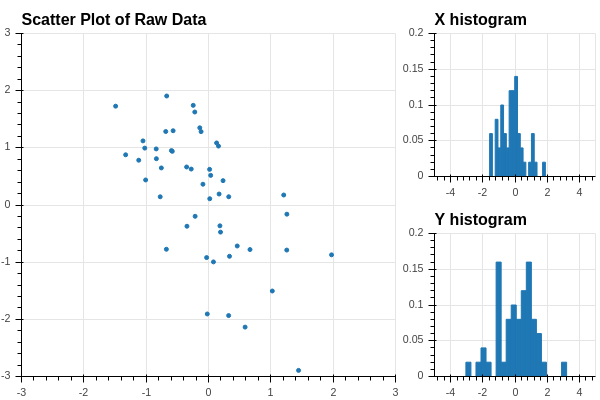
\includegraphics[width=0.5\textwidth,height=\textheight]{chapters/img/PCAsimulated-1.png}

}

\caption{\label{fig-pcasimfig}Simulated Data with Two Features}

\end{figure}

How can we get a better grip on our data in this situation? We can try
to find a ``direction'' in our data that better illuminates the
variation of the data. For example, suppose that we pick a unit vector
at the origin pointing in a particular direction in our data. See
Figure~\ref{fig-pcasimfig-1}.

\begin{figure}

{\centering 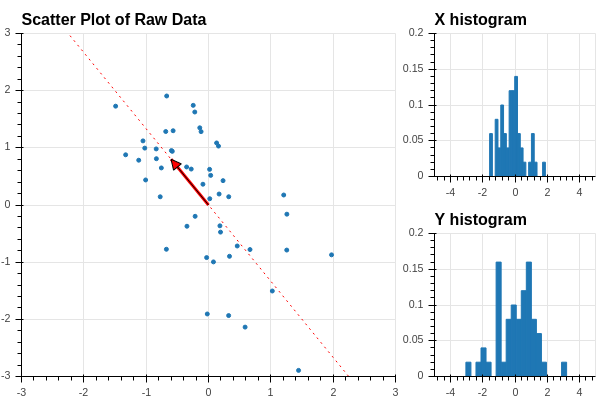
\includegraphics[width=0.5\textwidth,height=\textheight]{chapters/img/PCAsimulated-2.png}

}

\caption{\label{fig-pcasimfig-1}A direction in the data}

\end{figure}

Now we can orthogonally project the datapoints onto the line defined by
this vector, as shown in Figure~\ref{fig-pcasimfig-2}.

\begin{figure}

{\centering 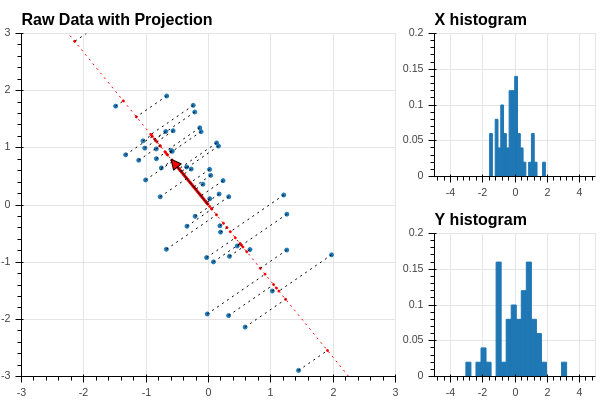
\includegraphics[width=0.5\textwidth,height=\textheight]{chapters/img/PCAsimulated-3.png}

}

\caption{\label{fig-pcasimfig-2}Projecting the datapoints}

\end{figure}

Recall that if the unit vector is defined by coordinates
\(u=[u_0,u_1]\), then the orthogonal projection of the point \(x\) with
coordinates \((x_0,x_1)\) is \((x\cdot u)u\). Now \[
x\cdot u = u_0 x_0 + u_1 x_1
\] so the coordinates of the points along the line defined by \(u\) are
the values of the score \(Z\) defined by \(u=[u_0,u_1]\). Using our work
in the previous section, we see that we can find all of these
coordinates by matrix multiplication: \[
Z = X_0 u
\] where \(X_0\) is our data matrix. Now let's add a histogram of the
values of \(Z\) to our picture:

\begin{figure}

{\centering 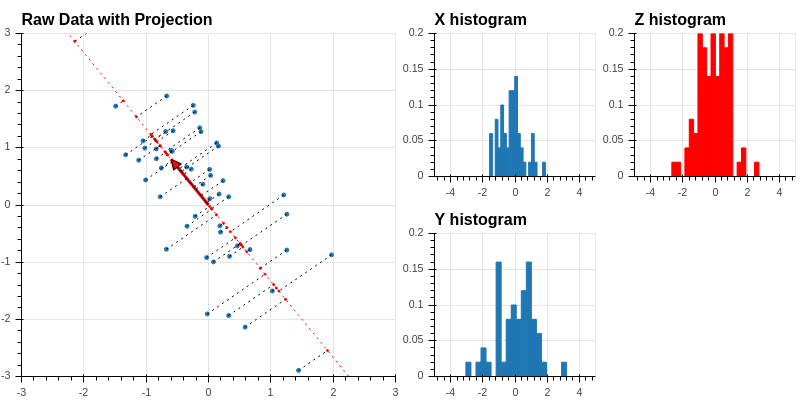
\includegraphics[width=0.5\textwidth,height=\textheight]{chapters/img/PCAsimulated-4.png}

}

\caption{\label{fig-pcasimfig-3}Distribution of Z}

\end{figure}

This histogram shows the distribution of the values of \(Z\) along the
tilted line defined by the unit vector \(u\).

Finally, using our work on the covariance matrix, we see that the
variance of \(Z\) is given by \[
\sigma_{Z}^2 = \frac{1}{50}u^{\intercal}X_{0}^{\intercal}X_{0}u = u^{\intercal}D_{0}u
\] where \(D_{0}\) is the covariance matrix of the data \(X_{0}\).

\textbf{Lemma:} Let \(X_{0}\) be a \(N\times k\) centered data matrix,
and let \(D_{0}=\frac{1}{N}X_{0}^{\intercal}X_{0}\) be the associated
covariance matrix. Let \(u\) be a unit vector in ``feature space''
\(\mathbf{R}^{k}\). Then the score \(S=X_{0}u\) can be interpreted as
the coordinates of the points of \(X_{0}\) projected onto the line
generated by \(u\). The variance of this score is \[
\sigma^{2}_{S} = u^{\intercal}D_{0}u = \sum_{i=1}^{N} s_{i}^2
\] where \(s_{i} = X_{0}[i,:]u\) is the dot product of the \(i^{th}\)
row \(X_{0}[i,:]\) with \(u\). It measures the variability in the data
``in the direction of the unit vector \(u\)''.

\hypertarget{principal-components}{%
\section{Principal Components}\label{principal-components}}

\hypertarget{change-of-variance-with-direction}{%
\subsection{Change of variance with
direction}\label{change-of-variance-with-direction}}

As we've seen in the previous section, if we choose a unit vector \(u\)
in the feature space and find the projection \(X_{0}u\) of our data onto
the line through \(u\), we get a ``score'' that we can use to measure
the variance of the data in the direction of \(u\). What happens as we
vary \(u\)?

To study this question, let's continue with our simulated data from the
previous section, and introduce a unit vector \[
u(\theta) = \left[\begin{matrix} \cos(\theta) & \sin(\theta)\end{matrix}\right].
\] This is in fact a unit vector, since
\(\sin^2(\theta)+\cos^2(\theta)=1\), and it is oriented at an angle
\(\theta\) from the \(x\)-axis.

The variance of the data in the direction of \(u(\theta)\) is given by
\[
\sigma_{\theta}^2 = u(\theta)^{\intercal}D_{0}u(\theta).
\]

A plot of this function for the data we have been considering is in
Figure~\ref{fig-pcatheta}. As you can see, the variance goes through two
full periods with the angle, and it reaches a maximum and minimum value
at intervals of \(\pi/2\) -- so the two angles where the variance are
maximum and minimum are orthogonal to one another.

\begin{figure}

{\centering 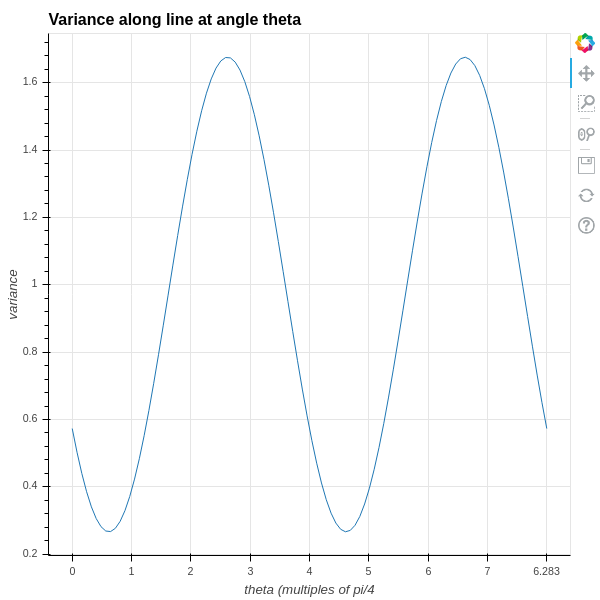
\includegraphics[width=0.25\textwidth,height=\textheight]{chapters/img/PCAtheta.png}

}

\caption{\label{fig-pcatheta}Change of variance with angle theta}

\end{figure}

The two directions where the variance is maximum and minimum are drawn
on the original data scatter plot in Figure~\ref{fig-pcaprincipal} .

\begin{figure}

{\centering 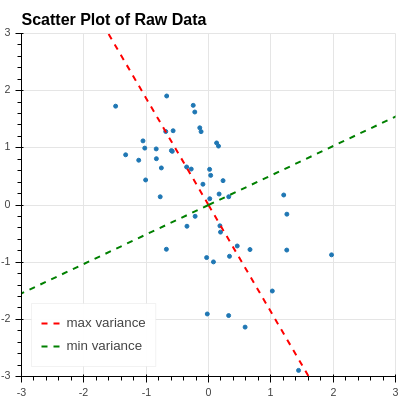
\includegraphics[width=0.25\textwidth,height=\textheight]{chapters/img/PCAprincipal.png}

}

\caption{\label{fig-pcaprincipal}Data with principal directions}

\end{figure}

Let's try to understand why this is happening.

\hypertarget{sec-extremalvariance}{%
\subsection{Directions of extremal
variance}\label{sec-extremalvariance}}

Given our centered, \(N\times i\) data matrix \(X_{0}\), with its
associated covariance matrix
\(D_{0}=\frac{1}{N}X_{0}^{\intercal}X_{0}\), we would like to find unit
vectors \(u\) in \(\mathbf{R}^{k}\) so that \[
\sigma_{u}^{2} = u^{\intercal}D_{0}u
\] reaches its maximum and its minimum. Here \(\sigma_{u}^2\) is the
variance of the ``linear score'' \(X_{0}u\) and it represents how
dispersed the data is in the ``u direction'' in \(\mathbf{R}^{k}\).

In this problem, remember that the coordinates of
\(u=(u_1,\ldots, u_{k})\) are the variables and the symmetric matrix
\(D_{0}\) is given. As usual, we to find the maximum and minimum values
of \(\sigma_{u}^{2}\), we should look at the partial derivatives of
\(\sigma_{u}^{2}\) with respect to the variables \(u_{i}\) and set them
to zero. Here, however, there is a catch -- we want to restrict \(u\) to
being a unit vector, with \(u\cdot u =\sum u_{i}^2=1\).

So this is a \emph{constrained optimization problem}:

\begin{itemize}
\tightlist
\item
  Find extreme values of the function \[
  \sigma_{u}^{2} = u^{\intercal}D_{0}u
  \]
\item
  Subject to the constraint \(\|u\|^2 = u\cdot u=1\) (or
  \(u\cdot u-1=0\))
\end{itemize}

We will use the technique of \emph{Lagrange Multipliers} to solve such a
problem.

To apply this method, we introduce the function

\begin{equation}\protect\hypertarget{eq-lagrange}{}{
S(u, \lambda) = u^{\intercal}D_{0}u - \lambda(u\cdot u -1)
}\label{eq-lagrange}\end{equation}

Then we compute the gradient

\begin{equation}\protect\hypertarget{eq-lagrangegradient}{}{
\nabla S = \left[\begin{matrix} \frac{\partial S}{\partial u_{1}} \\ \vdots \\ \frac{\partial S}{\partial u_{k}} \\ \frac{\partial S}{\partial \lambda}\end{matrix}\right]
}\label{eq-lagrangegradient}\end{equation}

and solve the system of equations \(\nabla S=0\). Here we have written
the gradient as a column vector for reasons that will become clearer
shortly.

Computing all of these partial derivatives looks messy, but actually if
we take advantage of matrix algebra it's not too bad. The following two
lemmas explain how to do this.

\textbf{Lemma}: Let \(M\) be a \(N\times k\) matrix with constant
coefficients and let \(u\) be a \(k\times 1\) column vector whose
entries are \(u_1,\ldots u_{k}\). The function \(F(u) = Mu\) is a linear
map from \(\mathbf{R}^{k}\to\mathbf{R}^{N}\). Its (total) derivative is
a linear map between the same vector spaces, and satisfies \[
D(F)(v) = Mv
\] for any \(k\times 1\) vector \(v\). If \(u\) is a \(1\times N\)
matrix, and \(G(u) = uM\), then \[
D(G)(v) = vM
\]

for any \(1\times N\) vector \(v\). (This is the matrix version of the
derivative rule that \(\frac{d}{dx}(ax)=a\) for a constant \(a\).)

\textbf{Proof:} Since \(F:\mathbf{R}^{k}\to\mathbf{R}^{N}\), we can
write out \(F\) in more traditional function notation as \[
F(u) = (F_{1}(u_1,\ldots, u_k), \ldots, F_{N}(u_1,\ldots, u_{k})
\] where \[
F_{i}(u_1,\ldots u_k) = \sum_{j=1}^{k} m_{ij}u_{j}.
\] Thus \(\frac{\partial F_{i}}{\partial u_{j}} = m_{ij}\). The total
derivative \(D(F)\) is the linear map with matrix \[
D(F)_{ij} = \frac{\partial F_{i}}{\partial u_{j}} = m_{ij}
\] and so \(D(F)=M\).

The other result is proved the same way.

\textbf{Lemma}: Let \(D\) be a symmetric \(k\times k\) matrix with
constant entries and let \(u\) be an \(k\times 1\) column vector of
variables \(u_{1},\ldots, u_{k}\). Let \(F:\mathbf{R}^{k}\to R\) be the
function \(F(u) = u^{\intercal}Du\). Then the gradient \(\nabla_{u} F\)
is a vector field -- that is, a vector-valued function of \(u\), and is
given by the formula \[
\nabla_{u} F = 2Du
\]

\textbf{Proof:} Let \(d_{ij}\) be the \(i,j\) entry of \(D\). We can
write out the function \(F\) to obtain \[
F(u_1,\ldots, u_{k}) = \sum_{i=1}^{k} \sum_{j=1}^{k} u_i d_{ij} u_j.
\] Now \(\frac{\partial F}{\partial u_{i}}\) is going to pick out only
terms where \(u_{i}\) appears, yielding: \[
\frac{\partial F}{\partial u_{i}} = \sum_{j=1}^{k} d_{ij}u_{j} + \sum_{j=1}^{k} u_{j}d_{ji}
\] Here the first sum catches all of the terms where the first ``u'' is
\(u_{i}\); and the second sum catches all the terms where the second
``u'' is \(u_{i}\). The diagonal terms \(u_{i}^2d_{ii}\) contribute once
to each sum, which is consistent with the rule that the derivative of
\(u_{i}^2d_{ii} = 2u_{i}d_{ii}\). To finish the proof, notice that \[
\sum_{j=1}^{k} u_{j}d_{ji} = \sum_{j=1}^{k} d_{ij}u_{j}
\] since \(D\) is symmetric, so in fact the two terms are the same Thus
\[
\df{u_{i}}F = 2\sum_{j=1}^{k} d_{ij}u_{j}
\] But the right hand side of this equation is twice the \(i^{th}\)
entry of \(Du\), so putting the results together we get \[
\nabla_{u}F = \left[\begin{matrix} \frac{\partial F}{\partial u_{1}} \\ \vdots \\ \frac{\partial F}{\partial u_{k}}\end{matrix}\right] = 2Du.
\]

The following theorem puts all of this work together to reduce our
questions about how variance changes with direction.

\hypertarget{sec-critvals}{%
\subsection{Critical values of the variance}\label{sec-critvals}}

\textbf{Theorem:} The critical values of the variance \(\sigma_{u}^2\),
as \(u\) varies over unit vectors in \(\mathbf{R}^{N}\), are the
eigenvalues \(\lambda_{1},\ldots,\lambda_{k}\) of the covariance matrix
\(D\), and if \(e_{i}\) is a unit eigenvector corresponding to
\(\lambda_{i}\), then \(\sigma_{e_{i}}^2 = \lambda_{i}\).

\textbf{Proof:} Recall that we introduced the Lagrange function
\(S(u,\lambda)\), whose critical points give us the solutions to our
constrained optimization problem. As we said in
Equation~\ref{eq-lagrange}: \[
S(u,\lambda) = u^{\intercal}D_{0}u - \lambda(u\cdot u - 1) = u^{\intercal}D_{0}u -\lambda(u\cdot u) + \lambda
\] Now apply our Matrix calculus lemmas. First, let's treat \(\lambda\)
as a constant and focus on the \(u\) variables. We can write
\(u\cdot u = u^{\intercal} I_{N} u\) where \(I_{N}\) is the identity
matrix to compute: \[
\nabla_{u} S = 2D_{0}u -2\lambda u
\] For \(\lambda\) we have \[
\df{\lambda}S = -u\cdot u +1.
\] The critical points occur when \[
\nabla_{u} S = 2(D_{0}-\lambda)u = 0
\] and \[
\df{\lambda}S = 1-u\cdot u = 0
\] The first equation says that \(\lambda\) must be an eigenvalue, and
\(u\) an eigenvector: \[
D_{0}u = \lambda u
\] while the second says \(u\) must be a unit vector
\(u\cdot u=\|u\|^2=1\). The second part of the result follows from the
fact that if \(e_{i}\) is a unit eigenvector with eigenvalue
\(\lambda_{i}\) then \[
\sigma_{e_{i}}^2 = e_{i}^{\intercal}D_{0}e_{i} = \lambda_{i}\|e_{i}\|^2=\lambda_{i}.
\]

To really make this result pay off, we need to recall some key facts
about the eigenvalues and eigenvectors of symmetric matrices. Because
these facts are so central to this result, and to other applications
throughout machine learning and mathematics generally, we provide proofs
in Section~\ref{sec-spectraltheorem}.

\newpage

\hypertarget{tbl-symmmat}{}
\begin{longtable}[]{@{}
  >{\raggedright\arraybackslash}p{(\columnwidth - 0\tabcolsep) * \real{1.0000}}@{}}
\caption{\label{tbl-symmmat}Properties of Eigenvalues of Real Symmetric
Matrices}\tabularnewline
\toprule()
\begin{minipage}[b]{\linewidth}\raggedright
Summary
\end{minipage} \\
\midrule()
\endfirsthead
\toprule()
\begin{minipage}[b]{\linewidth}\raggedright
Summary
\end{minipage} \\
\midrule()
\endhead
1. All of the eigenvalues \(\lambda_{1},\ldots, \lambda_{l}\) of \(D\)
are real. If \(u^{\intercal}Du\ge 0\) for all \(u\in\mathbf{R}^{k}\),
then all eigenvalues \(\lambda_{i}\) are non-negative. In the latter
case we say that \(D\) is \emph{positive semi-definite.} \\
2. If \(v\) is an eigenvector for \(D\) with eigenvalue \(\lambda\), and
\(w\) is an eigenvector with a different eigenvalue \(\lambda'\), then
\(v\) and \(w\) are orthogonal: \(v\cdot w = 0\). \\
3. There is an orthonormal basis \(u_{1},\ldots, u_{k}\) of
\(\mathbf{R}^{k}\) made up of eigenvectors of \(D\) corresponding to the
eigenvalues \(\lambda_{i}\). \\
4. Let \(\Lambda\) be the diagonal matrix with entries
\(\lambda_{1},\ldots, \lambda_{N}\) and let \(P\) be the matrix whose
columns are made up of the vectors \(u_{i}\). Then
\(D = P\Lambda P^{\intercal}.\) \\
\bottomrule()
\end{longtable}

If we combine our theorem on the critical values with the spectral
theorem we get a complete picture. Let \(D_{0}\) be the covariance
matrix of our data. Since \[
\sigma_{u}^2 = u^{\intercal}D_{0}u\ge 0 \hbox{(it's a sum of squares)}
\] we know that the eigenvalues
\(\lambda_{1}\ge\lambda_{2}\ge \cdots \ge \lambda_{k}\ge 0\) are all
nonnegative. Choose a corresponding sequence \(u_{1},\ldots u_{k}\) of
orthogonal eigenvectors where all \(\|u_{i}\|^2=1\). Since the \(u_{i}\)
form a basis of \(\mathbf{R}^{N}\), any score is a linear combination of
the \(u_{i}\): \[
S = \sum_{i=1}^{k} a_{i}u_{i}.
\] Since
\(u_{i}^{\intercal}D_{0}u_{j} = \lambda_{j}u_{i}^{\intercal}u_{j} = 0\)
unless \(i=j\), in which case it is \(\lambda_{i}\), we can compute \[
\sigma_{S}^2 = \sum_{i=1}^{k} \lambda_{i}a_{i}^2,
\] and \(\|S\|^2=\sum_{i=1}^{k} a_{i}^2\) since the \(u_{i}\) are an
orthonormal set. So in these coordinates, our optimization problem is:

\begin{itemize}
\tightlist
\item
  maximize \(\sum \lambda_{i}a_{i}^2\)
\item
  subject to the constraint \(\sum a_{i}^2 = 1\).
\end{itemize}

We don't need any fancy math to see that the maximum happens when
\(a_{1}=1\) and the other \(a_{j}=0\), and in that case, the maximum is
\(\lambda_{1}\). (If \(\lambda_{1}\) occurs more than once, there may be
a whole subspace of directions where the variance is maximal).
Similarly, the minimum value is \(\lambda_{k}\) and occurs when
\(a_{k}=1\) and the others are zero.

\hypertarget{sec-subspaces}{%
\subsection{Subspaces of extremal variance}\label{sec-subspaces}}

We can generalize the idea of the variance of our data in a particular
direction to a higher dimensional version of \emph{total variance} in a
subspace. Suppose that \(E\) is a subspace of \(\mathbf{R}^{k}\) and
\(U\) is a matrix whose columns span \(E\) -- the columns of \(U\) are
the weights of a family of scores that span \(E\). The values of these
scores are \(XU\) and the covariance matrix of this projected data is
\[\frac{1}{N}U^{\intercal}X^{\intercal}XU=U^{\intercal}D_{0}U.\].

Finally, the \emph{total variance} \(\sigma_{E}^2\) of the data
projected into \(E\) is the sum of the diagonal entries of the matrix

\[
\sigma^2_{E} = \mathop{trace}(U^{\intercal}D_{0}U)
\]

Just as the variance in a given direction \(u\) depends on the scaling
of \(u\), the variance in a subspace depends on the scaling of the
columns of \(U\). To normalize this scaling, we assume that the columns
of \(U\) are an orthonormal basis of the subspace \(E\).

Now we can generalize the question asked in
Section~\ref{sec-extremalvariance} by seeking, not just a vector \(u\)
pointing in the direction of the extremal variance, but instead the
\emph{subspace} \(U_{s}\) of dimension \(s\) with the property that the
total variance of the projection of the data into \(U_{s}\) is maximal
compared to its projection into other subspaces of that dimension. This
is called a \emph{subspace of extremal variance.}

To make this concrete, suppose we consider a subspace \(E\) of
\(\mathbf{R}^{k}\) of dimension \(t\) with basis
\(w_{1},\ldots, w_{t}\). Complete this to a basis
\(w_{1},\ldots, w_{t},w_{t+1},\ldots, w_{k}\) of \(\mathbf{R}^{k}\) and
then apply the Gram Schmidt Process (see Section~\ref{sec-gsprocess}) to
find an orthonormal basis
\(w'_{1},\ldots,w'_{s},w'_{s+1},\ldots, w'_{k}\) where the
\(w'_{1},\ldots, w'_{t}\) are an orthonormal basis for \(E\). Let \(W\)
be the \(k\times t\) matrix whose columns are the \(w'_{i}\) for
\(i=1,\ldots,t\). The rows of the matrix \(X_{0}W\) given the
coordinates of the projection of each sample into the subspace \(E\)
expressed in terms of the scores corresponding to these vectors
\(w'_{i}\). The total variance of these projections is

\[
\sigma_{E}^2 = \sum_{i=1}^{t} \|X_{0}w'_{i}\|^2 = \sum_{i=1}^{t} (w'_{i})^{\intercal}X_{0}^{\intercal}X_{0}w'_{i}  = \sum_{i=1}^{t} (w'_{i})^{\intercal}D_{0}w'_{i}
\]

If we want to maximize this, we have the constrained optimization
problem of finding \(w'_{1},\ldots, w'_{t}\) so that

\begin{itemize}
\tightlist
\item
  \(\sum_{i=1}^{t} (w'_{i})^{\intercal}D_{0}w'_{i}\) is maximal
\item
  subject to the constraint that each \(w_{i}\) has \(\|w'_{i}\|^2=1\),
\item
  and that the \(w'_{i}\) are orthogonal, meaning
  \(w'_{i}\cdot w'_{j}=0\) for \(i\not=j\),
\item
  and that the \(w'_{i}\) are linearly independent.
\end{itemize}

Then the span \(E\) of these \(w'_{i}\) is subspace of extremal
variance.

\textbf{Theorem:} A \(t\)-dimensional subspace \(E\) is a subspace of
extremal variance if and only if it is spanned by \(t\) orthonormal
eigenvectors of the matrix \(D_{0}\) corresponding to the \(t\) largest
eigenvalues for \(D_{0}\).

\textbf{Proof:} We can approach this problem using Lagrange multipliers
and matrix calculus if we are careful. Our unknown is \(k\times t\)
matrix \(W\) whose columns are the \(t\) (unknown) vectors \(w'_{i}\).
The objective function that we are seeking to maximize is \[
F = \mathop{trace}(W^{\intercal}D_{0}W) = \sum_{i=1}^{t} (w'_{i})^{\intercal}D_{0}w_{i}.
\] The constraints are the requirements that \(\|w'_{i}\|^2=1\) and
\(w'_{i}\cdot w'_{j}=0\) if \(i\not=j\). If we introduction a matrix of
lagrange multipliers \(\Lambda=(\lambda_{ij})\), where \(\lambda_{ij}\)
is the multiplier that goes with the the first of these constraints when
\(i=j\), and the second when \(i\not=j\), we can express our Lagrange
function as: \[
S(W,\Lambda) = \mathop{trace}(W^{\intercal}D_{0}W) - (W^{\intercal}W-I)\Lambda
\] where \(I\) is the \(t\times t\) identity matrix.

Taking the derivatives with respect to the entries of \(W\) and of
\(\Lambda\) yields the following two equations: \begin{align*}
D_{0}W &= W\Lambda \\
W^{\intercal}W &= I \\
\end{align*}

The first of these equations says that the space \(E\) spanned by the
columns of \(W\) is \emph{invariant} under \(D_{0}\), while the second
says that the columns of \(W\) form an orthonormal basis.

Let's assume for the moment that we have a matrix \(W\) that satisfies
these conditions.\\
Then it must be the case that \(\Lambda\) is a symmetric, real valued
\(t\times t\) matrix, since \[
W^{\intercal}D_{0}W = W^{\intercal}W\Lambda = \Lambda.
\] and the matrix on the left is symmetric.

By the properties of real symmetric matrices (the spectral theorem),
there are orthonormal vectors \(q_{1},\ldots q_{t}\) that are
eigenvectors of \(\Lambda\) with corresponding eigenvalues \(\tau_{i}\).
If we let \(Q\) be the matrix whose columns are the vectors \(q_{i}\)
and let \(T\) be the diagonal \(t\times t\) matrix whose entries are the
\(\tau_{i}\), we have \[
\Lambda Q = QT.
\]

If we go back to our original equations, we see that if \(W\) exists
such that \(DW=W\Lambda\), then there is a matrix \(Q\) with orthonormal
columns and a diagonal matrix \(T\) such that \[
D_{0}WQ = W\Lambda Q = W Q T.
\] In other words, \(WQ\) is a matrix whose columns are eigenvectors of
\(D_{0}\) with eigenvalues \(\tau_{i}\) for \(i=1,\ldots, t\).

Thus we see how to construct an invariant subspace \(E\) and a solution
matrix \(W\). Such an \(E\) is spanned by \(t\) orthonormal eigenvectors
\(q_{i}\) with eigenvalues \(\tau_{i}\) of \(D_{0}\); and \(W\) is is
the matrix whose columns are the \(q_{i}\). Further, in that case, the
total variance associated to \(E\) is the sum of the eigenvalues
\(\tau_{i}\); to make this as large as possible, we should choose our
eigenvectors to correspond to \(t\) of the largest eigenvalues of
\(D_{0}\). This concludes the proof.

\hypertarget{definition-of-principal-components}{%
\subsection{Definition of Principal
Components}\label{definition-of-principal-components}}

\textbf{Definition:} The orthonormal unit eigenvectors \(u_{i}\) for
\(D_{0}\) are the \emph{principal directions} or \emph{principal
components} for the data \(X_{0}\).

\textbf{Theorem:} The maximum variance occurs in the principal
direction(s) associated to the largest eigenvalue, and the minimum
variance in the principal direction(s) associated with the smallest one.
The covariance between scores in principal directions associatedwith
different eigenvalues is zero.

At this point, the picture in Figure~\ref{fig-pcaprincipal} makes sense
-- the red and green dashed lines are the principal directions, they are
orthogonal to one another, and the point in the directions where the
data is most (and least) ``spread out.''

\textbf{Proof:} The statement about the largest and smallest eigenvalues
is proved at the very end of the last section. The covariance of two
scores corresponding to different eigenvectors \(u_{i}\) and \(u_{j}\)
is \[u_{i}^{\intercal}D_{0}u_{j} = \lambda_{j}(u_{i}\cdot u_{j}) = 0\]
since the \(u_{i}\) and \(u_{j}\) are orthogonal.

Sometimes the results above are presented in a slightly different form,
and may be referred to, in part, as Rayleigh's theorem.

\textbf{Corollary:} (Rayleigh's Theorem) Let \(D\) be a real symmetric
matrix and let \[
H(v) = \max_{v\not = 0}\frac{v^{\intercal}Dv}{v^{\intercal}v}.
\] Then \(H(v)\) is the largest eigenvalue of \(D\). (Similarly, if we
replace \(\max\) by \(\min\), then the minimum is the least eigenvalue).

\textbf{Proof:} The maximum of the function \(H(v)\) is the solution to
the same optimization problem that we considered above.

\textbf{Exercises.}

\begin{enumerate}
\def\labelenumi{\arabic{enumi}.}
\item
  Prove that the two expressions for \(\sigma_{X}^2\) given in
  Equation~\ref{eq-variance} are the same.
\item
  Prove that the covariance matrix is as described in the proposition in
  Section~\ref{sec-covarmat}.
\item
  Let \(X_{0}\) be a \(k\times N\) matrix with entries \(x_{ij}\) for
  \(1\le i\le k\) and \(1\le j\le N\). If a linear score is defined by
  the constants \(a_{1},\ldots a_{N}\), check that equation
  Equation~\ref{eq-linearscore} holds as claimed.
\item
  Why is it important to use a unit vector when computing the variance
  of \(X_{0}\) in the direction of \(u\)? Suppose \(v=\lambda u\) where
  \(u\) is a unit vector and \(\lambda>0\) is a constant. Let \(S'\) be
  the score \(X_{0}v\). How is the variance of \(S'\) related to that of
  \(S=X_{0}u\)?
\end{enumerate}

\hypertarget{dimensionality-reduction-via-principal-components}{%
\section{Dimensionality Reduction via Principal
Components}\label{dimensionality-reduction-via-principal-components}}

The principal components associated with a dataset separate out
directions in the feature space in which the data is most (or least)
variable. One of the main applications of this information is to enable
us to take data with a great many features -- a set of points in a high
dimensional space -- and, by focusing our attention on the scores
corresponding to the principal directions, capture most of the
information in the data in a much lower dimensional setting.

To illustrate how this is done, let \(X\) be a \(N\times k\) data
matrix, let \(X_{0}\) be its centered version, and let
\(D_{0} = \frac{1}{N}X_{0}^{\intercal}X\) be the associated covariance
matrix.

Apply the spectral theorem (proved in Section~\ref{sec-spectraltheorem})
to the covariance matrix to obtain eigenvalues
\(\lambda_{1}\ge \lambda_{2}\ge\cdots \lambda_{k}\ge 0\) and associated
eigenvectors \(u_{1},\ldots, u_{k}\). The scores \(S_{i}=X_{0}u_{i}\)
give the values of the data in the principal directions. The variance of
\(S_{i}\) is \(\lambda_{i}\).

Now choose a number \(t<k\) and consider the vectors
\(S_{1},\ldots, S_{t}\). The \(j^{th}\) entry in \(S_{i}\) is the value
of the score \(S_{i}\) for the \(j^{th}\) data point. Because
\(S_{1},\ldots, S_{t}\) capture the most significant variability in the
original data, we can learn a lot about our data by considering just
these \(t\) features of the data, instead of needing all \(N\).

To illustrate, let's look at an example. We begin with a synthetic
dataset \(X_{0}\) which has \(200\) samples and \(15\) features. The
data (some of it) for some of the samples is shown in
Table~\ref{tbl-rawdata}.

\hypertarget{tbl-rawdata}{}
\begin{longtable}[]{@{}llllllllllll@{}}
\caption{\label{tbl-rawdata}Simulated Data for PCA
Analysis}\tabularnewline
\toprule()
& f-0 & f-1 & f-2 & f-3 & f-4 & ... & f-10 & f-11 & f-12 & f-13 &
f-14 \\
\midrule()
\endfirsthead
\toprule()
& f-0 & f-1 & f-2 & f-3 & f-4 & ... & f-10 & f-11 & f-12 & f-13 &
f-14 \\
\midrule()
\endhead
s-0 & 1.18 & -0.41 & 2.02 & 0.44 & 2.24 & ... & 0.32 & 0.95 & 0.88 &
1.10 & 0.89 \\
s-1 & 0.74 & 0.58 & 1.54 & 0.23 & 2.05 & ... & 0.99 & 1.14 & 1.56 & 0.99
& 0.59 \\
... & ... & ... & ... & ... & ... & ... & ... & ... & ... & ... & ... \\
s-198 & 1.04 & 2.02 & 1.44 & 0.40 & 1.33 & ... & 0.62 & 0.62 & 0.54 &
1.96 & 0.04 \\
s-199 & 0.92 & 2.09 & 1.58 & 1.19 & 1.17 & ... & 0.42 & 0.85 & 0.83 &
2.22 & 0.90 \\
\bottomrule()
\end{longtable}

The full dataset is a \(200\times 15\) matrix; it has \(3000\) numbers
in it and we're not really equipped to make sense of it. We could try
some graphing -- for example, Figure~\ref{fig-features} shows a scatter
plot of two of the features plotted against each other.

\begin{figure}

{\centering 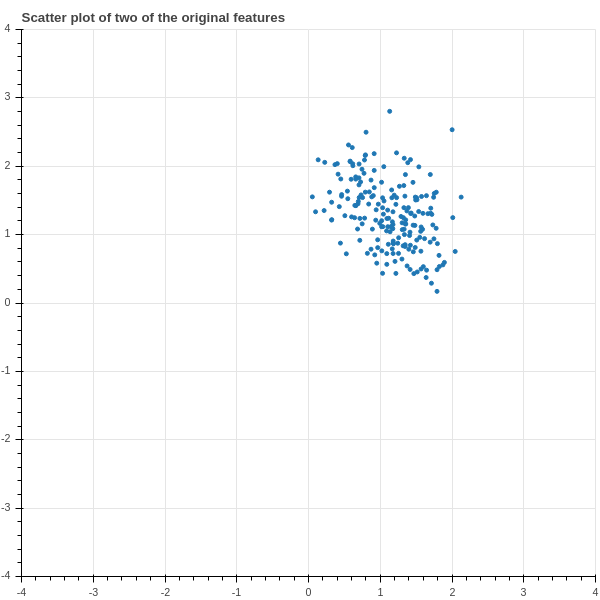
\includegraphics[width=0.5\textwidth,height=\textheight]{chapters/img/features.png}

}

\caption{\label{fig-features}Scatter Plot of Two Features}

\end{figure}

Unfortunately there's not much to see in Figure~\ref{fig-features} --
just a blob -- because the individual features of the data don't tell us
much in isolation, whatever structure there is in this data arises out
of the relationship between different features.

In Figure~\ref{fig-densitygrid} we show a ``density grid'' plot of the
data. The graph in position \(i,j\) shows a scatter plot of the
\(i^{th}\) and \(j^{th}\) columns of the data, except in the diagonal
positions, where in position \(i,i\) we plot a histogram of column
\(i\). There's not much structure visible; it is a lot of blobs.

\begin{figure}

{\centering 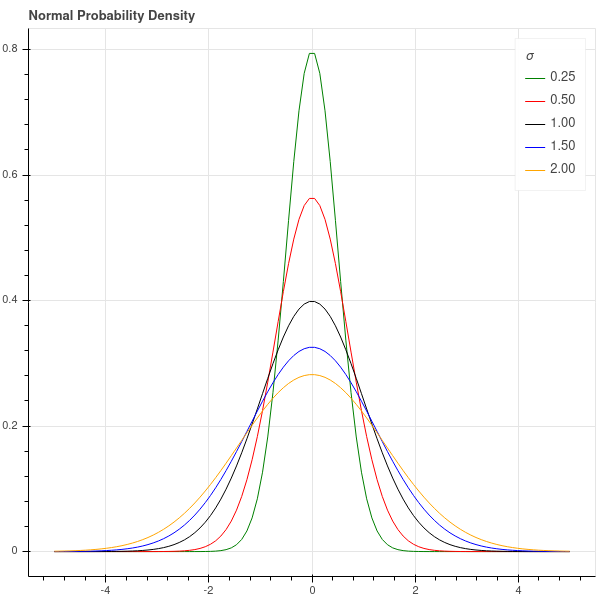
\includegraphics[width=0.5\textwidth,height=\textheight]{chapters/img/density.png}

}

\caption{\label{fig-densitygrid}Density Grid Plot of All Features}

\end{figure}

So let's apply the theory of principal components. We use a software
package to compute the eigenvalues and eigenvectors of the matrix
\(D_{0}\). The \(15\) eigenvalues
\(\lambda_{1}\ge \cdots \ge \lambda_{15}\) are plotted, in descending
order, in Figure~\ref{fig-eigenvalues} .

\begin{figure}

{\centering 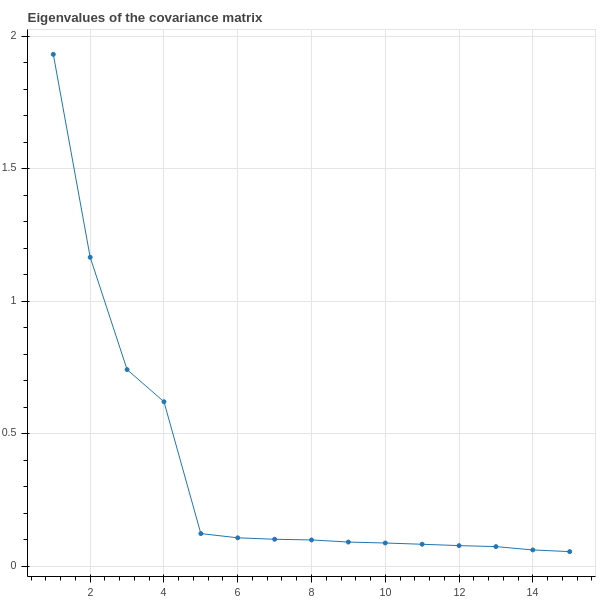
\includegraphics[width=0.5\textwidth,height=\textheight]{chapters/img/eigenvalues.png}

}

\caption{\label{fig-eigenvalues}Eigenvalues of the Covariance Matrix}

\end{figure}

This plot shows that the first \(4\) eigenvalues are relatively large,
while the remaining \(11\) are smaller and not much different from each
other. We interpret this as saying that \emph{most of the variation in
the data is accounted for by the first four principal components.} We
can even make this quantitative. The \emph{total variance} of the data
is the sum of the eigenvalues of the covariance matrix -- the trace of
\(D_{0}\) -- and in this example that sum is around \(5\). The sum of
the first \(4\) eigenvalues is about \(4\), so the first four eignvalues
account for about \(4/5\) of the total variance, or about \(80\%\) of
the variation of the data.

Now let's focus in on the two largest eigenvalues \(\lambda_{1}\) and
\(\lambda_{2}\) and their corresponding eigenvectors \(u_{1}\) and
\(u_{2}\). The \(200\times 1\) column vectors \(S_{1}=X_{0}u_{1}\) and
\(S_{2}=X_{0}u_{2}\) are the values of the scores associated with these
two eigenvectors. So for each data point (each row of \(X_{0}\)) we have
two values (the corresponding entries of \(S_{1}\) and \(S_{2}\).) In
Figure~\ref{fig-principalvalues} we show a scatter plot of these scores.

\begin{figure}

{\centering 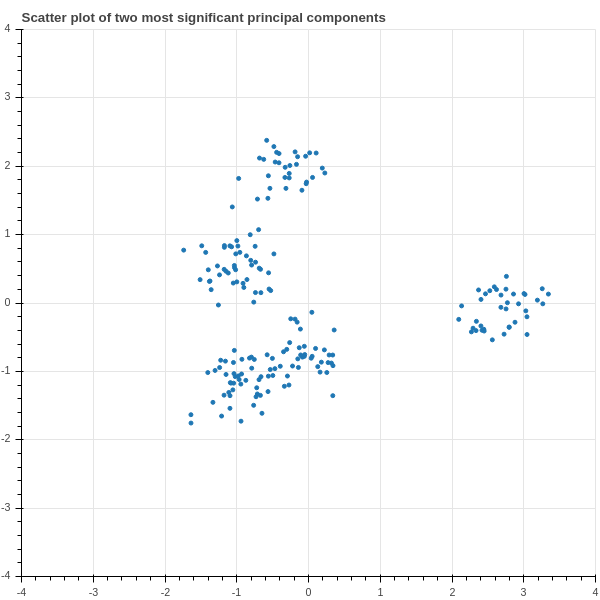
\includegraphics[width=0.5\textwidth,height=\textheight]{chapters/img/pcadimred.png}

}

\caption{\label{fig-principalvalues}Scatter Plot of Scores in the First
Two Principal Directions}

\end{figure}

Notice that suddenly some structure emerges in our data! We can see that
the 200 points are separated into five clusters, distinguished by the
values of their scores! This ability to find hidden structure in
complicated data, is one of the most important applications of principal
components.

If we were dealing with real data, we would now want to investigate the
different groups of points to see if we can understand what
characteristics the principal components have identified.

\hypertarget{loadings}{%
\subsection{Loadings}\label{loadings}}

There's one last piece of the PCA puzzle that we are going to
investigate. In Figure~\ref{fig-principalvalues}, we plotted our data
points in the coordinates given by the first two principal components.
In geometric terms, we took the cloud of \(200\) points in
\(\mathbf{R}^{15}\) given by the rows of \(X_{0}\) and projected those
points into the two dimensional plane spanned by the eigenvectors
\(u_{1}\) and \(u_{2}\), and then plotted the distribution of the points
in that plane.

More generally, suppose we take our dataset \(X_{0}\) and consider the
first \(t\) principal components corresponding to the eigenvectors
\(u_{1},\ldots, u_{t}\). The projection of the data into the space
spanned by these eigenvectors is the represented by the
\(S = k\times t\) matrix \(X_{0}U\) where \(U\) is the \(k\times t\)
matrix whose columns are the eigenvectors \(u_{i}\). Each row of \(S\)
gives the values of the score arising from \(u_{i}\) in the \(i^{th}\)
column for \(i=1,\ldots, t\).

The remaining question that we wish to consider is: how can we see some
evidence of the original features in subspace? We can answer this by
imagining that we had an artificial sample \(x\) that has a measurement
of \(1\) for the \(i^{th}\) feature and a measurement of zero for all
the other features. The corresponding point is represented by a
\(1\times k\) row vector with a \(1\) in position \(i\). The projection
of this synthetic sample into the span of the first \(t\) principal
components is the \(1\times t\) vector \(xU\). Notice, however, that
\(xU\) is just the \(i^{th}\) row of the matrix \(U\). This vector in
the space spanned by the \(u_{i}\) is called the ``loading'' of the
\(i^{th}\) feature in the principal components.

This is illustrated in Figure~\ref{fig-loadings}, which shows a line
along the direction of the loading corresponding to the each feature
added to the scatter plot of the data in the plane spanned by the first
two principal components. One observation one can make is that some of
the features are more ``left to right'', like features \(7\) and \(8\),
while others are more ``top to bottom'', like \(6\). So points that lie
on the left side of the plot have smaller values of features \(7\) and
\(8\), while those at the top of the plot have larger values of feature
\(6\).

\begin{figure}

{\centering 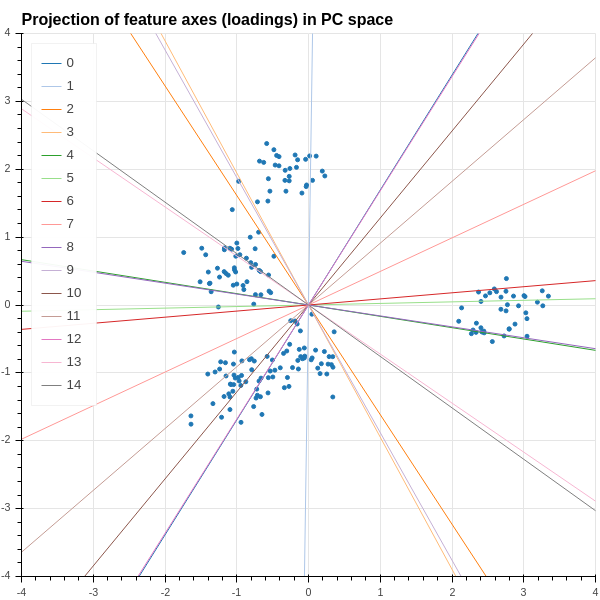
\includegraphics[width=0.5\textwidth,height=\textheight]{chapters/img/loading.png}

}

\caption{\label{fig-loadings}Loadings in the Principal Component Plane}

\end{figure}

\hypertarget{sec-svd}{%
\subsection{The singular value decomposition}\label{sec-svd}}

The singular value decomposition is a slightly more detailed way of
looking at principal components. Let \(\Lambda\) be the diagonal matrix
of eigenvalues of \(D_{0}\) and let \(P\) be the \(k\times k\)
orthogonal matrix whose columns are the principal components. Then we
have \[
D_{0} =\frac{1}{N}X_{0}^{\intercal}X_{0}= P\Lambda P^{\intercal}.
\] Consider the \(N\times k\) matrix \[
X_{0}P = A.
\]

As we saw in the previous section, the columns of \(A\) give the
projection of the data into the \(k\) principal directions. Then

\[A^{\intercal}A=P^{\intercal}X_{0}^{\intercal}X_{0}P=N\Lambda.\]

In other words, the columns of \(A\) are orthogonal and the diagonal
entries of \(A^{\intercal}A\) are \(N\) times the variance of the data
in the various principal directions.

Now we are going to tinker with the matrix \(A\) in order to make an
\(N\times N\) orthogonal matrix. The first modification we make is to
normalize the columns of \(A\) so that they have length \(1\). We do
this by setting \[
A_{1} = A(N\Lambda)^{-1/2}.
\] Then \(A_{1}^{\intercal}A_{1}\) is the identity, so the columns of
\(A_{1}\) are orthonormal. Here we are assuming that the eigenvalues of
\(D_{0}\) are nonzero -- this isn't strictly necessary, and we could
work around this, but for simplicity we will assume it's true. It
amounts to the assumption that the independent variables are not
linearly related, as we've seen before.

The second modification is to extend \(A_{1}\) to an \(N\times N\)
matrix. The \(k\) columns of \(A_1\) span only a \(k\)-dimensional
subspace of the \(N\)-dimensional space where the feature vectors lie.\\
Complete the subspace by finding an orthogonal complement to it -- that
is, find \(N-k\) mutually orthogonal unit vectors all orthogonal to the
column space of \(A_1\). By adding these vectors to \(A\) as columns,
create an extended \(N\times N\) matrix \(\tilde{A}_1\) which is
orthogonal.

Notice that \(\tilde{A}_{1}^{\intercal}A\) is an \(N\times k\) matrix
whose upper \(k\times k\) block is \((N\Lambda)^{1/2}\) and whose final
\(N-k\) rows are all zero. We call this matrix \(\tilde{\Lambda}\).

To maintain consistency with the traditional formulation, we let
\(U=\tilde{A}_{1}^{\intercal}\) and then we have the following
proposition.

\textbf{Proposition:} We have a factorization
\begin{equation}\protect\hypertarget{eq-svd}{}{
X_{0} = U\tilde{\Lambda}P^{\intercal}
}\label{eq-svd}\end{equation} where \(U\) and \(P\) are orthogonal
matrices of size \(N\times N\) and \(k\times k\) respectively, and
\(\tilde{\Lambda}\) is an \(N\times k\) diagonal matrix. This is called
the ``singular value decomposition'' of \(X_{0}\), and the entries of
\(\tilde{\Lambda}\) are called the singular values. If we let
\(u_1,\ldots, u_k\) be the first \(k\) rows of \(U\), then the \(k\)
column vectors \(u_{i}^{\intercal}\) are an orthonormal basis for the
feature space spanned by the columns of \(X_{0}\), and they point in the
``principal directions'' for the data matrix \(X_{0}\).

In this section we take a slight detour and apply what we've learned
about the covariance matrix, principal components, and the singular
value decomposition to the original problem of linear regression that we
studied in Chapter 1.

In this setting, in addition to our centered data matrix \(X_{0}\), we
have a vector \(Y\) of target values and we find the ``best''
approximation \[
\hat{Y} = X_{0}M
\] using the least squares method. As we showed in Chapter 1, the
optimum \(M\) is found as \[
M = (X_{0}^{\intercal}X_{0})^{-1}X^{\intercal}Y = ND_{0}^{-1}X_0^{\intercal}Y
\] and the predicted values \(\hat{Y}\) are \[
\hat{Y} = NX_{0}D_{0}^{-1}X_0^{\intercal}Y.
\]

Geometrically, we understood this process as defining \(\hat{Y}\) to be
the orthogonal projection of \(Y\) into the subspace spanned by the
columns of \(X_{0}\).

Let's use the decomposition (see Equation~\ref{eq-svd} )
\(X_{0}=U\tilde{\Lambda}P^{\intercal}\) in this formula. First, notice
that \[
X_{0}^{\intercal}X_{0}= P\tilde{\Lambda}^{\intercal}U^{\intercal}U\tilde{\Lambda}P^{\intercal} = P\tilde{\Lambda}^{\intercal}\tilde{\Lambda}P^{\intercal}.
\]

The middle term \(\tilde{\Lambda}^{\intercal}\tilde{\Lambda}\) is the
\(k\times k\) matrix \(\Lambda\) whose diagonal entries are
\(N\lambda_{i}\) where \(\lambda_{i}\) are the eigenvalues of the
covariance matrix \(D_{0}\). Assuming these are all nonzero (which is
tantamount to the assumption that the covariance matrix is invertible),
we obtain \[
\hat{Y} = NU\tilde{\Lambda}P^{\intercal}P\Lambda^{-1}P^{\intercal}P\tilde{\Lambda}^{\intercal}U^{\intercal}Y.
\] There is a lot of cancellation here, and in the end what's left is \[
\hat{Y}=UEU^{\intercal}Y
\] where \(E\) is and \(N\times N\) matrix whose upper \(k\times k\)
block is the identity and whose remaining entries are zero. Rearranging
a bit more we have \[
U^{\intercal}\hat{Y} = EU^{\intercal}Y.
\]

To unpack this equation, let \(u_{1},\ldots, u_{N}\) be the rows of the
matrix \(U\). Since \(U\) is an orthogonal matrix, the column vectors
\(u_{i}^{\intercal}\) are an orthonormal basis for the \(N\) dimensional
space where the columns of \(X_{0}\) lie. We can write the target vector
\(Y\) \[
Y = \sum_{j=1}^{N} (u_{j}\cdot Y)u_{j}^{\intercal}.
\]

Then the projection \(\hat{Y}\) of \(Y\) into the subspace spanned by
the data is obtained by dropping the last \(N-k\) terms in the sum:

\[
\hat{Y}=\sum_{j=1}^{k} (u_{j}\cdot Y)u_{j}^{\intercal}
\]

\hypertarget{sec-spectraltheorem}{%
\section{Eigenvalues and Eigenvectors of Real Symmetric Matrices (The
Spectral Theorem)}\label{sec-spectraltheorem}}

Now that we've shown how to apply the theory of eigenvalues and
eigenvectors of symmetric matrices to extract principal directions from
data, and to use those principal directions to find structure, we will
give a proof of the properties that we summarized in
Table~\ref{tbl-symmmat}.

A key tool in the proof is the Gram-Schmidt orthogonalization process.

\hypertarget{sec-gsprocess}{%
\subsection{Gram-Schmidt}\label{sec-gsprocess}}

\textbf{Proposition (Gram-Schmidt Process):} Let \(w_{1},\ldots, w_{k}\)
be a collection of linearly independent vectors in \(\mathbf{R}^{N}\)
and let \(W\) be the span of the \(w_{i}\). Let \(u_{1} = w_{1}\) and
let \[
u_{i} = w_{i} - \sum_{j=1}^{i-1} \frac{w_{i}\cdot u_{j}}{u_{j}\cdot u_{j}}u_{j}
\] for \(i=2,\ldots, k\). Then

\begin{itemize}
\tightlist
\item
  The vectors \(u_{i}\) are orthogonal: \(u_{i}\cdot u_{j}=0\) unless
  \(i=j\).
\item
  The vectors \(u_{i}\) span \(W\).
\item
  Each \(u_{i}\) is orthogonal to the all of \(w_{1},\ldots, w_{i-1}\).
\item
  The vectors \(u'_{i} = u_{i}/\|u_{i}\|\) are orthonormal.
\end{itemize}

\textbf{Proof:} This is an inductive exercise, and we leave it to you to
work out the details.

\hypertarget{the-spectral-theorem}{%
\subsection{The spectral theorem}\label{the-spectral-theorem}}

\textbf{Theorem:} Let \(D\) be a real symmetric \(N\times N\) matrix.
Then:

\begin{enumerate}
\def\labelenumi{\arabic{enumi}.}
\tightlist
\item
  All of the \(N\) eigenvalues
  \(\lambda_1\ge \lambda_2\ge \cdots \ge \lambda_{N}\) are real. If
  \(u^{\intercal}Du\ge 0\) for all \(u\in\mathbf{R}^{N}\), then all
  eigenvalues \(\lambda_{i}\ge 0\).
\item
  The matrix \(D\) is diagonalizable -- that is, it has \(N\) linearly
  independent eigenvectors.
\item
  If \(v\) and \(w\) are eigenvectors corresponding to eigenvalues
  \(\lambda\) and \(\lambda'\), with \(\lambda\not=\lambda'\), then
  \(v\) and \(w\) are orthogonal: \(v\cdot w=0\).
\item
  There is an orthonormal basis \(u_{1},\ldots, u_{N}\) of
  \(\mathbf{R}^{N}\) made up of eigenvectors for the eigenvalues
  \(\lambda_{i}\).
\item
  Let \(\Lambda\) be the diagonal matrix with entries
  \(\lambda_{1},\ldots, \lambda_{N}\) and let \(P\) be the matrix whose
  columns are made up of the eigenvectors \(u_{i}\). Then
  \(D=P\Lambda P^{\intercal}\).
\end{enumerate}

\textbf{Proof:} First of all, we use the fact that any matrix has at
least one eigenvector with associated eigenvalue. This is a theorem from
linear algebra that relies on the fundamental theorem of algebra. With
this result available, we start by proving part 1. Suppose that
\(\lambda\) is an eigenvalue of \(D\). Let \(u\) be a corresponding
nonzero eigenvector. Then \(Du=\lambda u\) and
\(D\overline{u}=\overline{\lambda}\overline{u}\), where \(\overline{u}\)
is the vector whose entries are the conjugates of the entries of \(u\)
(and \(\overline{D}=D\) since \(D\) is real). Now we have \[
\overline{u}^{\intercal}Du = \lambda \overline{u}\cdot u = \lambda\|u\|^2
\] and \[
u^{\intercal}D\overline{u} = \overline{\lambda}u\cdot \overline{u} = \overline{\lambda}\|u\|^2.
\] But the left hand side of both of these equations are the same (take
the transpose and use the symmetry of \(D\)) so we must have
\(\lambda\|u\|^2 = \overline{\lambda}\|u\|^2\) so
\(\lambda=\overline{\lambda}\), meaning \(\lambda\) is real.

If we have the additional property that \(u^{\intercal}Du\ge 0\) for all
\(u\), then in particular
\(u_{i}^{\intercal}Du_{i} = \lambda\|u\|^2\ge 0\), and since
\(\|u\|^2> 0\) we must have \(\lambda\ge 0\).

Property \(2\) is in some ways the most critical fact. We know from the
general theory of the characteristic polynomial, and the fundamental
theorem of algebra, that \(D\) has \(N\) complex eigenvalues, although
some may be repeated. However, it may not be the case that \(D\) has
\(N\) linearly independent eigenvectors -- it may not be
\emph{diagonalizable}. So we will establish that any \emph{symmetric}
matrix over the real numbers is diagonalizable.

A one-by-one matrix is automatically symmetric and diagonalizable. In
the \(N\)-dimensional case, we know, at least, that \(D\) has at least
one eigenvector, and real one at that by part \(1\), and this gives us a
place to begin an inductive argument.

Let \(v_{N}\not=0\) be an eigenvector with eigenvalue \(\lambda\) and
normalized so that \(\|v_{N}\|^2=1\),\\
and extend this to a basis \(v_{1},\ldots v_{N}\) of \(\mathbf{R}^{N}\).
Apply the Gram-Schmidt process to construct an orthonormal basis of
\(\mathbf{R}^{N}\) \(u_{1},\ldots, u_{N}\) so that \(u_{N}=v_{N}\).

Any vector \(v\in\mathbf{R}^{N}\) is a linear combination \[
v = \sum_{i=1}^{N} a_{i}u_{i}
\] and, since the \(u_{i}\) are orthonormal, the coefficients can be
calculated as \(a_{i}=(u_{i}\cdot v)\).

Using this, we can find the matrix \(D'\) of the linear map defined by
our original matrix \(D\) in this new basis. By definition, if
\(d'_{ij}\) are the entries of \(D'\), then

\[
Du_{i} = \sum_{j=1}^{N} d'_{ij} u_{j}
\]

and so

\[
d'_{ij} = u_{j}\cdot Du_{i} = u_{j}^{\intercal}Du_{i}.
\]

Since \(D\) is symmetric,
\(u_{j}^{\intercal}Du_{i} =u_{i}^{\intercal}Du_{j}\) and so
\(d'_{ij}=d'_{ji}\). In other words, the matrix \(D'\) is still
symmetric. Furthermore,

\[
d'_{Ni} = u_{i}\cdot Du_{N} = u_{i}\cdot \lambda u_{N} = \lambda (u_{i}\cdot u_{N})
\]

since \(u_{N}=v_{N}\). Since the \(u_{i}\) are an orthonormal basis, we
see that \(d'_{iN}=0\) unless \(i=N\), and \(d'_{NN}=\lambda\).

In other words, the matrix \(D'\) has a block form: \[
D' = \left(\begin{matrix} *&* & \cdots &*  & 0 \\ \vdots & \vdots & \ddots   & \vdots & \vdots \\
* & *& \cdots &*  & 0 \\
0 & 0 & \cdots &0 &\lambda \end{matrix}\right)
\] and the block denoted by \(*\)'s is symmetric. If we call that block
\(D_{*}\), the inductive hypothesis tells us that the symmetric matrix
\(D_{*}\) is diagonalizable, so it has a basis of eigenvectors
\(u'_{1},\ldots, u'_{N-1}\) with eigenvalues
\(\lambda_{1},\ldots, \lambda_{N-1}\); this gives us a basis for the
subspace of \(\mathbf{R}^{N}\) spanned by \(u_{1},\ldots, u_{N-1}\)
which, together with \(u_{N}\) gives us a basis of \(\mathbf{R}^{N}\)
consisting of eigenvectors of \(D\).

This finishes the proof of Property \(2\).

For property \(3\), compute \[
v^{\intercal}Dw = \lambda'(v\cdot w)=w^{\intercal}Dv = \lambda (w\cdot v).
\] Since \(\lambda\not=\lambda'\), we must have \(v\cdot w=0\).

For property \(4\), if the eigenvalues are all distinct, this is a
consequence of property \(2\) -- you have \(N\) eigenvectors, scaled to
length \(1\), for different eigenvalues, and by \(2\) they are
orthogonal. So the only complication is the case where some eigenvalues
are repeated. If \(\lambda\) occurs \(r\) times, then you have \(r\)
linearly independent vectors \(u_{1},\ldots, u_{r}\) that span the
\(\lambda\) eigenspace. The Gram-Schmidt process allows you to construct
an orthonormal set that spans this eigenspace, and while this
orthonormal set isn't unique, any one of them will do.

For property \(5\), let \(e_{i}\) be the column vector that is zero
except for a \(1\) in position \(i\). The product
\(e_{j}^{\intercal}De_{i}=d_{ij}\). Let's write \(e_{i}\) and \(e_{j}\)
in terms of the orthonormal basis \(u_{1},\ldots u_{N}\): \[
e_{i} = \sum_{k=1}^{N} (e_{i}\cdot u_{k})u_k \hbox{ and } e_{j} = \sum_{k=1}^{N}(e_{j}\cdot u_{k})u_{k}.
\] Using this expansion, we compute \(e_{j}^{\intercal}De_{i}\) in a
more complicated way: \[
e_{j}^{\intercal}De_{i} = \sum_{r=1}^{N}\sum_{s=1}^{N} (e_{j}\cdot u_{r})(e_{i}\cdot u_{s})(u_{r}^{\intercal}Du_{s}).
\] But \(u_{r}^{\intercal}Du_{s}=\lambda_{s}(u_{r}\cdot u_{s})=0\)
unless \(r=s\), in which case it equals \(\lambda_{r}\), so \[
e_{j}^{\intercal}De_{i} = \sum_{r=1}^{N} \lambda_{r}(e_{j}\cdot u_{r})(e_{i}\cdot u_{r}).
\] On the other hand, \[
P^{\intercal}e_{i} = \left[\begin{matrix} (e_{i}\cdot u_{1})\\ (e_{i}\cdot u_{2})\\ \vdots \\(e_{i}\cdot u_{N})\end{matrix}\right]
\] and \[
\Lambda P^{\intercal}e_{i} = \left[\begin{matrix} \lambda_{1}(e_{i}\cdot u_{i})\\ \lambda_{2}(e_{i}\cdot u_{2})\\ \vdots \\ \lambda_{N}(e_{i}\cdot u_{N})\end{matrix}\right]
\] Therefore the \(i,j\) entry of \(P\Lambda P^{\intercal}\) is \[
(e_{j}^{\intercal}P)\Lambda (P^{\intercal}e_{j}) = \sum_{r=1}^{N} \lambda_{r}(e_{i}\cdot u_{r})(e_{j}\cdot u_{r}) = d_{ij}
\] so the two matrices \(D\) and \(P\Lambda P^{\intercal}\) are in fact
equal.

\textbf{Exercises:}

\begin{enumerate}
\def\labelenumi{\arabic{enumi}.}
\item
  Prove the rest of the first lemma in Section~\ref{sec-svd}.
\item
  Prove the Gram-Schmidt Process has the claimed properties in
  Section~\ref{sec-gsprocess}.
\end{enumerate}

\bookmarksetup{startatroot}

\hypertarget{probability-and-bayes-theorem}{%
\chapter{Probability and Bayes
Theorem}\label{probability-and-bayes-theorem}}

\hypertarget{introduction-1}{%
\section{Introduction}\label{introduction-1}}

Probability theory is one of the three central mathematical tools in
machine learning, along with multivariable calculus and linear algebra.
Tools from probability allow us to manage the uncertainty inherent in
data collected from real world experiments, and to measure the
reliability of predictions that we might make from that data. In these
notes, we will review some of the basic terminology of probability and
introduce Bayesian inference as a technique in machine learning
problems.

This will only be a superficial introduction to ideas from probability.
For a thorough treatment, see
\href{https://probability.oer.math.uconn.edu/3160-oer}{this open-source
introduction to probability.} For a more applied emphasis, I recommend
the excellent online course
\href{https://ocw.mit.edu/courses/electrical-engineering-and-computer-science/6-041-probabilistic-systems-analysis-and-applied-probability-fall-2010/}{Probabilistic
Systems Analysis and Applied Probability} and its associated text
{[}2{]}.

\hypertarget{probability-basics}{%
\section{Probability Basics}\label{probability-basics}}

The theory of probability begins with a set \(X\) of possible events or
outcomes, together with a ``probability'' function \(P\) on (certain)
subsets of \(X\) that measures ``how likely'' that combination of events
is to occur.

The set \(X\) can be discrete or continuous. For example, when flipping
a coin, our set of possible events would be the discrete set \(\{H,T\}\)
corresponding to the possible events of flipping heads or tails. When
measuring the temperature using a thermometer, our set of possible
outcomes might be the set of real numbers, or perhaps an interval in
\(\mathbb{R}\). The thermometer's measurement is random because it is
affected by, say, electronic noise, and so its reading is the true
temperature perturbed by a random amount.

The values of \(P\) are between \(0\), meaning that the event \emph{will
not} happen, and \(1\), meaning that it is certain to occur. As part of
our set up, we assume that the total chance of some event from \(X\)
occurring is \(1\), so that \(P(X)=1\); and the chance of ``nothing''
happening is zero, so \(P(\emptyset)=0\). And if \(U\subset X\) is some
collection, then \(P(U)\) is the chance of an event from \(U\)
occurring.

The last ingredient of this picture of probability is additivity.
Namely, we assume that if \(U\) and \(V\) are subsets of \(X\) that are
disjoint, then \[
P(U\cup V)=P(U)+P(V).
\] Even more generally, we assume that this holds for (countably)
infinite collections of disjoint subsets \(U_1,U_2,\ldots\), where \[
P(U_1\cup U_2\cup\cdots)=\sum_{i=1}^{\infty} P(U_i)
\]

\textbf{Definition:} The combination of a set \(X\) of possible outcomes
and a probability function \(P\) on subsets of \(X\) that satisfies
\(P(X)=1\), \(0\le P(U)\le 1\) for all \(U\), and is additive on
countable disjoint collections of subsets of \(X\) is called a (naive)
probability space. \(X\) is called the \emph{sample space} and the
subsets of \(X\) are called \emph{events}.

\textbf{Warning:} The reason for the term ``naive'' in the above
definition is that, if \(X\) is an uncountable set such as the real
numbers \(\mathbb{R}\), then the conditions in the definition are
self-contradictory. This is a deep and rather surprising fact. To make a
sensible definition of a probability space, one has to restrict the
domain of the probability function \(P\) to certain subsets of \(X\).
These ideas form the basis of the mathematical subject known as measure
theory. In these notes we will work with explicit probability functions
and simple subsets such as intervals that avoid these technicalities.

\hypertarget{discrete-probability-examples}{%
\subsection{Discrete probability
examples}\label{discrete-probability-examples}}

The simplest probability space arises in the analysis of coin-flipping.
As mentioned earlier, the set \(X\) contains two elements \(\{H,T\}\).
The probability function \(P\) is determined by its value
\(P(\{H\})=p\), where \(0\le p\le 1\), which is the chance of the coin
yielding a ``head''. Since \(P(X)=1\), we have \(P(\{T\})=1-p\).

Other examples of discrete probability spaces arise from dice-rolling
and playing cards. For example, suppose we roll two six-sided dice.
There are \(36\) possible outcomes from this experiment, each equally
likely. If instead we consider the sum of the two values on the dice,
our outcomes range from \(2\) to \(12\) and the probabilities of these
outcomes are given by

\begin{longtable}[]{@{}lllllllllll@{}}
\toprule()
2 & 3 & 4 & 5 & 6 & 7 & 8 & 9 & 10 & 11 & 12 \\
\midrule()
\endhead
1/36 & 1/18 & 1/12 & 1/9 & 5/36 & 1/6 & 5/36 & 1/9 & 1/12 & 1/18 &
1/36 \\
\bottomrule()
\end{longtable}

A traditional deck of \(52\) playing cards contains \(4\) aces. Assuming
that the chance of drawing any card is the same (and is therefore equal
to \(1/52\)), the probability of drawing an ace is \(4/52=1/13\) since
\[
P(\{A_{\clubsuit},A_{\spadesuit},A_{\heartsuit},A_{\diamondsuit}\}) = 4P(\{A_{\clubsuit}\})=4/52=1/13
\]

\hypertarget{continuous-probability-examples}{%
\subsection{Continuous probability
examples}\label{continuous-probability-examples}}

When the set \(X\) is continuous, such as in the temperature
measurement, we measure \(P(U)\), where \(U\subset X\), by giving a
``probability density function'' \(f:X\to \mathbb{R}\) and declaring
that \[
P(U) = \int_{U}f(x) dX.
\] Notice that our function \(f(x)\) has to satisfy the condition \[
P(X)=\int_{X} f(x)dX = 1.
\]

For example, in our temperature measurement example, suppose the
``true'' outside temperature is \(t_0\), and our thermometer gives a
reading \(t\). Then a good model for the random error is to assume that
the error \(x=t-t_0\) is governed by the density function \[
f_\sigma(x) = \frac{1}{\sigma\sqrt{2\pi}}e^{-x^2/2\sigma^2}
\] where \(\sigma\) is a parameter. In a continuous situation such as
this one, the probability of any particular outcome in \(X\) is zero
since \[
P(\{t\})=\int_{t}^{t}f_{\sigma}(x)dx = 0
\] Still, the shape of the density function does tell you where the
values are concentrated -- values where the density function is larger
are more likely than those where it is smaller.

With this density function, and x=\(t-t_0\), the error in our
measurement is given by
\begin{equation}\protect\hypertarget{eq-normal}{}{
P(|t-t_0|<\delta)=\int_{-\delta}^{\delta} \frac{1}{\sigma\sqrt{2\pi}}e^{-x^2/2\sigma^2} dx
}\label{eq-normal}\end{equation}

The parameter \(\sigma\) (called the \emph{standard deviation}) controls
how tightly the thermometer's measurement is clustered around the true
value \(t_0\); when \(\sigma\) is large, the measurements are scattered
widely, when small, they are clustered tightly. See
Figure~\ref{fig-density}.

\begin{figure}

{\centering 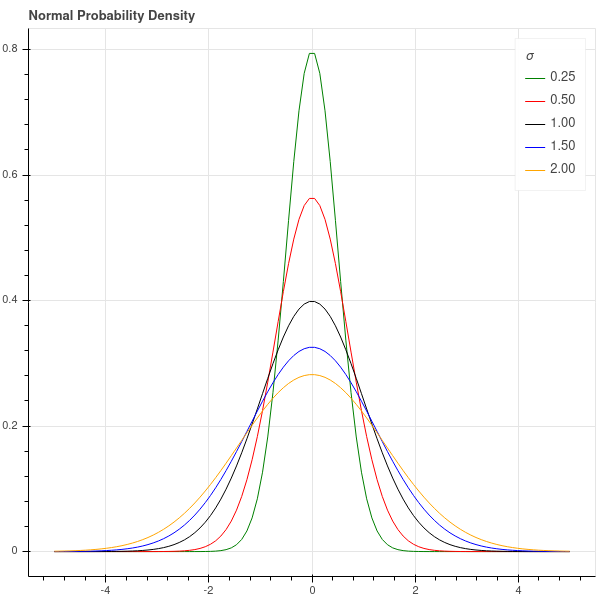
\includegraphics{chapters/img/density.png}

}

\caption{\label{fig-density}Normal Density}

\end{figure}

\hypertarget{conditional-probability-and-bayes-theorem}{%
\section{Conditional Probability and Bayes
Theorem}\label{conditional-probability-and-bayes-theorem}}

The theory of conditional probability gives a way to study how partial
information about an event informs us about the event as a whole. For
example, suppose you draw a card at random from a deck. As we've seen
earlier, the chance that card is an ace is \(1/13\). Now suppose that
you learn that (somehow) that the card is definitely not a jack, king,
or queen. Since there are 12 cards in the deck that are jacks, kings, or
queens, the card you've drawn is one of the remaining 40 cards, which
includes 4 aces. Thus the chance you are holding an ace is now
\(4/40=1/10\).

In terms of notation, if \(A\) is the event ``my card is an ace'' and
\(B\) is the event ``my card is not a jack, queen, or king'' then we say
that \emph{the probability of \(A\) given \(B\)} is \(1/10\). The
notation for this is \[
P(A|B) = 1/10.
\]

More generally, if \(A\) and \(B\) are events from a sample space \(X\),
and \(P(B)>0\), then \[
P(A|B) = \frac{P(A\cap B)}{P(B)},
\] so that \(P(A|B)\) measures the chance that \(A\) occurs among those
situations in which \(B\) occurs.

\hypertarget{bayes-theorem}{%
\subsection{Bayes Theorem}\label{bayes-theorem}}

Bayes theorem is a foundational result in probability.

\textbf{Theorem:} Bayes Theorem says \[
P(A|B) = \frac{P(B|A)P(A)}{P(B)}.
\]

If we use the definition of conditional probability given above, this is
straightforward: \[
\frac{P(B|A)P(A)}{P(B)} = \frac{P(B\cap A)}{P(B)} = P(A|B).
\]

\hypertarget{an-example}{%
\subsection{An example}\label{an-example}}

To illustrate conditional probability, let's consider what happens when
we administer the most reliable COVID-19 test, the PCR test, to an
individual drawn from the population at large. There are two possible
test results (positive and negative) and two possible true states of the
person being tested (infected and not infected). Suppose I go to the
doctor and get a COVID test which comes back positive. What is the
probability that I actually have COVID?

Let's let \(S\) and \(W\) stand for infected (sick) and not infected
(well), and let \(+/-\) stand for test positive or negative. Note that
there are four possible outcomes of our experiment:

\begin{itemize}
\tightlist
\item
  test positive and infected (S+) -- this is a \emph{true positive}.
\item
  test positive and not infected (W+) -- this is a \emph{false
  positive}.
\item
  test negative and infected (S-) -- this is a \emph{false negative}.
\item
  test negative and not infected (W-) -- this is a \emph{true negative}.
\end{itemize}

The
\href{https://www.icd10monitor.com/false-positives-in-pcr-tests-for-covid-19}{CDC
says} that the chance of a false positive -- that is, the percentage of
samples from well people that incorrectly yields a positive result -- is
about one-half of one percent, or 5 in 1000.

In other words, \[
P(+|W) = P(W+)/P(W) = 5/1000=1/200
\]

On the other hand, the CDC tells us that chance of a false negative is 1
in 4, so \[
P(-|S) = P(S-)/P(S) = .25.
\] Since \(P(S-)+P(S+)=P(S).\) since every test is either positive or
negative, we have \[
P(+|S) = .75.
\]

Suppose furthermore that the overall incidence of COVID-19 in the
population is p.~In other words, \(P(S)=p\) so \(P(W)=1-p\). Then
\[P(S+)=P(S)P(+|S)=.75p\] and \[
P(W+)=P(W)P(+|W)=.005(1-p).
\] Putting these together we get \(P(+)=.005+.745p\)

What I'm interested in is \(P(S|+)\) -- the chance that I'm sick, given
that my test result was positive. By Bayes Theorem, \[
P(S|+)=\frac{P(+|S)P(S)}{P(+)}=.75p/(.005+.745p)=\frac{750p}{5+745p}.
\]

As Figure~\ref{fig-covidfn} shows, if the population incidence is low
then a positive test is far from conclusive. Indeed, if the overall
incidence of COVID is one percent, then a positive test result only
implies a 60 percent chance that I am in fact infected.

Just to fill out the picture, we have \[
P(-) = P(S-)+P(W-)=(P(S)-P(S+))+(P(W)-P(W+))
\] which yields \[
P(-)=1-.005+.005p-.75p = .995-.745p.
\] Using Bayes Theorem, we obtain \[
P(S|-) = \frac{P(-|S)P(S)}{P(-)} = .25p/(.995-.745p) =\frac{250p}{995-745p}.
\] In this case, even though the false negative rate is pretty high (25
percent) overall, if the population incidence is one percent, then the
probability that you're sick given a negative result is only about
\(.25\) percent. So negative results are very likely correct!

\begin{figure}

{\centering 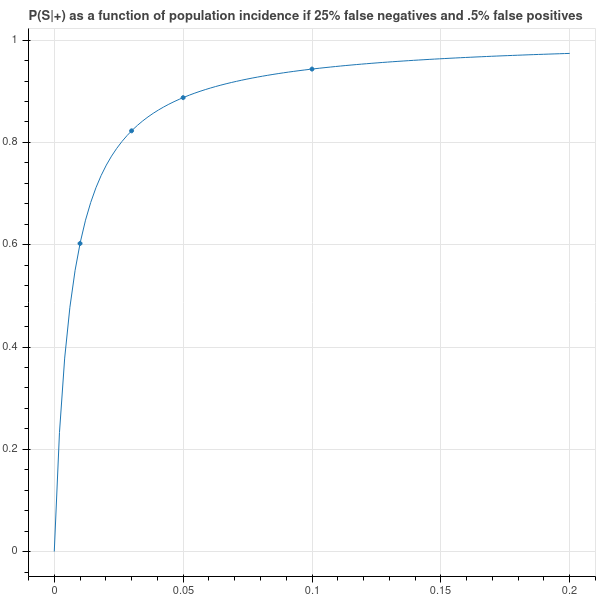
\includegraphics{chapters/img/covidfn.png}

}

\caption{\label{fig-covidfn}P(S\textbar+) vs P(S)}

\end{figure}

\hypertarget{independence}{%
\section{Independence}\label{independence}}

Independence is one of the fundamental concepts in probability theory.
Conceptually, two events are independent if the occurrence of one has
does not influence the likelihood of the occurrence of the other. For
example, successive flips of a coin are independent events, since the
result of the second flip doesn't have anything to do with the result of
the first. On the other hand, whether or not it rains today and tomorrow
are not independent events, since the weather tomorrow depends (in a
complicated way) on the weather today.

We can formalize this idea of independence using the following
definition.

\textbf{Definition:} Let \(X\) be a sample space and let \(A\) and \(B\)
be two events. Then \(A\) and \(B\) are \emph{independent} if
\(P(A\cap B)=P(A)P(B)\). Equivalently, \(A\) and \(B\) are independent
if \(P(A|B)=P(A)\) and \(P(B|A)=P(B)\).

\hypertarget{examples}{%
\subsection{Examples}\label{examples}}

\hypertarget{coin-flipping}{%
\subsubsection{Coin Flipping}\label{coin-flipping}}

Suppose our coin has a probability of heads given by a real number \(p\)
between \(0\) and \(1\), and we flip our coin \(N\) times. What is the
chance of gettting \(k\) heads, where \(0\le k\le N\)? Any particular
sequence of heads and tails containing \(k\) heads and \(N-k\) tails has
probability \[
P(\hbox{a particular sequence of $k$ heads among $N$ flips}) = p^{k}(1-p)^{N-k}.
\] In addition, there are \(\binom{N}{k}\) sequences of heads and tails
containing \(k\) heads. Thus the probability \(P(k,N)\) of \(k\) heads
among \(N\) flips is
\begin{equation}\protect\hypertarget{eq-binomial}{}{
P(k,N) = \binom{N}{k}p^{k}(1-p)^{N-k}.
}\label{eq-binomial}\end{equation}

Notice that the binomial theorem gives us \(\sum_{k=0}^{N} P(k,N) =1\)
which is a reassuring check on our work.

The probability distribution on the set \(X=\{0,1,\ldots,N\}\) given by
\(P(k,N)\) is called the \emph{binomial distribution} with parameters
\(N\) and \(p\).

\hypertarget{a-simple-mixture}{%
\subsubsection{A simple `mixture'}\label{a-simple-mixture}}

Now let's look at an example of events that are not independent. Suppose
that we have two coins, with probabilities of heads \(p_1\) and \(p_2\)
respectively; and assume these probabilities are different. We play the
a game in which we first choose one of the two coins (with equal chance)
and then flip it twice. Is the result of the second flip independent of
the first? In other words, is \(P(HH)=P(H)^2\)?

This type of situation is called a `mixture distribution' because the
probability of a head is a ``mixture'' of the probability coming from
the two different coins.

The chance that the first flip is a head is \((p_1+p_2)/2\) because it's
the chance of picking the first coin, and then getting a head, plus the
chance of picking the second, and then getting a head. The chance of
getting two heads in a row is \((p_1^2+p_2^2)/2\) because it's the
chance, having picked the first coin, of getting two heads, plus the
chance, having picked the second, of getting two heads.

Since \[
\frac{p_1^2+p_2^2}{2}\not=\left(\frac{p_1+p_2}{2}\right)^2
\] we see these events are not independent.

In terms of conditional probabilities, the chance that the second flip
is a head, given that the first flip is, is computed as: \[
P(HH|H) = \frac{p_1^2+p_2^2}{p_1+p_2}.
\] From the Cauchy-Schwartz inequality one can show that \[
\frac{p_1^2+p_2^2}{p_1+p_2}>\frac{p_1+p_2}{2}.
\]

Why should this be? Why should the chance of getting a head on the
second flip go up given that the first flip was a head? One way to think
of this is that the first coin flip contains a little bit of information
about which coin we chose. If, for example \(p_1>p_2\), and our first
flip is heads, then it's just a bit more likely that we chose the first
coin. As a result, the chance of getting another head is just a bit more
likely than if we didn't have that information. We can make this precise
by considering the conditional probability \(P(p=p_1|H)\) that we've
chosen the first coin given that we flipped a head. From Bayes' theorem:

\[
P(p=p_1|H) = \frac{P(H|p=p_1)P(p=p_1)}{P(H)}=\frac{p_1}{p_1+p_2}=\frac{1}{1+(p_2/p_1)}>\frac{1}{2}
\] since \((1+(p_2/p_1))<2\).

\textbf{Exercise:} Push this argument a bit further. Let
\(p_1=\max(p_1,p_2)\) Let \(P_N\) be the conditional probability of
getting heads assuming that the first \(N\) flips were heads. Show that
\(P_N\to p_1\) as \(N\to\infty\). All those heads piling up make it more
and more likely that you're flipping the first coin and so the chance of
getting heads approaches \(p_1\).

\hypertarget{an-example-with-a-continuous-distribution}{%
\subsubsection{An example with a continuous
distribution}\label{an-example-with-a-continuous-distribution}}

Suppose that we return to our example of a thermometer which measures
the ambient temperature with an error that is distributed according to
the normal distribution, as in Equation~\ref{eq-normal}. Suppose that we
make 10 independent measurements \(t_1,\ldots, t_{10}\) of the true
temperature \(t_0\). What can we say about the distribution of these
measurements?

In this case, independence means that \[
P=P(|t_1-t_0|<\delta,|t_2-t_0|<\delta,\ldots) = P(|t_1-t_0|<\delta)P(|t_2-t_0|<\delta)\cdots P(|t_{10}-t_{0}|<\delta)
\] and therefore \[
P = \left(\frac{1}{\sigma\sqrt{2\pi}}\right)^{10}\int_{-\delta}^{\delta}\cdots\int_{-\delta}^{\delta}
e^{-(\sum_{i=1}^{10} x_i^2)/2\sigma^2} dx_1\cdots dx_{10}
\]

One way to look at this is that the vector \(\mathbf{e}\) of errors
\((|t_1-t_0|,\ldots,|t_{10}-t_0|)\) is distributed according to a
\emph{multivariate gaussian distribution}:
\begin{equation}\protect\hypertarget{eq-multivariategaussian}{}{
P(\mathbf{e}\in U) =\left(\frac{1}{\sigma\sqrt{2\pi}}\right)^{10}\int_{U}
e^{-\|x\|^2/2\sigma^2} d\mathbf{x}
}\label{eq-multivariategaussian}\end{equation}

where \(U\) is a region in \(\mathbf{R}^{10}\).

The multivariate gaussian can also describe situations where
independence does not hold. For simplicity, let's work in two dimensions
and consider the probability density on \(\mathbf{R}^{2}\) given by \[
P(\mathbf{e}\in U) = A\int_{U} e^{-(x_1^2-x_1x_2+x_2^2)/2\sigma^2} d\mathbf{x}.
\] where the constant \(A\) is chosen so that \[
A\int_{\mathbf{R}^{2}}e^{-(x_1^2-x_1x_2+x_2^2)/2\sigma^2}d\mathbf{x} = 1.
\]

This density function as a ``bump'' concentrated near the origin in
\(\mathbf{R}^{2}\), and its level curves are a family of ellipses
centered at the origin. See Figure~\ref{fig-multivariate} for a plot of
this function with \(\sigma=1\).

\begin{figure}

{\centering 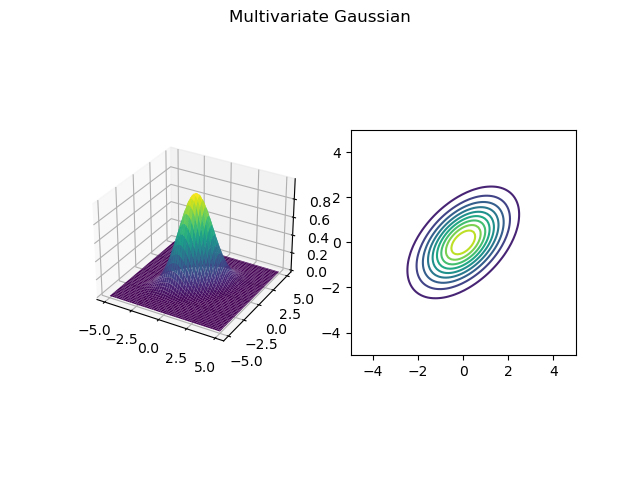
\includegraphics{chapters/img/ellipse.png}

}

\caption{\label{fig-multivariate}Multivariate Gaussian}

\end{figure}

In this situation we can look at the conditional probability of the
first variable given the second, and see that the two variables are not
independent. Indeed, if we fix \(x_2\), then the distribution of \(x_1\)
depends on our choice of \(x_2\). We could see this by a calculation, or
we can just look at the graph: if \(x_2=0\), then the most likely values
of \(x_1\) cluster near zero, while if \(x_2=1\), then the most likely
values of \(x_1\) cluster somewhere above zero.

\hypertarget{random-variables-mean-and-variance}{%
\section{Random Variables, Mean, and
Variance}\label{random-variables-mean-and-variance}}

Typically, when we are studying a random process, we aren't necessarily
accessing the underlying events, but rather we are making measurements
that provide us with some information about the underlying events. For
example, suppose our sample space \(X\) is the set of throws of a pair
of dice, so \(X\) contains the \(36\) possible combinations that can
arise from the throws. What we are actually interested is the sum of the
values of the two dice -- that's our ``measurement'' of this system.
This rather vague notion of a measurement of a random system is captured
by the very general idea of a \emph{random variable}.

\textbf{Definition:} Let \(X\) be a sample space with probability
function \(P\). A \emph{random variable} on \(X\) is a function
\(f:X\to \mathbb{R}\).

Given a random variable \(f\), we can use the probability measure to
decide how likely \(f\) is to take a particular value, or values in a
particular set by the formula \[
P(f(x)\in U) = P(f^{-1}(U))
\]

In the dice rolling example, the random variable \(S\) that assigns
their sum to the pair of values obtained on two dice is a random
variable. Those values lie between \(2\) and \(12\) and we have \[
P(S=k) = P(S^{-1}(\{k\}))=P(\{(x,y): x+y=k\})
\] where \((x,y)\) runs through \(\{1,2,\ldots,6\}^{2}\) representing
the two values and \(P((x,y))=1/36\) since all throws are equally
likely.

Let's look at a few more examples, starting with what is probably the
most fundamental of all.

\textbf{Definition:} Let \(X\) be a sample space with two elements, say
\(H\) and \(T\), and suppose that \(P(H)=p\) for some \(0\le p\le 1\).
Then the random variable that satisfies \(f(H)=1\) and \(f(T)=0\) is
called a Bernoulli random variable with parameter \(p\).

In other words, a Bernoulli random variable gives the value \(1\) when a
coin flip is heads, and \(0\) for tails.

Now let's look at what we earlier called the binomial distribution.

\textbf{Definition:} Let \(X\) be a sample space consisting of strings
of \(H\) and \(T\) of length \(N\), with the probability of a
\emph{particular string} \(S\) with \(k\) heads and \(N-k\) tails given
by \[
P(S)=p^{k}(1-p)^{N-k}
\] for some \(0\le p\le 1\). In other words, \(X\) is the sample space
consisting of \(N\) independent flips of a coin with probability of
heads given by \(p\).

Let \(f:X\to \mathbb{R}\) be the function which counts the number of
\(H\) in the string. We can express \(f\) in terms of Bernoulli random
variables; indeed, \[
f=X_1+\ldots+X_N
\] where each \(X_i\) is a Bernoulli random variable with parameter
\(p\).

Now \[
P(f=k) = \binom{N}{k}p^{k}(1-p)^{N-k}
\] since \(f^{-1}(\{k\})\) is the number of elements in the subset of
strings of \(H\) and \(T\) of length \(N\) containing exactly \(k\)
\(H\)'s. This is our old friend the binomial distribution. So \emph{a
binomial distribution is the distribution of the sum of \(N\)
independent Bernoulli random variables.}

For an example with a continuous random variable, suppose our sample
space is \(\mathbf{R}^{2}\) and the probability density is the simple
multivariate normal \[
P(\mathbf{x}\in U) = \left(\frac{1}{\sqrt{2\pi}}\right)^2\int_{U} e^{-\|\mathbf{x}\|^2/2} d\mathbf{x}.
\] Let \(f\) be the random variable \(f(\mathbf{x})=\|\mathbf{x}\|\).
The function \(f\) measures the Euclidean distance of a randomly drawn
point from the origin. The set
\[U=f^{-1}([0,r))\subseteq\mathbf{R}^{2}\] is the circle of radius \(r\)
in \(\mathbf{R}^{2}\). The probability that a randomly drawn point lies
in this circle is \[
P(f<r) = \left(\frac{1}{\sqrt{2\pi}}\right)^2\int_{U} e^{-\|\mathbf{x}\|^2/2} d\mathbf{x}.
\]

We can actually evaluate this integral in closed form by using polar
coordinates. We obtain \[
P(f<r) = \left(\frac{1}{\sqrt{2\pi}}\right)^2\int_{\theta=0}^{2\pi}\int_{\rho=0}^{r} e^{-\rho^2/2}\rho d\rho d\theta.
\] Since \[
\frac{d}{d\rho}e^{-\rho^2/2}=-\rho e^{-\rho^2/2}
\] we have \begin{align*}
P(f<r)&=-\frac{1}{2\pi}\theta e^{-\rho^2/2}|_{\theta=0}^{2\pi}|_{\rho=0}^{r}\cr
&=1-e^{-r^2/2}\cr
\end{align*}

The probability density associated with this random variable is the
derivative of \(1-e^{-r^2/2}\) \[
P(f\in [a,b])=\int_{r=a}^{b} re^{-r^2/2} dr
\] as you can see by the fundamental theorem of calculus. This density
is drawn in Figure~\ref{fig-maxwell} where you can see that the points
are clustered at a distance of \(1\) from the origin.

\begin{figure}

{\centering 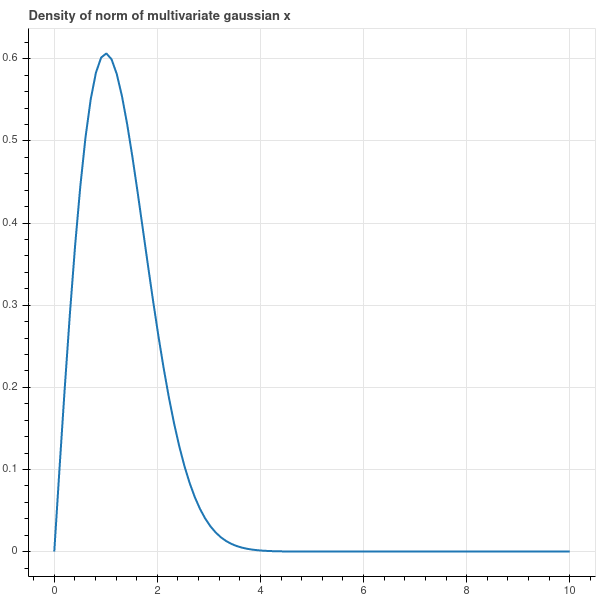
\includegraphics{chapters/img/maxwell.png}

}

\caption{\label{fig-maxwell}Density of the Norm}

\end{figure}

\hypertarget{independence-and-random-variables}{%
\subsection{Independence and Random
Variables}\label{independence-and-random-variables}}

We can extend the notion of independence from events to random
variables.

\textbf{Definition:} Let \(f\) and \(g\) be two random variables on a
sample space \(X\) with probability \(P\). Then \(f\) and \(g\) are
independent if, for all intervals \(U\) and \(V\) in \(\mathbb{R}\), the
events \(f^{-1}(U)\) and \(g^{-1}(V)\) are independent.

For discrete probability distributions, this means that, for all
\(a,b\in\mathbb{R}\), \[
P(f=a\hbox{\ and\ }g=b)=P(f=a)P(g=b).
\]

For continous probability distributions given by a density function
\(P(x)\), independence can be more complicated to figure out.

\hypertarget{expectation-mean-and-variance}{%
\subsection{Expectation, Mean and
Variance}\label{expectation-mean-and-variance}}

The most fundamental tool in the study of random variables is the
concept of ``expectation'', which is a fancy version of average. The
word ``mean'' is a synonym for expectation -- the mean of a random
variable is the same as its expectation or ``expected value.''

\textbf{Definition:} Let \(X\) be a sample space with probability
measure \(P\). Let \(f:X\to \mathbb{R}\) be a random variable. Then the
\emph{expectation} or \emph{expected value} \(E[f]\) of \(f\) is \[
E[f] = \int_X f(x)dP.
\] More specifically, if \(X\) is discrete, then \[
E[f] = \sum_{x\in X} f(x)P(x)
\] while if \(X\) is continuous with probability density function
\(p(x)dx\) then \[
E[f] = \int_{X} f(x)p(x)dx.
\]

If \(f\) is a Bernoulli random variable with parameter \(p\), then \[
E[f] = 1\cdot p+0\cdot (1-p) = p
\]

If \(f\) is a binomial random variable with parameters \(p\) and \(N\),
then \[
E[f] = \sum_{i=0}^{N} i\binom{N}{i}p^{i}(1-p)^{N-i}
\] One can evaluate this using some combinatorial tricks, but it's
easier to apply this basic fact about expectations.

\textbf{Proposition:} Expectation is linear: \(E[aX+bY]=aE[X]+bE[Y]\)
for random variables \(X,Y\) and constants \(a\) and \(b\).

The proof is an easy consequence of the expression of \(E\) as a sum (or
integral).

Since a binomial random variable \(Z\) with parameters \(N\) and \(p\)
is the sum of \(N\) Bernoulli random variables, its expectation is \[
E[X_1+\cdots+X_N]=Np.
\]

A more sophisticated property of expectation is that it is
multiplicative when the random variables are independent.

\textbf{Proposition:} Let \(f\) and \(g\) be two independent random
variables. Then \(E[fg]=E[f]E[g]\).

\textbf{Proof:} Let's suppose that the sample space \(X\) is discrete.
By definition, \[
E[f]=\sum_{x\in X}f(x)P(x)
\] and we can rewrite this as \[
E[f]=\sum_{a\in\mathbf{R}} aP(\{x: f(x)=a\}).
\] Let \(Z\subset\mathbb{R}\) be the range of \(f\). Then \begin{align*}
E[fg]&=\sum_{a\in Z} aP(\{x: fg(x)=a\}) \\
&=\sum_{a\in Z}\sum_{(u,v)\in\genfrac{}{}{0pt}{}{\mathbf{Z}^{2}}{uv=a}}aP(\{x:f(x)=u\hbox{\ and\ }g(x)=v\}) \\
&=\sum_{a\in Z}\sum_{\genfrac{}{}{0pt}{}{\mathbf{Z}^{2}}{uv=a}}uvP(\{x:f(x)=u\})P(\{x:g(x)=v\}) \\
&=\sum_{u\in Z}uP(\{x:f(x)=u\})\sum_{v\in Z}vP(\{x:f(x)=v\}) \\
&=E[f]E[g]
\end{align*}

\hypertarget{variance-1}{%
\subsubsection{Variance}\label{variance-1}}

The variance of a random variable is a measure of its dispersion around
its mean.

\textbf{Definition:} Let \(f\) be a random variable. Then the variance
is the expression \[
\sigma^2(f) = E[(f-E[f])^2]=E[f^2]-(E[f])^2
\] The square root of the variance is called the ``standard deviation.''

The two formulae for the variance arise from the calculation \[
E[(f-E[f])^2]=E[(f^2-2fE[f]+E[f]^2)]=E[f^2]-2E[f]^2+E[f]^2=E[f^2]-E[f]^2.
\]

To compute the variance of the Bernoulli random variable \(f\) with
parameter \(p\), we first compute \[
E[f^2]=p(1)^2+(1-p)0^2=p.
\] Since \(E[f]=p\), we have \[
\sigma^2(f)=p-p^2=p(1-p).
\]

If \(f\) is the binomial random variable with parameters \(N\) and
\(p\), we can again use the fact that \(f\) is the sum of \(N\)
Bernoulli random variables \(X_1+\cdots+X_n\) and compute

\begin{align*}
E[(\sum_{i}X_i)^2]-E[\sum_{i} X_{i}]^2 &=E[\sum_{i} X_i^2+\sum_{i,j}X_{i}X_{j}]-N^2p^2\\
&=Np+N(N-1)p^2-N^2p^2 \\
&=Np(1-p)
\end{align*}

where we have used the fact that the square \(X^2\) of a Bernoulli
random variable is equal to \(X\).

For a continuous example, suppose that we consider a sample space
\(\mathbb{R}\) with the normal probability density \[
P(x) = \frac{1}{\sigma\sqrt{2\pi}}e^{-x^2/2\sigma^2}dx.
\]

The mean of the random variable \(x\) is \[
E[x] =\frac{1}{\sigma\sqrt{2\pi}}\int_{-\infty}^{\infty} xe^{-x^2/2\sigma^2}dx=0
\]

since the function being integrated is odd. The variance is

\[
E[x^2] = \frac{1}{\sigma\sqrt{2\pi}}\int_{-\infty}^{\infty} x^2e^{-x^2/2\sigma^2}dx.
\]

The trick to evaluating this integral is to consider the derivative:

\[
\frac{d}{d\sigma}\left[\frac{1}{\sigma\sqrt{2\pi}}\int_{-\infty}^{\infty}e^{-x^2/(2\sigma^2)}dx\right]=0
\]

where the result is zero since the quantity being differentiated is a
constant (namely \(1\)). Sorting through the resulting equation leads to
the fact that

\[
E[x^2]=\sigma^2
\]

so that the \(\sigma^2\) parameter in the normal distribution really
\emph{is} the variance of the associated random variable.

\hypertarget{models-and-likelihood}{%
\section{Models and Likelihood}\label{models-and-likelihood}}

A \emph{statistical model} is a mathematical model that accounts for
data via a process that incorporates random behavior in a structured
way. We have seen several examples of such models in our discussion so
far. For example, the Bernoulli process that describes the outcome of a
series of coin flips as independent choices of heads or tails with
probability \(p\) is a simple statistical model; our more complicated
mixture model in which we choose one of two coins at random and then
flip that is a more complicated model.\\
Our description of the variation in temperature measurements as arising
from perturbations from the true temperature by a normally distributed
amount is another example of a statistical model, this one involving a
continuous random variable.

When we apply a mathematical model to understand data, we often have a
variety of parameters in the model that we must adjust to get the model
to best ``fit'' the observed data. For example, suppose that we observe
the vibrations of a block attached to a spring. We know that the motion
is governed by a second order linear differential equation, but the
dynamics depend on the mass of the block, the spring constant, and the
damping coefficient. By measuring the dynamics of the block over time,
we can try to work backwards to figure out these parameters, after which
we will be able to predict the block's motion into the future.

\hypertarget{sec-mlcoin}{%
\subsection{Maximum Likelihood (Discrete Case)}\label{sec-mlcoin}}

To see this process in a statistical setting, let's return to the simple
example of a coin flip. The only parameter in our model is the
probability \(p\) of getting heads on a particular flip. Suppose that we
flip the coin \(100\) times and get \(55\) heads and \(45\) tails. What
can we say about \(p\)?

We will approach this question via the ``likelihood'' function for our
data. We ask: for a particular value of the parameter \(p\), how likely
is this outcome? From Equation~\ref{eq-binomial} we have \[
P(55H,45T)=\binom{100}{55}p^{55}(1-p)^{45}.
\]

This function is plotted in Figure~\ref{fig-beta}. As you can see from
that plot, it is extremely unlikely that we would have gotten \(55\)
heads if \(p\) was smaller than \(.4\) or greater than \(.7\), while the
\emph{most likely} value of \(p\) occurs at the maximum value of this
function, and a little calculus tells us that this point is where
\(p=.55\). This \emph{most likely} value of \(p\) is called the
\emph{maximum likelihood estimate} for the parameter \(p\).

\begin{figure}

{\centering 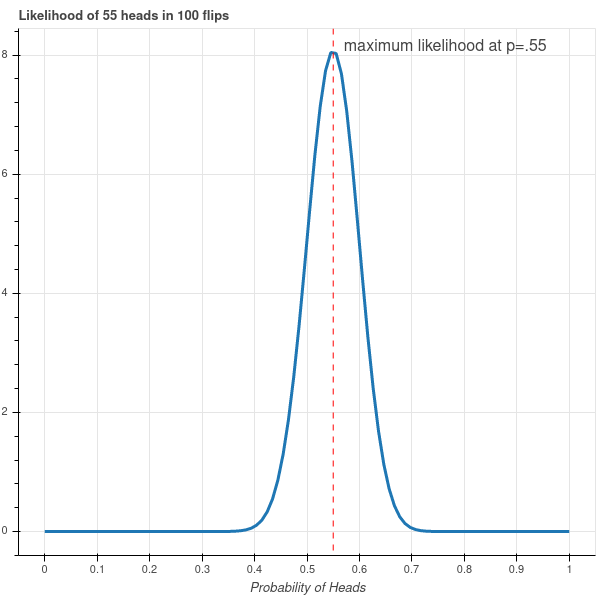
\includegraphics{chapters/img/beta.png}

}

\caption{\label{fig-beta}Likelihood Plot}

\end{figure}

\hypertarget{maximum-likelihood-continuous-case}{%
\subsection{Maximum Likelihood (Continuous
Case)}\label{maximum-likelihood-continuous-case}}

Now let's look at our temperature measurements where the error is
normally distributed with variance parameter \(\sigma^2\). As we have
seen earlier, the probability density of errors
\(\mathbf{x}=(x_1,\ldots,x_n)\) of \(n\) independent measurements is \[
P(\mathbf{x}) = \left(\frac{1}{\sigma\sqrt{2\pi}}\right)^{n}e^{-\|\mathbf{x}\|^2/(2\sigma^2)}d\mathbf{x}.
\] (see Equation~\ref{eq-multivariategaussian}). What should we use as
the parameter \(\sigma\)? We can ask which choice of \(\sigma\) makes
our data \emph{most likely}. To calculate this, we think of the
probability of a function of \(\sigma\) and use Calculus to find the
maximum. It's easier to do this with the logarithm.

\[
\log P(\mathbf{x})=\frac{-\|\mathbf{x}\|^2}{2\sigma^2}-n\log{\sigma}+C
\] where \(C\) is a constant that we'll ignore. Taking the derivative
and setting it to zero, we obtain \[
-\|\mathbf{x}\|^2\sigma^{-3}-n\sigma^{-1}=0
\] which gives the formula \[
\sigma^2=\frac{\|\mathbf{x}\|^2}{n}
\]

This should look familiar! The maximum likelihood estimate of the
variance is the \emph{mean-squared-error}.

\hypertarget{sec-LRLike}{%
\subsection{Linear Regression and likelihood}\label{sec-LRLike}}

In our earlier lectures we discussed linear regression at length. Our
introduction of ideas from probability give us new insight into this
fundamental tool. Consider a statistical model in which certain measured
values \(y\) depend linearly on \(x\) up to a normally distributed
error: \[
y=mx+b+\epsilon
\] where \(\epsilon\) is drawn from the normal distribution with
variance \(\sigma^2\).

The classic regression setting has us measuring a collection of \(N\)
points \((x_i,y_i)\) and then asking for the ``best'' \(m\), \(b\), and
\(\sigma^2\) to explain these measurements. Using the likelihood
perspective, each value \(y_i-mx_i-b\) is an independent draw from the
normal distribution with variance \(\sigma^2\), exactly like our
temperature measurements in the one variable case.

The likelihood (density) of those draws is therefore \[
P = \left(\frac{1}{\sigma\sqrt{2\pi}}\right)^Ne^{-\sum_{i}(y_i-mx_i-b)^2/(2\sigma^2)}.
\] What is the maximum likelihood estimate of the parameters \(m\),
\(b\), and \(\sigma^2\)?

To find this we look at the logarithm of \(P\) and take derivatives. \[
\log(P) = -N\log(\sigma) -\frac{1}{2\sigma^2}\sum_{i}(y_i-mx_i-b)^2.
\]

As far as \(m\) and \(b\) are concerned, the minimum comes from the
derivatives with respect to \(m\) and \(b\) of \[
\sum_{i}(y_i-mx_i-b)^2.
\] In other words, the maximum likelihood estimate \(m_*\) and \(b_*\)
for \(m\) and \(b\) are \emph{exactly the ordinary least squares
estimates.}

As far as \(\sigma^2\) is concerned, we find just as above that the
maximum likelihood estimate \(\sigma^2_*\) is the mean squared error \[
\sigma^2_*=\frac{1}{N}\sum_{i}(y_i-m_*x_i-b_*)^2.
\]

The multivariate case of regression proposes a model of the form \[
Y=X\beta+\epsilon
\] and a similar calculation again shows that the least squares
estimates for \(\beta\) are the maximum likelihood values for this
model.

\hypertarget{bayesian-inference}{%
\section{Bayesian Inference}\label{bayesian-inference}}

We conclude our review of ideas from probability by examining the
Bayesian perspective on data.

Suppose that we wish to conduct an experiment to determine the
temperature outside our house. We begin our experiment with a
statistical model that is supposed to explain the variability in the
results. The model depends on some parameters that we wish to estimate.
For example, the parameters of our experiment might be the `true'
temperature \(t_*\) and the variance \(\sigma^2\) of the error.

From the Bayesian point of view, at the beginning of this experiment we
have an initial sense of what the temperature is likely to be, expressed
in the form of a probability distribution. This initial information is
called the \emph{prior} distribution.

For example, if we know that it's December in Connecticut, our prior
distribution might say that the temperature is more likely to be between
20 and 40 degrees Fahrenheit and is quite unlikely to be higher than 60
or lower than 0. So our prior distribution might look like
Figure~\ref{fig-tempprior}.

\begin{figure}

{\centering 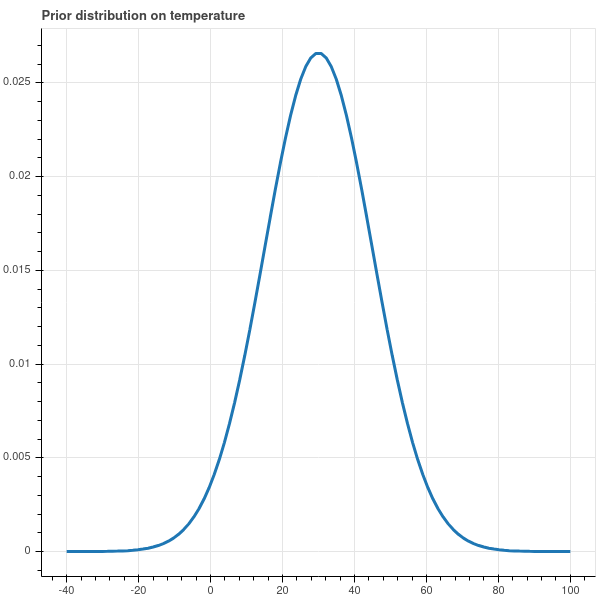
\includegraphics{chapters/img/prior.png}

}

\caption{\label{fig-tempprior}Prior Distribution on Temperature}

\end{figure}

If we really have no opinion about the temperature other than its
between say, \(-20\) and \(100\) degrees, our prior distribution might
be uniform over that range, as in Figure~\ref{fig-uniformprior}.

\begin{figure}

{\centering 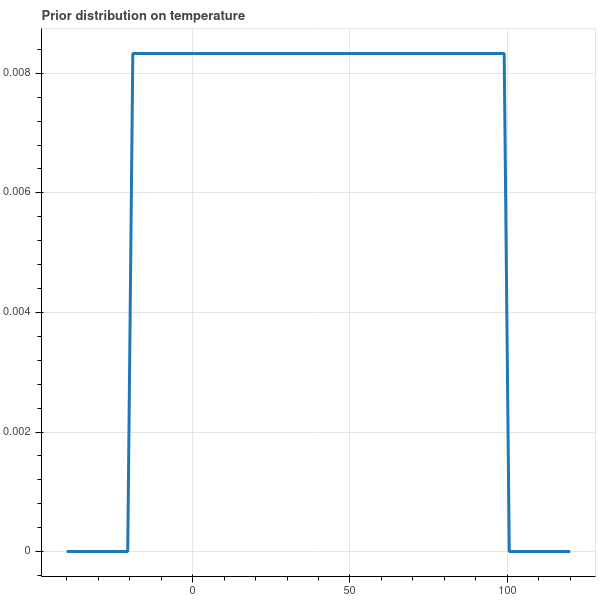
\includegraphics{chapters/img/uniform.png}

}

\caption{\label{fig-uniformprior}Uniform Prior}

\end{figure}

The choice of a prior will guide the interpretation of our experiments
in ways that we will see shortly.

The next step in our experiment is the collection of data. Suppose we
let \(\mathbf{t}=(t_1,t_2,\ldots, t_n)\) be a random variable
representing \(n\) independent measurements of the temperature. We
consider the \emph{joint distribution} of the parameters \(t_*\) and
\(\sigma^2\) and the possible measurements \(\mathbf{t}\): \[
P(\mathbf{t},t_*,\sigma^2)=\left(\frac{1}{\sigma\sqrt{2\pi}}\right)^{n}e^{-\|\mathbf{t}-t_*\mathbf{e}\|^2/(2\sigma^2)}
\] where \(\mathbf{e}=(1,1,\ldots, 1)\).

The conditional probability \(P(t_{*},\sigma^2|\mathbf{t})\) is the
distribution of the values of \(t_*\) and \(\sigma^2\)\emph{given}a
value of the \(\mathbf{t}\). This is what we hope to learn by our
experiment -- namely, if we make a particular measurement, what does it
tell us about \(t_*\) and \(\sigma^2\)?

Now suppose that we actually make some measurements, and so we obtain a
specific set of values \(\mathbf{t}_0\) for \(\mathbf{t}\).

By Bayes Theorem, \[
P(t_{*},\sigma^2|\mathbf{t}=\mathbf{t}_0) = \frac{P(\mathbf{t}=\mathbf{t}_0|t_{*},\sigma^2)P(t_{*},\sigma^2)}{P(\mathbf{t}=\mathbf{t}_0)}
\] We interpret this as follows:

\begin{itemize}
\tightlist
\item
  the left hand side \(P(t_{*},\sigma^2|\mathbf{t}=\mathbf{t}_0)\) is
  called the \emph{posterior distribution} and is the distribution of
  \(t_{*}\) and \(\sigma^2\) obtained by \emph{updating our prior
  knowledge with the results of our experiment.}
\item
  The probability \(P(\mathbf{t}=\mathbf{t}_{0}|t_{*},\sigma^2)\) is the
  probability of obtaining the measurements we found for a particular
  value of the parameters \(t_{*}\) and \(\sigma^2\).
\item
  The probability \(P(t_{*},\sigma^2)\) is the \emph{prior distribution}
  on the parameters that reflects our initial impression of the
  distribution of these parameters.
\item
  The denominator \(P(\mathbf{t}=\mathbf{t}_{0})\) is the total
  probability of the results that we obtained, and is the integral over
  the distribution of the parameters weighted by their prior
  probability: \[
  P(\mathbf{t}=\mathbf{t}_{0})=\int_{t_{*},\sigma^2}P(\mathbf{t}=\mathbf{t}_{0}|t_{*},\sigma^2)P(t_{*},\sigma^2)
  \]
\end{itemize}

\hypertarget{bayesian-experiments-with-the-normal-distribution}{%
\subsection{Bayesian experiments with the normal
distribution}\label{bayesian-experiments-with-the-normal-distribution}}

To illustrate these Bayesian ideas, we'll consider the problem of
measuring the temperature, but for simplicity let's assume that we fix
the variance in our error measurements at \(1\) degree. Let's use the
prior distribution on the true temperature that I proposed in
Figure~\ref{fig-tempprior}, which is a normal distribution with variance
\(15\) ``shifted'' to be centered at \(30\): \[
P(t_*)=\left(\frac{1}{\sqrt{2\pi}}\right)e^{-(t_*-30)^2/30}.
\] The expected value \(E[t]\) -- the mean of the this distribution --
is \(30\).

Since the error in our measurements is normally distributed with
variance \(1\), we have \[
P(t-t_{*})=\left(\frac{1}{\sqrt{2\pi}}\right)e^{-(t-t_{*})^2/2}
\] or as a function of the absolute temperature, we have \[
P(t,t_{*}) = \left(\frac{1}{\sqrt{2\pi}}\right)e^{-(t-t_*)^2/2}.
\]

Now we make a bunch of measurements to obtain
\(\mathbf{t}_0=(t_1,\ldots, t_n)\). We have \[
P(\mathbf{t}=\mathbf{t}_0|t_{*}) = \left(\frac{1}{\sqrt{2\pi}}\right)^ne^{-\|\mathbf{t}-t_*\mathbf{e}\|^2/2}.
\]

The total probability \(T=P(\mathbf{t}=\mathbf{t_0})\) is hard to
calculate, so let's table that for a while. The posterior probability is
\[
P(t_{*}|\mathbf{t}=\mathbf{t}_{0}) = \frac{1}{T}
\left(\frac{1}{\sqrt{2\pi}}\right)^ne^{-\|\mathbf{t}-t_*\mathbf{e}\|^2/2}
\left(\frac{1}{\sqrt{2\pi}}\right)e^{-(t_*-30)^2/30}.
\]

Leaving aside the multiplicative constants for the moment, consider the
exponential \[
e^{-(\|\mathbf{t}-t_{*}\mathbf{e}\|^2/2+(t_{*}-30)^2)/30}.
\] Since \(\mathbf{t}\) is a vector of constants -- it is a vector of
our particular measurements -- the exponent \[
\|\mathbf{t}-t_{*}\mathbf{e}\|^2/2+(t_{*}-30)^2/30 = (t_{*}-30)^2/30+\sum_{i} (t_{i}-t_{*})^2/2
\] is a quadratic polynomial in \(t_{*}\) that simplifies: \[
(t_{*}-30)^2/30+\sum_{i} (t_{i}-t_{*})^2/2 = At_{*}^2+Bt_{*}+C.
\] Here \[
A=(\frac{1}{30}+\frac{n}{2}),
\] \[
B=-2-\sum_{i} t_{i}
\] \[
C=30+\frac{1}{2}\sum_{i} t_{i}^2.
\]

We can complete the square to write \[
At_{*}^2+Bt_{*}+C = (t_{*}-U)^2/2V +K
\] where \[
U=\frac{2+\sum_{i}t_{i}}{\frac{1}{15}+n}
\] and \[
V=\frac{1}{\frac{1}{15}+n}.
\] So up to constants that don't involve \(t_{*}\), the posterior
density is of the form \[
e^{(t_{*}-U)^2/2V}
\] and since it is a probability density, the constants must work out to
give total integral of \(1\). Therefore the posterior density is a
normal distribution centered at \(U\) and with variance \(V\). Here
\(U\) is called the\emph{posterior mean}and \(V\) the\emph{posterior
variance}.

To make this explicit, suppose \(n=5\) and we measured the following
temperatures: \[
40, 41,39, 37, 44
\] The mean of these observations is \(40.2\) and the variance is
\(5.4\).

A calculation shows that the posterior mean is \(40.1\) and the
posterior variance is \(0.2\). Comparing the prior with the posterior,
we obtain the plot in Figure~\ref{fig-comparison}. The posterior has a
sharp peak at \(40.1\) degrees. This value is just a bit smaller than
the mean of the observed temperatures which is \(40.2\) degrees. This
difference is caused by the prior -- our prior distribution said the
temperature was likely to be around \(30\) degrees, and so the prior
pulls the observed mean a bit towards the prior mean taking into account
past experience. Because the variance of the prior is large, it has a
relatively small influence on the posterior.

The general version of the calculation above is summarized in this
proposition.

\textbf{Proposition:} Suppose that our statistical model for an
experiment proposes that the measurements are normally distributed
around an (unknown) mean value of \(\mu\) with a (fixed) variance
\(\sigma^2\). Suppose further that our prior distribution on the unknown
mean \(\mu\) is normal with mean \(\mu_0\) and variance \(\tau^2\).
Suppose we make measurements \[
y_1,\ldots, y_n
\] with mean \(\overline{y}\). Then the posterior distribution of
\(\mu\) is again normal, with posterior variance \[
\tau'^2 = \frac{1}{\frac{1}{\tau^2}+\frac{n}{\sigma^2}}
\] and posterior mean \[
\mu' = \frac{\frac{\mu_0}{\tau^2}+\frac{n}{\sigma^2}\overline{y}}{\frac{1}{\frac{1}{\tau^2}+\frac{n}{\sigma^2}}}
\]

So the posterior mean is a sort of weighted average of the sample mean
and the prior mean; and as \(n\to\infty\), the posterior mean approaches
the sample mean -- in other words, as you get more data, the prior has
less and less influence on the results of the experiment.

\begin{figure}

{\centering 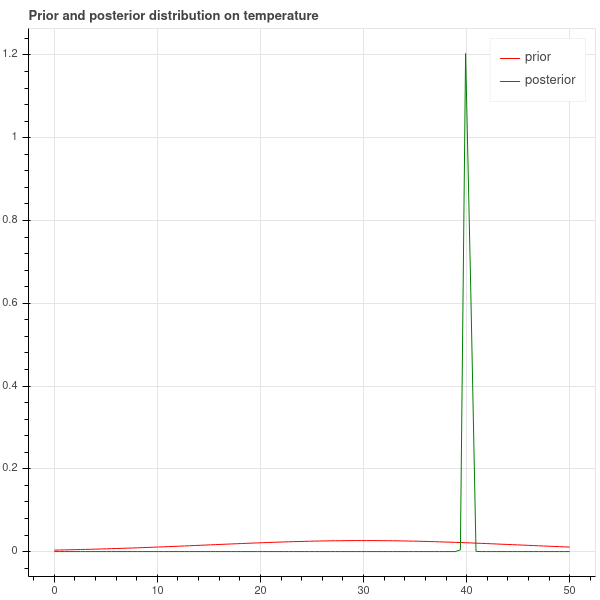
\includegraphics{chapters/img/priorposterior.png}

}

\caption{\label{fig-comparison}Prior and Posterior}

\end{figure}

\hypertarget{bayesian-coin-flipping}{%
\subsection{Bayesian coin flipping}\label{bayesian-coin-flipping}}

For our final example in this fast overview of ideas from probability,
we consider the problem of deciding whether a coin is fair. Our
experiment consists of \(N\) flips of a coin with unknown probability
\(p\) of heads, so the data consists of the number \(h\) of heads out of
the \(N\) flips. To apply Bayesian reasoning, we need a prior
distribution on \(p\). Let's first assume that we have no reason to
prefer one value of \(p\) over another, and so we choose for our prior
the uniform distribution on \(p\) between \(0\) and \(1\).

We wish to analyze \(P(p|h)\), the probability distribution of \(p\)
given \(h\) heads out of \(N\) flips. Bayes Theorem gives us: \[
P(p|h) = \frac{P(h|p)P(p)}{P(h)}
\] where \[
P(h|p) = \binom{N}{h}p^{h}(1-p)^{N-h}
\] and \[
P(h)=\int_{p=0}^{1} P(h|p)P(p) dp = \binom{N}{h}\int_{p=0}^{1} p^{h}(1-p)^{N-h}dp
\] is a constant which insures that \[\int_{p}P(p|h)dp=1.\]

We see that the posterior distribution \(P(p|h)\) is proportional to the
polynomial function \[
P(p|h)\propto p^{h}(1-p)^{N-h}.
\] As in Section~\ref{sec-mlcoin}, we see that this function peaks at
\(h/N\). This is called the maximum \emph{a posteriori estimate} for
\(p\).

Another way to summarize the posterior distribution \(P(p|h)\) is to
look at the expected value of \(p\). This is called the \emph{posterior
mean} of \(p\). To compute it, we need to know the normalization
constant in the expression for \(P(p|h)\), and for that we can take
advantage of the properties of a special function \(B(a,b)\) called the
Beta-function: \[
B(a,b) = \int_{p=0}^{1} p^{a-1}(1-p)^{b-1} dp.
\]

\textbf{Proposition:} If \(a\) and \(b\) are integers, then
\(B(a,b)=\frac{a+b}{ab}\frac{1}{\binom{a+b}{a}}\).

\textbf{Proof:} Using integration by parts, one can show that \[
B(a,b)=\frac{a-1}{b}B(a-1,b+1)
\] and a simple calculation shows that \[
B(1,b) = \frac{1}{b}.
\] Let \[
H(a,b)=\frac{a+b}{ab}\frac{1}{\binom{a+b}{a}} = \frac{(a-1)!(b-1)!}{(a+b-1)!}
\] Then it's easy to check that \(H\) satsifies the same recurrences as
\(B(a,b)\), and that \(H(1,b)=1/b\). So the two functions agree by
induction.

Using this Proposition, we see that \[
P(p|h) = \frac{p^{h}(1-p)^{N-h}}{B(h+1,N-h+1)}
\] and \[
E[p] = \frac{\int_{p=0}^{1} p^{h+1}(1-p)^{N-h}dp}{B(h+1,N-h+1)}=\frac{B(h+2,N-h+1)}{B(h+1,N-h+1)}.
\] Sorting through this using the formula for \(B(a,b)\) we obtain \[
E[p]=\frac{h+1}{N+2}.
\]

So if we obtained \(55\) heads out of \(100\) flips, the maximum a
posteriori estimate for \(p\) is \(.55\), while the posterior mean is
\(56/102=.549\) -- just a bit less.

Now suppose that we had some reason to believe that our coin was fair.
Then we can choose a prior probability distribution that expresses this.
For example, we can choose \[
P(p) = \frac{1}{B(5,5)}p^{4}(1-p)^{4}.
\] Here we use the Beta function to guarantee that
\(\int_{0}^{1}P(p)dp=1\). We show this prior distribution in
Figure~\ref{fig-betaprior}.

\begin{figure}

{\centering 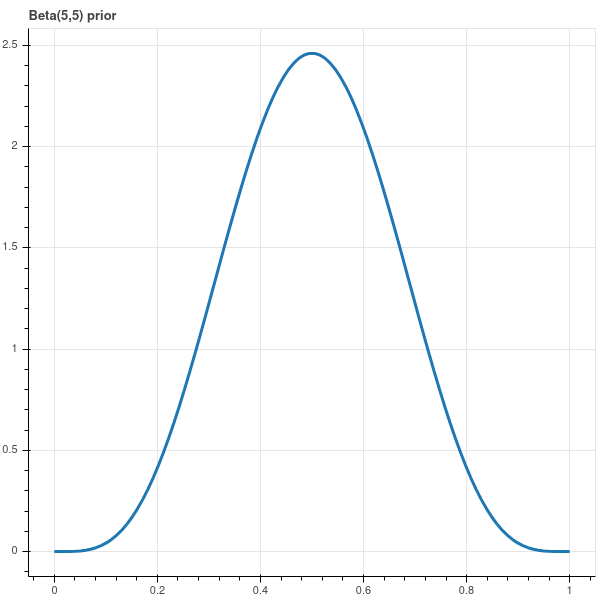
\includegraphics{chapters/img/betaprior.png}

}

\caption{\label{fig-betaprior}Beta(5,5) Prior}

\end{figure}

If we redo our Bayes theorem calculation, we find that our posterior
distribution is \[
P(p|h) \propto p^{h+4}(1-p)^{N-h+4}
\] and relying again on the Beta function for normalization we have \[
P(p|h) = \frac{1}{B(h+5,N-h+5)}p^{h+4}(1-p)^{N-h+4}
\] Here the maximum a posterior estimate for \(p\) is \(h+4/N+8\) while
our posterior mean is \[
\frac{B(h+6,N-h+5)}{B(h+5,N-h+5)} = \frac{h+5}{N+10}.
\]

In the situation of \(55\) heads out of \(100\), the maximum a
posteriori estimate is \(.546\) and the posterior mean is \(.545\).
These numbers have been pulled just a bit towards \(.5\) because our
prior knowledge makes us a little bit biased towards \(p=.5\).

\hypertarget{bayesian-regression-or-ridge-regression}{%
\subsection{Bayesian Regression (or Ridge
Regression)}\label{bayesian-regression-or-ridge-regression}}

In this chapter we return to our discussion of linear regression and
introduce some Bayesian ideas. The combination will lead us to the
notion of ``ridge'' regression, which is a type of linear regression
that includes a prior distribution on the coefficients that indicates
our preference for smaller rather than larger coefficients. Introduction
of this prior leads to a form of linear regression that is more
resilient in situations where the independent variables are less
independent than we would hope.

Before introducing these Bayesian ideas, let us recall from
Section~\ref{sec-LRLike} that ordinary least squares yields the
parameters that give the ``most likely'' set of parameters for a model
of the form \[
Y=XM + \epsilon
\] where the error \(\epsilon\) is normally distributed with mean \(0\)
and variance \(\sigma^2\), and the mean squared error becomes the
maximum likelihood estimate of the variance \(\sigma^2\).

To put this into a Bayesian perspective, we notice that the linear
regression model views \(Y-XM\) as normally distributed given \(M\).
That is, we see the probability \(P(Y-XM|M)\) as normal with variance
\(\sigma^2\).

Then we introduce a prior distribution on the coefficients \(M\),
assuming that they, too, are normally distributed around zero with
variance \(\tau^2\). This means that \emph{ab initio} we think that the
coefficients are likely to be small.

From Bayes Theorem, we then have \[
P(M|Y,X) = \frac{P(Y,X|M)P(M)}{P(Y,X)}
\] and in distribution terms we have \[
P(M|Y,X) = Ae^{\|Y-XM\|^2/\sigma^2}e^{-\|M\|^2/\tau^{2}}
\] where \(A\) is a normalizing constant.

The first thing to note from this expression is that the posterior
distribution for the \(M\) parameters for regression are themselves
normally distributed.

The maximum likelihood estimate \(M_{r}\) for the parameters \(M\)
occurs when \(P(M|Y,X)\) is maximum, which we find by taking the
derivatives. Using the matrix algebra developed in our linear regression
chapter, we obtain the equation \[
(X^{\intercal}Y-(X^{\intercal}X)M_r)/\sigma^2-M_r/\tau^{2}=0
\] or \begin{equation}\protect\hypertarget{eq-ridgeformula}{}{
(X^{\intercal}X+s)M_r=X^{\intercal}Y
}\label{eq-ridgeformula}\end{equation} where \(s=\sigma^2/\tau^2\).

Therefore the ridge coefficients are given by the equation
\begin{equation}\protect\hypertarget{eq-ridgecoeffs}{}{
M_{r}=(X^{\intercal}X+s)^{-1}X^{\intercal}Y
}\label{eq-ridgecoeffs}\end{equation}

\hypertarget{practical-aspects-of-ridge-regression}{%
\subsubsection{Practical aspects of ridge
regression}\label{practical-aspects-of-ridge-regression}}

Using ridge regression leads to a solution to the least squares problem
in which the regression coefficients are biased towards being smaller.
Beyond this, there are a number of implications of the technique which
affect its use in practice.

First, we can put the Bayesian derivation of the ridge regression
formulae in the background and focus our attention on
Equation~\ref{eq-ridgecoeffs}. We can treat the parameter \(s\) (which
must be non-negative) as ``adjustable''.

One important consideration when using ridge regression is that
Equation~\ref{eq-ridgecoeffs} is not invariant if we scale \(X\) and
\(Y\) by a constant. This is different from ``plain'' regression where
we consider the equation \(Y=XM\). In that case, rescaling \(X\) and
\(Y\) by the same factor leaves the coefficients \(M\) alone. For this
reason, ridge regression is typically used on centered, standardized
coordinates. In other words, we replace each feature \(x_i\) by
\((x_i-\mu_i)/\sigma_i\) where \(\mu_i\) and \(\sigma_i\) are the sample
mean and standard deviation of the \(i^{th}\) feature, and we replace
our response variables \(y_i\) similarly by \((y-\mu)/\sigma\) where
\(\mu\) and \(\sigma\) are the mean and standard deviation of the
\(y\)-values. Then we find \(M\) using Equation~\ref{eq-ridgecoeffs},
perhaps experimenting with different values of \(s\), using our centered
and standardized variables.

To emphasize that we are using centered coordinates, we write \(X_{0}\)
for our data matrix instead of \(X\). Recall that the matrix
\(X_0^{\intercal}X_0\) that enters into Equation~\ref{eq-ridgeformula}
is \(ND_{0}\) where \(D_{0}\) is the covariance matrix. Therefore in
ridge regression we have replaced \(ND_0\) by \(ND_0+s\). Since \(D_0\)
is a real symmetric matrix, as we've seen in Chapter 2 it is
diagonalizable so that \(AD_0A^{-1}\) is diagonal for an orthogonal
matrix \(A\) and has eigenvalues \(\lambda_1\ge \ldots\ge \lambda_k\)
which are the variances of the data along the principal directions.

One effect of using ridge regression is that the eigenvalues of
\(ND_{0}+s\) are always at least \(s>0\), so the use of ridge regression
avoids the possibility that \(D_{0}\) might not be invertible. In fact,
a bit more is true. Numerical analysis tells us that when considering
the problem of computing the inverse of a matrix, we should look at its
\emph{condition number}, which is the ratio \(\lambda_1/\lambda_k\) of
the largest to the smallest eigenvalue.

If the condition number of a matrix is large, then results from
numerical analysis show that it is \emph{almost singular} and its
inverse becomes very sensitive to small changes in the entries of the
matrix. However, the eigenvalues of \(ND_0+s\) are \(N\lambda_{i}+s\)
and so the condition number becomes \((N\lambda_1+s)/(N\lambda_k+s)\).
For larger values of \(\lambda\), this condition number shrinks, and so
the inverse of the matrix \(ND_0+s\) becomes better behaved than
\(ND_{0}\). In this way, ridge regression helps to improve the numerical
stability of the linear regression algorithm.

A second way to look at Ridge regression is to go back to the discussion
of the singular value decomposition of the matrix \(X_{0}\) in section
Section~\ref{sec-svd}. There we showed that the SVD of \(X_{0}\) yields
an expression \[
X_{0}=U\tilde{\Lambda}P^{\intercal}
\] where \(U\) and \(P\) are orthogonal matrices and \(\Lambda\) is an
\(N\times k\) matrix whose upper block is diagonal with eigenvalues
\(\sqrt{N\lambda_{i}}\). The rows of \(U\) gave us an orthonormal basis
that allowed us to write the predicted vector \(\hat{Y}\) as a
projection: \[
\hat{Y}=\sum_{i=1}^{k} (u_j\cdot Y)u_{j}^{\intercal}.
\]

If we repeat this calculation, but using the ridge regression formula,
we obtain \[
\hat{Y}_{r}=X_{0}M_r = U\tilde{\Lambda}P^{\intercal}(P\tilde{\Lambda}^{\intercal}U^{\intercal}U\tilde{\Lambda}P^{\intercal}+s)^{-1}P\tilde{\Lambda}^{\intercal}U^{\intercal}Y.
\] Since \(P\) is orthogonal, \(P^{\intercal}=P^{-1}\), so \[
P^{\intercal}(P\tilde{\Lambda}^2P^{\intercal}+s)^{-1}P=P^{-1}(P(\Lambda+s)P^{-1})P=(\Lambda+s)^{-1}
\] and \(\Lambda+s\) is a \(k\times k\) diagonal matrix with entries
\(N\lambda_{i}+s\).

Putting the pieces together we see that \[
\hat{Y}_{r}=U\tilde{\Lambda}(\Lambda+s)^{-1}\tilde{\Lambda}U^{\intercal}Y.
\]

In the language of orthogonal projection, this means that \[
\hat{Y}_{r} = \sum_{i=1}^{k} \frac{N\lambda_{i}}{N\lambda_{i}+s}(u_j\cdot Y)u_{j}^{\intercal}.
\]

In other words, the predicted value computed by ridge regression is
obtained by projecting \(Y\) into the space spanned by the feature
vectors, but weighting the different principal components by
\(N\lambda_{i}/(N\lambda_{i}+s)\). With this weighting, the principal
components with smaller variances are weighted less than those with
larger variances. For this reason, ridge regression is sometimes called
a \emph{shrinkage} method.

\bookmarksetup{startatroot}

\hypertarget{the-naive-bayes-classification-method}{%
\chapter{The Naive Bayes classification
method}\label{the-naive-bayes-classification-method}}

\lstset{columns=fullflexible,breaklines=true,basicstyle=\small\ttfamily,backgroundcolor=\color{gray!10}}

\hypertarget{introduction-2}{%
\section{Introduction}\label{introduction-2}}

In our discussion of Bayes Theorem, we looked at a situation in which we
had a population consisting of people infected with COVID-19 and people
not infected, and we had a test that we could apply to determine which
class an individual belonged to. Because our test was not 100 percent
reliable, a positive test result didn't guarantee that a person was
infected, and we used Bayes Theorem to evaluate how to interpret the
positive test result. More specifically, our information about the test
performance gave us the the conditional probabilities of positive and
negative test results given infection status -- so for example we were
given \(P(+|\mathrm{infected})\), the chance of getting a positive test
assuming the person is infected -- and we used Bayes Theorem to
determine \(P(\mathrm{infected}|+)\), the chance that a person was
infected given a positive test result.

The Naive Bayes classification method is a generalization of this idea.
We have data that belongs to one of two classes, and based on the
results of a series of tests, we wish to decide which class a particular
data point belongs to. For one example, we are given a collection of
product reviews from a website and we wish to classify those reviews as
either ``positive'' or ``negative.'' This type of problem is called
``sentiment analysis.'' For another, related example, we have a
collection of emails or text messages and we wish to label those that
are likely ``spam'' emails. In both of these examples, the ``test'' that
we will apply is to look for the appearance or absence of certain key
words that make the text more or less likely to belong to a certain
class. For example, we might find that a movie review that contains the
word ``great'' is more likely to be positive than negative, while a
review that contains the word ``boring'' is more likely to be negative.

The reason for the word ``naive'' in the name of this method is that we
will derive our probabilities from empirical data, rather than from any
deeper theory. For example, to find the probability that a negative
movie review contains the word ``boring'', we will look at a bunch of
reviews that our experts have said are negative, and compute the
proportion of those that contain the word boring. Indeed, to develop our
family of tests, we will rely on a training set of already classified
data from which we can determine estimates of probabilities that we
need.

\hypertarget{an-example-dataset}{%
\section{An example dataset}\label{an-example-dataset}}

To illustrate the Naive Bayes algorithm, we will work with the
``Sentiment Labelled Sentences Data Set'' ({[}3{]}). This dataset
contains 3 files, each containing 1000 documents labelled \(0\) or \(1\)
for ``negative'' or ``positive'' sentiment. There are 500 of each type
of document in each file. One file contains reviews of products from
amazon.com; one contains yelp restaurant reviews, and one contains movie
reviews from imdb.com.

Let's focus on the amazon reviews data. Here are some samples:

\begin{verbatim}
So there is no way for me to plug it in here 
    in the US unless I go by a converter.   0
Good case, Excellent value. 1
Great for the jawbone.  1
Tied to charger for conversations lasting more than 
    45 minutes.MAJOR PROBLEMS!! 0
The mic is great.   1
I have to jiggle the plug to get it to line up right to 
    get decent volume.  0
If you have several dozen or several hundred contacts, then 
    imagine the fun of sending each of them one by one. 0
If you are Razr owner...you must have this! 1
Needless to say, I wasted my money. 0
What a waste of money and time!.    0
\end{verbatim}

As you can see, each line consists of a product review followed by a
\(0\) or \(1\); in this file the review is separated from the text by a
tab character.

\hypertarget{bernoulli-tests}{%
\section{Bernoulli tests}\label{bernoulli-tests}}

We will describe the ``Bernoulli'' version of a Naive Bayes classifier
for this data. The building block of this method is a test based on a
single word. For example, let's consider the word \textbf{great} among
all of our amazon reviews. It turns out that \textbf{great} occurs \(5\)
times in negative reviews and \(92\) times in positive reviews among our
\(1000\) examples. So it seems that seeing the word \textbf{great} in a
review makes it more likely to be positive. The appearances of great are
summarized in Table~\ref{tbl-great} . We write
\textasciitilde{}\textbf{great} for the case where \textbf{great} does
\emph{not} appear.

\hypertarget{tbl-great}{}
\begin{longtable}[]{@{}llll@{}}
\caption{\label{tbl-great}Ocurrences of \textbf{great} by type of
review}\tabularnewline
\toprule()
& + & - & total \\
\midrule()
\endfirsthead
\toprule()
& + & - & total \\
\midrule()
\endhead
\textbf{great} & 92 & 5 & 97 \\
\textasciitilde{}\textbf{great} & 408 & 495 & 903 \\
total & 500 & 500 & 1000 \\
\bottomrule()
\end{longtable}

In this data, positive and negative reviews are equally likely so
\(P(+)=P(-)=.5\) From this table, and Bayes Theorem, we obtain the
empirical probabilities (or ``naive'' probabilities).

\[
P(\mathbf{great} | +) = \frac{92}{500} = .184
\]

and

\[
P(\mathbf{great}) = \frac{97}{1000} = .097
\]

Therefore

\[
P(+|\mathbf{great}) = \frac{.184}{.097}(.5) = 0.948.
\]

In other words, \emph{if} you see the word \textbf{great} in a review,
there's a 95\% chance that the review is positive.

What if you \emph{do not} see the word \textbf{great}? A similar
calculation from the table yields

\[
P(+|\sim\mathbf{great}) = \frac{408}{903} = .452
\]

In other words, \emph{not} seeing the word great gives a little evidence
that the review is negative (there's a 55\% chance it's negative) but
it's not that conclusive.

The word \textbf{waste} is associated with negative reviews. It's
statistics are summarized in Table~\ref{tbl-waste} .

\hypertarget{tbl-waste}{}
\begin{longtable}[]{@{}llll@{}}
\caption{\label{tbl-waste}Ocurrences of \textbf{waste} by type of
review}\tabularnewline
\toprule()
& + & - & total \\
\midrule()
\endfirsthead
\toprule()
& + & - & total \\
\midrule()
\endhead
\textbf{waste} & 0 & 14 & 14 \\
\textasciitilde{}\textbf{waste} & 500 & 486 & 986 \\
total & 500 & 500 & 1000 \\
\bottomrule()
\end{longtable}

Based on this data, the ``naive'' probabilities we are interested in
are:

\begin{align*}
P(+|\mathbf{waste}) &= 0\\
P(+|\sim\mathbf{waste}) &= .51
\end{align*}

In other words, if you see \textbf{waste} you definitely have a negative
review, but if you don't, you're only slightly more likely to have a
positive one.

What about combining these two tests? Or using even more words? We could
analyze our data to count cases in which both \textbf{great} and
\textbf{waste} occur, in which only one occurs, or in which neither
occurs, within the two different categories of reviews, and then use
those counts to estimate empirical probabilities of the joint events.
But while this might be feasible with two words, if we want to use many
words, the number of combinations quickly becomes huge. So instead, we
make a basic, and probably false, assumption, but one that makes a
simple analysis possible.

\textbf{Assumption:} We assume that the presence or absence of the words
\textbf{great} and \textbf{waste} in a particular review (positive or
negative) are independent events. More generally, given a collection of
words \(w_1,\ldots, w_k\), we assume that their occurences in a given
review are independent events.

Independence means that we have \begin{align*}
P(\mathbf{great},\mathbf{waste}|\pm) &= P(\mathbf{great}|\pm)P(\mathbf{waste}|\pm)\\
P(\mathbf{great},\sim\mathbf{waste}|\pm) &= P(\mathbf{great}|\pm)P(\sim\mathbf{waste}|\pm)\\
 &\vdots \\
\end{align*}

So for example, if a document contains the word \textbf{great} and does
\emph{not} contain the word \textbf{waste}, then the probability of it
being a positive review is: \[
P(+|\mathbf{great},\sim\mathbf{waste}) = \frac{P(\mathbf{great}|+)P(\sim\mathbf{waste}|+)P(+)}{P(\mathbf{great},\sim\mathbf{waste})}
\] while the probability of it being a negative review is \[
P(-|\mathbf{great},\sim\mathbf{waste}) = \frac{P(\mathbf{great}|-)P(\sim\mathbf{waste}|-)P(-)}{P(\mathbf{great},\sim\mathbf{waste})}
\] Rather than compute these probabilities (which involves working out
the denominators), let's just compare them. Since they have the same
denominators, we just need to compare numerators, which we call \(L\)
for likelihood: Using the data from Table~\ref{tbl-great} and
Table~\ref{tbl-waste} , we obtain: \[
L(+|\mathbf{great},\sim\mathbf{waste}) = (.184)(1)(.5) = .092
\] and \[
L(-|\mathbf{great},\sim\mathbf{waste}) = (.01)(.028)(.5) = .00014
\] so our data suggests strongly that this is a positive review.

\hypertarget{feature-vectors}{%
\section{Feature vectors}\label{feature-vectors}}

To generalize this, suppose that we have extracted keywords
\(w_1,\ldots, w_k\) from our data and we have computed the empirical
values \(P(w_{i}|+)\) and \(P(w_{i}|-)\) by counting the fraction of
positive and negative reviews that contain the word \(w_{i}\):

\[
P(w_{i}|\pm) = \frac{\hbox{ number of $\pm$ reviews that mention $w_{i}$}}{\hbox{ number of $\pm$ reviews total}}
\]

Notice that we only count \emph{reviews}, not \emph{ocurrences}, so that
if a word occurs multiple times in a review it only contributes 1 to the
count. That's why this is called the \emph{Bernoulli} Naive Bayes -- we
are thinking of each keyword as yielding a yes/no test on each review.

Given a review, we look to see whether each of our \(k\) keywords
appears or does not. We encode this information as a vector of length
\(k\) containing \(0\)'s and \(1\)'s indicating the absence or presence
of the \(k\)th keyword. Let's call this vector the \emph{feature vector}
for the review.

For example, if our keywords are \(w_1=\mathbf{waste}\),
\(w_2=\mathbf{great}\), and \(w_3=\mathbf{useless}\), and our review
says

\begin{verbatim}
This phone is useless, useless, useless!  What a waste!
\end{verbatim}

then the associated feature vector is \(f=(1,0,1)\).

For the purposes of classification of our reviews, we are going to
forget entirely about the text of our reviews and work only with the
feature vectors. From an abstract perspective, then, by choosing our
\(k\) keywords, our ``training set'' of \(N\) labelled reviews can be
replaced by an \(N\times k\) matrix \(X=(x_{ij})\) with entries \(0\) or
\(1\), where \(x_{ij}=1\) if and only if the \(j^{th}\) keyword appears
in the \(i^{th}\) review.

The labels of \(0\) or \(1\) for unfavorable or favorable reviews can
also be packaged up into a \(N\times 1\) vector \(Y\) that serves as our
``target'' variable.

Setting things up this way lets us express the computations of our
probabilities \(P(w_{i}|\pm)\) in vector form. In fact,
\(Y^{\intercal}X\) is the sum of the rows of \(X\) corresponding to
positive reviews, and therefore, letting \(N_{\pm}\) denote the number
of \(\pm\) reviews, \[
P_{+} = \frac{1}{N_{+}}Y^{\intercal}X = \left[\begin{array}{cccc} P(w_{1}|+)& P(w_{2}|+) & \cdots &P(w_{k}|+)\end{array}\right].
\] Similarly, since \(Y\) and \(X\) have zero and one entries only, if
we write \(1-Y\) and \(1-X\) for the matrices obtained by replacing
every entry \(z\) by \(1-z\) in each matrix, we have: \[
P_{-} = \frac{1}{N_{-}}(1-Y)^{\intercal}X =  \left[\begin{array}{cccc} P(w_{1}|-)& P(w_{2}|-) & \cdots &P(w_{k}|-)\end{array}\right].
\]

Note that the number of positive reviews is \(N_{+}=Y^{\intercal}Y\) and
the number of negative ones is \(N_{-}=N-N_{+}\). Since \(P(+)\) is the
fraction of positive reviews among all reviews, we can compute it as
\(P(+)=\frac{1}{N}Y^{\intercal}Y\), and \(P(-)=1-P(+)\).

\hypertarget{likelihood}{%
\section{Likelihood}\label{likelihood}}

If a review has an associated feature vector \(f=(f_1,\ldots, f_k)\),
then by independence the probability of that feature vector ocurring
within one of the \(\pm\) classes is \[
P(f|\pm) = \prod_{i: f_{i}=1} P(w_{i}|\pm)\prod_{i: f_{i}=0}(1-P(w_{i}|\pm))
\] which we can also write
\begin{equation}\protect\hypertarget{eq-likelihood}{}{
P(f|\pm) = \prod_{i=1}^{k} P(w_{i}|\pm)^{f_{i}}(1-P(w_{i}|\pm))^{(1-f_{i})}.
}\label{eq-likelihood}\end{equation}

These products aren't practical to work with -- they are often the
product of many, many small numbers and are therefore really tiny.
Therefore it's much more practical to work with their logarithms.
\begin{equation}\protect\hypertarget{eq-loglikelihood}{}{
\log P(f|\pm) = \sum_{i=1}^{k} f_{i}\log P(w_{i}|\pm) + (1-f_{i})\log(1-P(w_{i}|\pm))
}\label{eq-loglikelihood}\end{equation}

If we have a group of reviews \(N\) organized in a matrix \(X\), where
each row is the feature vector associated to the corresponding review,
then we can compute all of this at once. We'll write
\(\log P_{\pm}=\log P(X|\pm)\) as the row vector whose \(i^{th}\) entry
is \(\log P(f_{i}|\pm)\):

\begin{equation}\protect\hypertarget{eq-matrixlikelihood}{}{
\log P(X|\pm) = X(\log P_{\pm})^{\intercal}+(1-X)(\log (1-P_{\pm}))^{\intercal}.
}\label{eq-matrixlikelihood}\end{equation}

By Bayes Theorem, we can express the chance that our review with feature
vector \(f\) is positive or negative by the formula: \[
\log P(\pm|f) = \log P(f|\pm)+\log P(\pm) - \log P(f)
\] where \[
P(\pm) = \frac{\hbox{ the number of $\pm$ reviews}}{\hbox{ total number of reviews}}
\] and \(P(f)\) is the fraction of reviews with the given feature
vector. (Note: in practice, some of these probabilities will be zero,
and so the log will not be defined. A common practical approach to
dealing with this is to introduce a ``fake document'' into both classes
in which every vocabulary word appears -- this guarantees that the
frequency matrix will have no zeros in it).

A natural classification rule would be to say that a review is positive
if \(\log P(+|f)>\log P(-|f)\), and negative otherwise. In applying
this, we can avoid computing \(P(f)\) by just comparing
\(\log P(f|+)+\log P(+)\) and \(\log P(f|-)+\log P(-)\) computed using
Equation~\ref{eq-loglikelihood}. Then we say:

\begin{itemize}
\tightlist
\item
  a review is positive if
  \(\log P(f|+)+\log P(+)>\log P(f|-)+\log P(-)\) and negative
  otherwise.
\end{itemize}

Again we can exploit the matrix structure to do this for a bunch of
reviews at once. Using Equation~\ref{eq-matrixlikelihood} and the
vectors \(P_{\pm}\) we can compute column vectors corresponding to both
sides of our decision inequality and subtract them. The positive entries
indicate positive reviews, and the negative ones, negative reviews.

\hypertarget{the-bag-of-words}{%
\section{The Bag of Words}\label{the-bag-of-words}}

In our analysis above, we thought of the presence or absence of certain
key words as a set of independent tests that provided evidence of
whether our review was positive or negative. This approach is suited to
short pieces of text, but what about longer documents? In that case, we
might want to consider not just the presence or absence of words, but
the frequency with which they appear. Multinomial Naive Bayes, based on
the ``bag of words'' model, is a classification method similar to
Bernoulli Naive Bayes but which takes term frequency into account.

Let's consider, as above, the problem of classifying documents into one
of two classes. We assume that we have a set of keywords
\(w_1,\ldots, w_k\). For each class \(\pm\), we have a set of
probabilities \(P(w_i|\pm)\) with the property that \[
\sum_{i=1}^{k}P(w_{i}|\pm)=1.
\]

The ``bag of words'' model says that we construct a document of length
\(N\) in, say, the \(+\) class by independently drawing a word \(N\)
times from the set \(w_1,\ldots, w_k\) with probabilities
\(P(w_{i}|+)\). The name ``bag of words'' comes from thinking of each
class as having an associated bag containing the words
\(w_1,\ldots, w_k\) with relative frequencies given by the
probabilities, and generating a document by repeatedly drawing a word
from the bag.

In the Multinomial Naive Bayes method, we estimate the probabilities
\(P(w_{i}|\pm)\) by counting the number of times each word occurs in a
document of the given class: \[
P(w_{i}|\pm) = \frac{\hbox{ number of times word $i$ occurs in $\pm$ documents}}{\hbox{ total number of words in $\pm$ documents}}
\] This is the ``naive'' part of the algorithm. Package up these
probabilities in vectors: \[
P_{\pm} = \left[\begin{array}{ccc} P(w_{1}|\pm) & \cdots & P(w_{k}|\pm)\end{array}\right].
\]

As in the Bernoulli case, we often add a fake document to each class
where all of the words occur once, in order to avoid having zero
frequencies when we take a logarithm later.

Now, given a document, we associate a feature vector \(\mathbf{f}\)
whose \(i^{th}\) entry is the frequency with which word \(i\) appears in
that document. The probability of obtaining a particular document with
feature vector \(\mathbf{f}=(f_1,\ldots, f_k)\) from the bag of words
associated with class \(\pm\) is given by the ``multinomial''
distribution: \[
P(\mathbf{f}|\pm)=\frac{N!}{f_1!f_2!\cdots f_k!} \prod_{i=1}^{k} P(w_{i}|\pm)^{f_{i}}
\] which generalizes the binomial distribution to multiple choices. The
constant will prove irrelevant, so let's call the interesting part
\(L_{\pm}\): \[
L(\mathbf{f}|\pm)= \prod_{i=1}^{k} P(w_{i}|\pm)^{f_{i}}
\]

From Bayes Theorem, we have \[
P(\pm|\mathbf{f}) = \frac{P(\mathbf{f}|\pm)P(\pm)}{P(\mathbf{f})}
\] where \(P(\pm)\) is estimated by the fraction of documents (total) in
each class.

We classify our document by considering \(P(\pm|\mathbf{f})\) and
concluding:

\begin{itemize}
\tightlist
\item
  a document with feature vector \(\mathbf{f}\) is in class \(+\) if
  \(\log P(+|\mathbf{f})>\log P(-|\mathbf{f})\).
\end{itemize}

In this comparison, both the constant (the multinomial coefficient) and
the denominator cancel out, so we only need to compare
\(\log L(\mathbf{f}|+)+\log P(+)\) with
\(\log L(\mathbf{f}|-)+\log P(-)\) We have \[
\log L(\mathbf{f}|\pm) = \sum_{i=1}^{k} f_{i}\log P(w_{i}|\pm)
\] or, in vector form, \[
\log P(\mathbf{f}|\pm) = \mathbf{f}\log P_{\pm}^{\intercal}
\]

Therefore, just as in the Bernoulli case, we can package up our document
\(i\) as an \(N\times k\) data matrix \(X\), where position \(ij\) gives
the number of times word \(j\) occurs in document \(i\). Then we can
compute the vector \[
\hat{Y} = X\log P_{+}^{\intercal} + \log P(+)-X\log P_{-}^{\intercal} - \log P(-)
\] and assign those documents where \(\hat{Y}>0\) to the \(+\) class and
the rest to the \(-\) class.

\hypertarget{other-applications}{%
\section{Other applications}\label{other-applications}}

We developed the Naive Bayes method for sentiment analysis, but once we
chose a set of keywords our training data was reduced to an
\(N\times k\) matrix \(X\) of \(0/1\) entries, together with an
\(N\times 1\) target column vector \(Y\). Then our classification
problem is to decide whether a given vector of \(k\) entries, all \(0\)
or \(1\), is more likely to carry a \(0\) or \(1\) label. All of the
parameters we needed for Naive Bayes -- the various probabilities -- can
be extracted from the matrix \(X\).

For example, suppose we have a collection of images represented as
black/white pixels in a grid that belong to one of two classes. For
example, we might have \(28x28\) bitmaps of handwritten zeros and ones
that are labelled, and we wish to construct a classifier that can decide
whether a new \(28x28\) bitmap is a zero or one. An example of such a
bitmap is given in Figure~\ref{fig-mnist0}. We can view each \(28x28\)
bitmap as a vector of length \(784\) with \(0/1\) entries and apply the
same approach outlined above. However, there are other methods that are
more commonly used for this problem, such as logistic regression and
neural networks.

\begin{figure}

{\centering 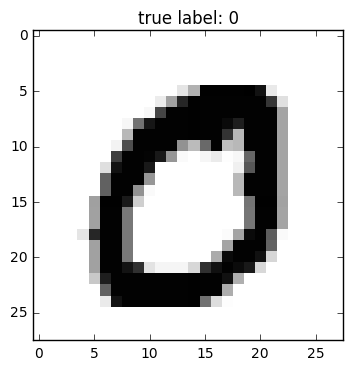
\includegraphics[width=2in,height=\textheight]{chapters/img/mnist_data_10_0.png}

}

\caption{\label{fig-mnist0}Handwritten 0}

\end{figure}

\bookmarksetup{startatroot}

\hypertarget{sec-gradient_descent}{%
\chapter{Gradient Descent}\label{sec-gradient_descent}}

\[\newcommand{\df}[1]{\frac{\partial}{\partial #1}}\]
\[\newcommand{\R}{\mathbf{R}}\]

\hypertarget{introduction-3}{%
\section{Introduction}\label{introduction-3}}

A common mathematical theme throughout machine learning is the problem
of finding the minimum or maximum value of a function. For example, in
linear regression, we find the ``best-fitting'' linear function by
identifying the parameters that minimize the mean squared error. In
principal component analysis, we try to identify the scores which have
the greatest variation for the given set of data, and for this we needed
to maximize a function using Lagrange multipliers. In later lectures, we
will see many more examples where we construct the ``best'' function for
a particular task by minimizing some kind of error between our
constructed function and the true observed values.

In our discussion of PCA and linear regression, we were able to give
analytic formulae for the solution to our problems. These solutions
involved (in the case of linear regression) inverting a matrix, and in
the case of PCA, finding eigenvalues and eigenvectors. These are elegant
mathematical results, but at that time we begged the question of how to
actually \emph{compute} these quantities of interest in an efficient
way. In this section, we will discuss the technique known as gradient
descent, which is perhaps the simplest approach to minimizing a function
using calculus, and which is at the foundation of many practical machine
learning algorithms.

\hypertarget{the-key-idea}{%
\section{The Key Idea}\label{the-key-idea}}

Suppose that we have a function \(f(x_0,\ldots, x_{k-1})\) and we wish
to find its minimum value. In Calculus classes, we are taught to take
the derivates of the function and set them equal to zero, but for
anything other than the simplest functions this problem is not solvable
in practice. In real life, we use iterative methods to find the minimum
of the function \(f\).

The main tool in this approach is a fact from multivariate calculus.

\textbf{Proposition:} Let \(f(x_0,\ldots, x_{k-1})\) be a function and
let \(\nabla f\) be its gradient. Then at each point \(x\) in
\(\R^{k}\), the gradient \((\nabla f)(x)\) is a vector that points in
the direction in which \(f\) is increasing most rapidly from \(x\) and
\((-\nabla f)(x)\) points is a critical point of \(f\).

This fact arises from thinking about the \emph{directional derivative}
of a function.\\
The directional derivative \(D_{v}f\) measures the rate of change of
\(f\) as one moves with velocity vector \(v\) from the point \(x\) and
it is defined as \[
D_{v}f(x) = \frac{d}{dt}f(x+tv)|_{t=0}
\] From the chain rule, we can compute that \[
D_{v}f(x) = \sum_{i=0}^{k-1} \frac{\partial f}{\partial x_{i}}\frac{dx_{i}}{dt} = (\nabla f)\cdot v
\] where \[
\nabla f = \left[\frac{\partial f}{\partial x_{i}}\right]_{i=0}^{k-1}
\] is the gradient of \(f\).

The directional derivative \(D_{v}(f)=(\nabla f)\cdot v\) measures the
rate of change of \(f\) if we travel with velocity \(v\) from a point
\(x\). To remove the dependence on the magnitude of \(v\) (since
obviously \(f\) will change more quickly if we travel more quickly in a
given direction), we scale \(v\) to be a unit vector. Then, since \[
\nabla f\cdot v=\|\nabla f\|\|v\|\cos\theta=\|\nabla f\|\cos \theta
\] where \(\theta\) is the angle between \(v\) and \(\nabla f\), the dot
product giving the rate is maximized when \(v\) is parallel to
\(\nabla f\). If \(v\) is opposite to \(\nabla f\), the dot product is
minimized.

\hypertarget{the-algorithm}{%
\section{The Algorithm}\label{the-algorithm}}

To exploit the fact that the gradient points in the direction of most
rapid increase of our function \(f\), we adopt the following strategy.
Starting from a point \(x\), compute the gradient \(\nabla f\) of \(f\).
Take a small step in the direction of the gradient -- that should
increase the value of \(f\). Then do it again, and again; each time, you
move in the direction of increasing \(x\), but at some point the
gradient becomes very small and you stop moving much. At that moment,
you quit. This is called ``gradient ascent.''

If we want to \emph{minimize}, not maximize, our function, then we want
to move \emph{opposite} to the gradient in small steps. This is the more
common formulation.

\leavevmode\vadjust pre{\hypertarget{alg-gradient_descent}{}}%
\begin{algorithm}[Gradient Descent
Algorithm]\label{alg-gradient_descent}

Given a function \(f:\mathbb{R}^{k}\to \mathbb{R}\), to find a point
where it is mimized, choose:

\begin{itemize}
\tightlist
\item
  a starting point \(c^{(0)}\),
\item
  a small constant \(\nu\) (called the \emph{learning rate})
\item
  and a small constant \(\epsilon\) (the \emph{tolerance}).
\end{itemize}

Iteratively compute \[
c^{(n+1)}=c^{(n)} -\nu\nabla f(c^{(n)})
\] until \(|c^{(n+1)}-c^{(n)}|<\epsilon\).

Then \(c^{(n+1)}\) is an (approximate) critical point of \(f\).

\end{algorithm}

\begin{figure}

{\centering 

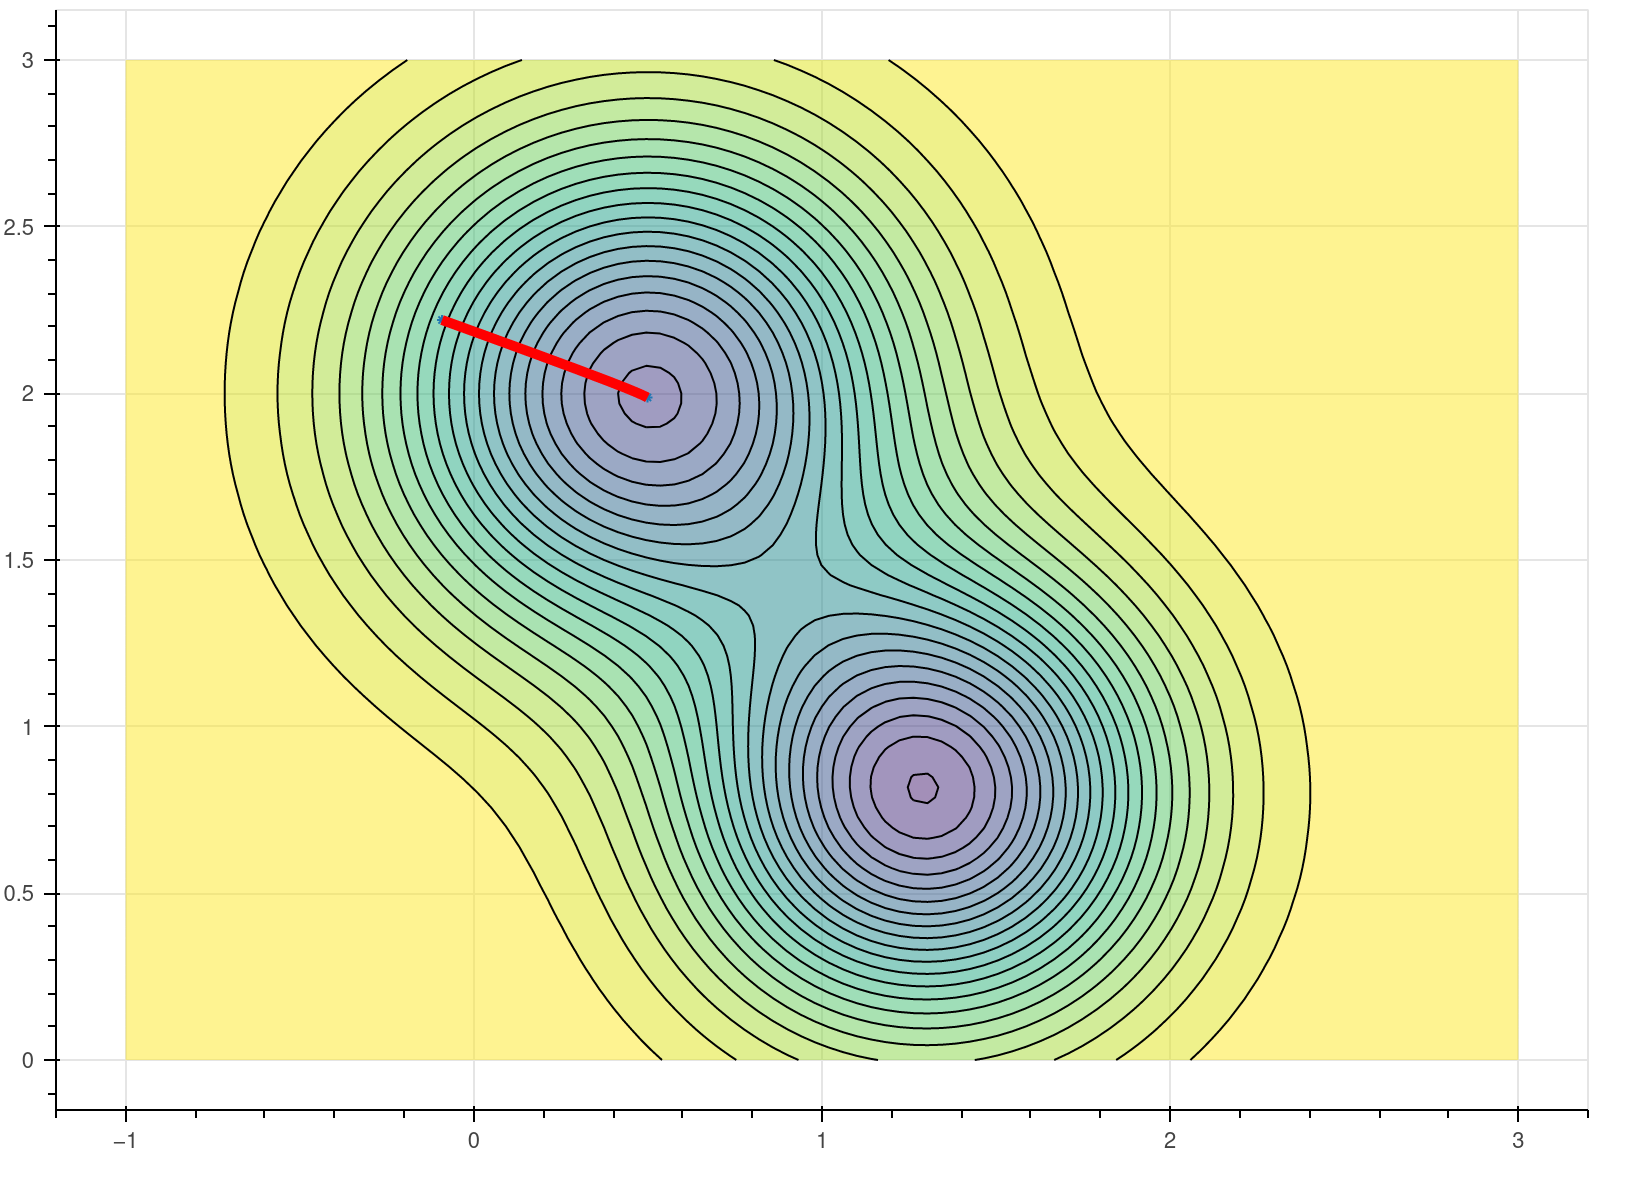
\includegraphics{chapters/img/gradient_descent.png}

}

\caption{\label{fig-graddescentillust}Gradient Descent Illustrated}

\end{figure}

The behavior of gradient descent, at least when all goes well, is
illustrated in Figure~\ref{fig-graddescentillust} for the function \[
f(x,y) = 1.3e^{-2.5((x-1.3)^2+(y-0.8)^2))}-1.2e^{-2((x-1.8)^2)+(y-1.3)^2)}.
\] Figure~\ref{fig-graddescentillust} is a contour plot, with the black
lines at constant height and the colors indicating the height of the
function. This function has two ``pits'' or ``wells'' indicated by the
darker, ``cooler'' colored regions. The red line shows the path that the
gradient descent algorithm takes, from a higher, ``hotter'' region to a
lower cooler one.

To get a little more perspective on gradient descent, consider the
one-dimensional case, with \[
f(x)=3x^4+4x^3-12x^2+5.
\] This is a quartic polynomial whose graph has two local minima and a
local maximum, depicted in Figure~\ref{fig-graddescentquartic}.

\begin{figure}

{\centering 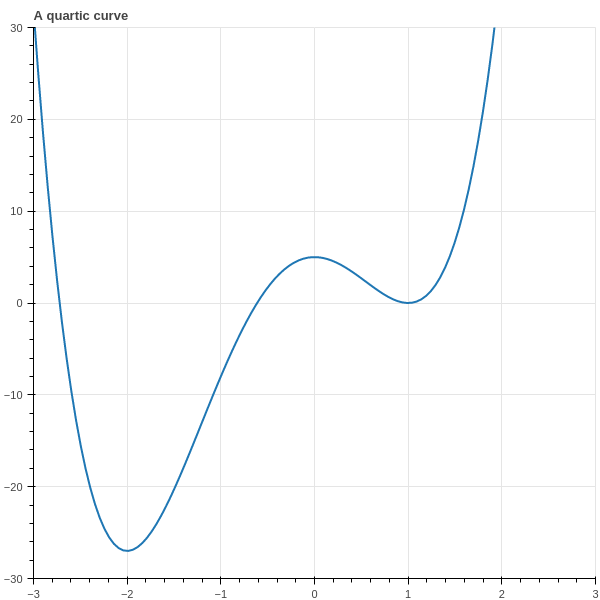
\includegraphics[width=0.5\textwidth,height=\textheight]{chapters/img/GradDescentQuartic.png}

}

\caption{\label{fig-graddescentquartic}A quartic polynomial}

\end{figure}

In this case the gradient is just the derivative \[
f'(x)=12x^3+12x^2-24x
\] and the iteration is \[
c^{(n+1)} = c^{(n)}-12\nu((c^{(n)})^3+(c^{(n)})^2-2c^{(n)}).
\]

From this simple example we can see the power and also the pitfalls of
this method. Suppose we choose \(x_0=.5\), \(\nu=.01\), and do \(30\)
iterations of the main loop in our algorithm. The result is shown in
Figure~\ref{fig-grad_descent_local_minimum} .

\begin{figure}

{\centering 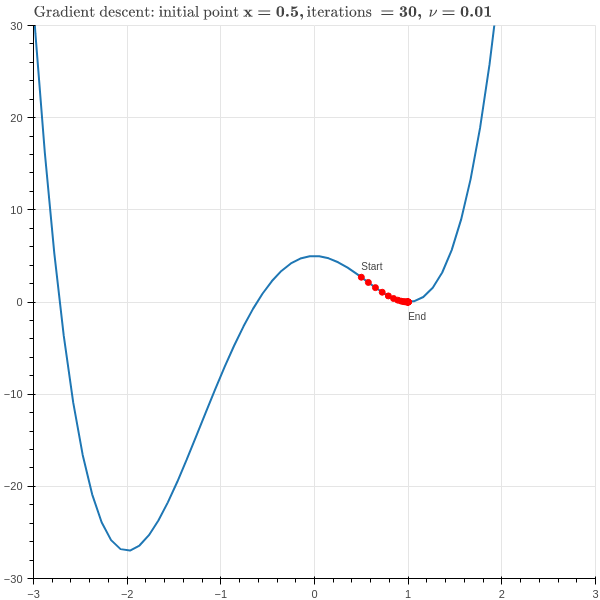
\includegraphics{chapters/img/grad_descent_local_minimum.png}

}

\caption{\label{fig-grad_descent_local_minimum}Gradient descent to a
local minimum}

\end{figure}

As we hope, the red dots quickly descend to the bottom of the ``valley''
at the point \(x=1\). However, this valley is only a \emph{local
minimum} of the function; the true minimum is at \(x=-2\). Gradient
descent can't see that far away point and so we don't find the true
minimum of the function. One way to handle this is to \emph{run gradient
descent multiple times with random starting coordinates} and then look
for the minimum value it finds among all of these tries.

\hypertarget{linear-regression-via-gradient-descent}{%
\section{Linear Regression via Gradient
Descent}\label{linear-regression-via-gradient-descent}}

In our discussion of Linear Regression in
Chapter~\ref{sec-LinearRegression}, we used Calculus to find the values
of the parameters that minimzed the squared difference to the desired
values. If our features were stored in the matrix \(X\) (with an
additional column of \(1\)'s) and our target values in the vector \(Y\),
then we showed that that optimal parameters \(M\) were given by

\[
M=D^{-1}X^{\intercal}Y
\]

where \(D=X^{\intercal}X\). This set of parameters minimizes the
``mean-squared-error''

\[
MSE = \frac{1}{N}\| Y-XM \|^2.
\]

See Equation~\ref{eq-Msolution} and Equation~\ref{eq-projection}.

One problem with this approach is the need to invert the matrix \(D\),
which is a serious computation in its own right. We can avoid relying on
matrix inversion by approaching this problem numerically via gradient
descent, using the computation of the gradient in
Equation~\ref{eq-gradient}:

\[ 
\nabla E = \left[\begin{matrix} \df{M_1}E \\ \df{M_2}E \\ \vdots \\
\df{m_{M+1}}E\end{matrix}\right] = -2 X^{\intercal}Y + 2
X^{\intercal}XM 
\]

The gradient descent algorithm looks like this.

\leavevmode\vadjust pre{\hypertarget{alg-graddescentLinearRegression}{}}%
\begin{algorithm}[Gradient Descent Algorithm for Linear
Regression]\label{alg-graddescentLinearRegression}

Set \(M^{0}\) to a random vector in \(\R^{k+1}\) for an initial guess
and choose a learning rate parameter \(\nu\). Compute
\(A=X^{\intercal}Y\) (an element of \(\R^{k+1}\) and
\(D=X^{\intercal}X\) (a \((k+1)\times (k+1)\) matrix).

Iteratively compute

\[
M^{(j+1)}=M^{(j)}-\nu(-2A+2DM^{(j)})
\]

until the entries a stopping condition is met. For example, stop if the
mean squared error \(\|Y-XM^{(k)}\|^2\) changes by less than some
tolerance on each iteration, or the entries of \(M^{(k)}\) change by
less than some tolerance.

\end{algorithm}

Notice that this algorithm does not need computation of \(D^{-1}\).

\hypertarget{stochastic-gradient-descent-sec-sgd}{%
\section{\texorpdfstring{Stochastic Gradient Descent
\{\textbf{?@sec-sgd}\}}{Stochastic Gradient Descent \{?@sec-sgd\}}}\label{stochastic-gradient-descent-sec-sgd}}

Using the numerical approach to linear regression avoids computing
\(D^{-1}\), but still leaves us the task of computing the matrix
\(D=X^{\intercal}X\). Typically \(X\) has many rows, and so this
computation is time intensive. We would like to avoid having to use
\emph{all} of the data for each iteration of our algorithm.

Stochastic Gradient Descent is a method for numerical optimization that
does not require use of all the data on each iteration; rather it uses
each data point in succession. Let's look at this in the context of
linear regression. Suppose we have an estimated value \(M\) for the
parameters. We take one data point \(x\) -- a single row of the data
matrix \(X\) -- and the associated target value \(y\). The MSE error for
this particular point is

\[
MSE = \| (y-xM)\|^2 = (y-xM)\cdot (y-xM).
\]

The gradient for this particular point is

\[
\nabla MSE = -2(y-xM)x
\]

Notice that \(y-xM\) is just a scalar so this is a scalar multiple of
the vector \(x\).

Now we iterate over the data, adjusting the parameters \(M\) by this
partial gradient. Each pass through the entire set is sometimes called
an ``epoch.''

\leavevmode\vadjust pre{\hypertarget{alg-stochastic-sgd}{}}%
\begin{algorithm}[Stochastic Gradient Descent for Linear
Regression]\label{alg-stochastic-sgd}

Set \(M^{0}\) to a random starting vector in \(\R^{k+1}\) as an initial
guess and choose a learning rate parameter.

For each data point \(x\) and target value \(y\), adjust the parameters
by the gradient of the error associated with this point:

\[
M^{(j+1)} = M^{(j)}-\nu(-2x(y-xM)) = M^{(j)}+2\nu(y-xM)x
\]

Run through the data set multiple times and track the \(MSE\)
\(\|(y-xM)\|^2\) for each pair \((x,y)\). These will bounce around but
trend overall downward. When they vary by less than some threshold,
stop.

\textbf{Note:} To minimize the bias introduced by the particular order
in which you read the data, it's often worthwhile to shuffle the order
in which you consider the points \((x,y)\) in each epoch.

\end{algorithm}

\bookmarksetup{startatroot}

\hypertarget{logistic-regression}{%
\chapter{Logistic Regression}\label{logistic-regression}}

Suppose that we are trying to convince customers to buy our product by
showing them advertising. Our experience teaches us that there is no
deterministic relationship between how often a potential customer sees
one of our ads and whether or not they purchase our product,
nevertheless it is the case that as they see more ads they become more
likely to make a purchase. Logistic regression is a statistical model
that captures this idea.

To formulate this situation mathematically, let's imagine that we are
trying to model a random event that depends on a parameter. The random
event might be a user deciding to make a purchase from a website, which,
in our very simple model, depends on how many times the user saw an
advertisement for the product in question. But we could imagine other
situations where the chance of an event happening depends on a
parameter. For example, we could imagine that a student's score on a
certain test depends on how much studying they do, with the likelihood
of passing the test increasing with the amount of studying.

To construct this model, we assume that the probability of a certain
event \(p\) is related to some parameter \(x\) by the following
relationship:

\begin{equation}\protect\hypertarget{eq-logistic_1}{}{
\log\frac{p}{1-p} = ax+b 
}\label{eq-logistic_1}\end{equation}

where \(a\) and \(b\) are constants. The quantity \(\frac{p}{1-p}\) is
the ``odds'' of the event occurring. We often use this quantity
colloquially; if the chance of our team winning a football game is \(1\)
in \(3\), then we would say the odds of a win are \(1\)-to-\(2\), which
we can interpret as meaning they are twice as likely to lose as to win.
The quantity \(\log\frac{p}{1-p}\) is, for obvious reasons, called the
log-odds of the event. The logistic model in
Equation~\ref{eq-logistic_1} means that an increase by \(1\) in the
parameter \(x\) increases the log-odds of the event happening by \(a\).

The assumption in Equation~\ref{eq-logistic_1} can be written \[
\frac{p}{1-p} = e^{ax+b}
\] and we interpret this as telling us that if the parameter \(x\)
increases by \(1\), the odds of our event happening go up by a factor of
\(e^{a}\). So, to be even more concrete, if \(a=\log 2\), then our
logistic model would say that an increase of \(1\) in our parameter
\(x\) doubles the odds of our event taking place.

In terms of the probability \(p\), Equation~\ref{eq-logistic_1} can be
rewritten \[
p = \frac{1}{1+e^{-ax-b}}
\] This proposed relationship between the probability \(p\) and the
parameter \(x\) is called the \emph{logistic model.} The function \[
\sigma(x) = \frac{1}{1+e^{-x}}
\] is called the \emph{logistic function} and yields an S-shaped curve.

\begin{figure}

{\centering 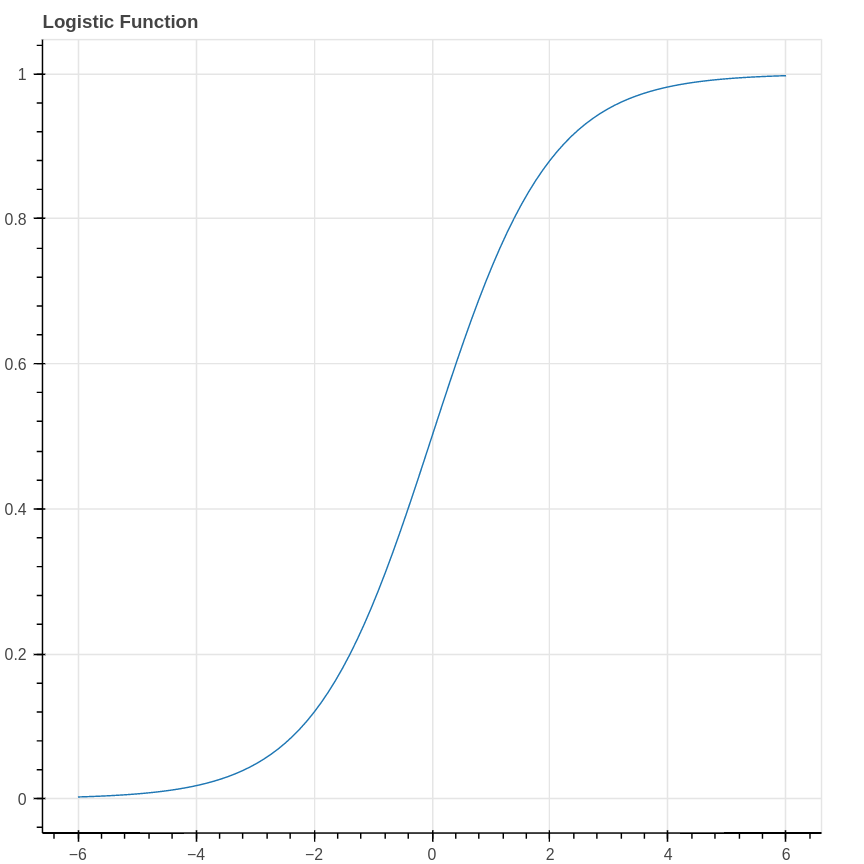
\includegraphics[width=0.5\textwidth,height=\textheight]{chapters/img/logistic_curve.png}

}

\caption{\label{fig-logistic_curve}Logistic Curve}

\end{figure}

To put the logistic model in perspective, let's choose some explicit
parameters and look at what data arising from such a model would look
like. Imagine therefore that \(a=\log 2\) and \(b=0\), so that the
probability of the event we are interested occurring is given by the
formula \[
p(x) = \frac{1}{1+e^{-(\log 2)x}} = \frac{1}{1+(.5)^x}.
\] Our data consists of counts of how often our event happened for a
range of values of \(x\). To generate this data, we can pick \(x\)
values from the set \(\{-3,-2,-1,0,1,2,3\}\) yielding probabilities
\(\{.11,.2,.33,.4,.56,.67,.8\}\). Now our data consists of, for each
value of \(x\), the result of \(100\) independent Bernoulli trials with
probability \(p(x)\). For example, we might find that our event occurred
\(\{10, 18, 38, 50, 69, 78, 86\}\) times respectively for each of the
\(x\) values. As you can see, the event occurs more frequently when
\(x\) is large, although the number of occurrences is still random.

\hypertarget{likelihood-and-logistic-regression}{%
\section{Likelihood and Logistic
Regression}\label{likelihood-and-logistic-regression}}

In applications, our goal is to choose the parameters of a logistic
model to accurately predict the likelihood of the event under study
occurring as a function of the measured parameter. Let's imagine that we
collected the data that we generated above, without knowing that it's
source was a logistic model. So Table~\ref{tbl-logistic_data} shows the
number of times the event occurred, for each of the measured values of
the \(x\) parameter.

\hypertarget{tbl-logistic_data}{}
\begin{longtable}[]{@{}llllllll@{}}
\caption{\label{tbl-logistic_data}Sample Data}\tabularnewline
\toprule()
\(x\) & -3 & -2 & -1 & 0 & 1 & 2 & 3 \\
\midrule()
\endfirsthead
\toprule()
\(x\) & -3 & -2 & -1 & 0 & 1 & 2 & 3 \\
\midrule()
\endhead
Occurrences (out of 100) & 10 & 18 & 38 & 50 & 69 & 78 & 86 \\
\bottomrule()
\end{longtable}

Our objective now is to find a logistic model which best explains this
data. Concretely, we need to estimate the coefficients \(a\) and \(b\)
that yield \begin{equation}\protect\hypertarget{eq-logistic_a_b}{}{
p(x) = \frac{1}{1+e^{-ax-b}}
}\label{eq-logistic_a_b}\end{equation}

where the resulting probabilities best estimate the data. As we have
seen, this notion of ``best'' can have different interpretations. For
example, we could approach this from a Bayesian point of view, adopt a
prior distribution on the parameters \(a\) and \(b\), and use the data
to obtain this prior and obtain a posterior distribution on \(a\) and
\(b\). For this first look at logistic regression, we will instead adopt
a ``maximum likelihood'' notion of ``best'' and ask what is the most
likely choice of \(a\) and \(b\) to yield this data.

To apply the maximum likelihood approach, we need to ask ``for (fixed,
but unknown) values of \(a\) and \(b\), what is the likelihood that a
logistic model with those parameters would yield the data we have
collected?'' Each column in Table~\ref{tbl-logistic_data} represents
\(100\) Bernoulli trials with a fixed probability \(p(x)\). So, for
example, the chance \(q\) of obtaining \(10\) positive results with
\(x=-3\) is given by \[
q(-3)=C p(-3)^{10}(1-p(-3))^{90}
\] where \(C\) is a constant (it would be a binomial coefficient).
Combining this for different values of \(x\), we see that the likelihood
of the data is the product \[
L(a,b) = C' p(-3)^{10}(1-p(-3))^{90}p(-2)^{18}(1-p(-2))^{82}\cdots p(3)^{86}(1-p(3))^{14}
\] where \(C'\) is another constant. Each \(p(x)\) is a function of the
parameters \(a\) and \(b\), so all together this is a function of those
two parameters. Our goal is to maximize it.

One step that simplifies matters is to consider the logarithm of the
likelihood: \[
\log L (a,b)= \sum_{i=0}^{6} \left[ x_{i}\log(p(x_{i})) + (100-x_{i})\log(1-p(x_{i}))\right] +C''
\] where \(C''\) is yet another constant. Since our ultimate goal is to
maximize this, the value of \(C''\) is irrelevant and we can drop it.

\hypertarget{another-point-of-view-on-logistic-regression}{%
\subsection{Another point of view on logistic
regression}\label{another-point-of-view-on-logistic-regression}}

In Table~\ref{tbl-logistic_data} we summarize the results of our
experiments in groups by the value of the \(x\) parameter. We can think
of the data somewhat differently, by instead considering each event
separately, corresponding to a parameter value \(x\) and an outcome
\(0\) or \(1\). From this point of view the data summarized in
Table~\ref{tbl-logistic_data} would correspond to a vector with \(700\)
rows. The first \(100\) rows (corresponding to the first column of the
table) would have first entry \(-3\), the next \(100\) would have
\(-2\), or so on. So our parameter values form a vector \(X\).
Meanwhile, the outcomes form a vector \(Y\) with entries \(0\) or \(1\).

More generally, imagine we are studying our advertising data and, for
each potential customer, we record how many times they saw our ad. We
create a vector \(X\) whose entries are these numbers. Then we create
another vector \(Y\), of the same length, whose entries are either \(0\)
or \(1\) depending of whether or not the customer purchased our product.

One way to think about logistic regression in this setting is that we
are trying to fit a function that, given the value \(x_i\), tries to
yield the corresponding value \(y_i\). However, instead of finding a
deterministic function, as we did in linear regression, instead we try
to fit a logistic function that captures the likelihood that the
\(y\)-value is a \(1\) given the \(x\)-value. This ``curve-fitting
perspective'' is why this is considered a regression problem.

If, as above, we think of each row of the matrix as an independent
trial, then the chance that \(y_i=1\) is \(p(x_i)\) and the chance that
\(y_i=0\) is \(1-p(x_i)\), where \(p(x)\) is given by the logistic
function as in Equation~\ref{eq-logistic_a_b}. The likelihood of the
results we obtained is therefore: \[
L(a,b) = C \prod_{i=0}^{N-1} p(x_i)^{y_i}(1-p(x_i))^{(1-y_i)}
\] where \(C\) is a constant and we are exploiting the trick that, since
\(y_i\) is either zero or one, \(1-y_i\) is correspondingly one or zero.
Thus only \(p(x_i)\) or \(1-p(x_i)\) occurs in each term of the product.
If we group the terms according to \(x_i\) we obtain our earlier formula
for \(L(a,b)\).

This expresssion yields an apparently similar formula for the
log-likelihood (up to an irrelevant constant): \[
\log L(X,a,b) = \sum_{i=0}^{N-1} y_i\log p(x_i) + (1-y_i)\log (1-p(x_i)).
\] Using vector notation, this can be further simplified, where again we
drop irrelevant constants: \[
\log L(X,a,b) = Y\cdot\log p(X) + (1-Y)\cdot \log(1-p(X)).
\] To be absolutely concrete, in this formula, \(p(X)\) is a vector \[
p(X)=[p(x_i)]_{i=0}^{N-1} = \left[\frac{1}{1+e^{-ax_i-b}} \right]_{i=0}^{N-1}
\] so its entries are functions of the unknown parameters \(a\) and
\(b\).

We might naively try to maximize this by taking the derivatives with
respect to \(a\) and \(b\) and setting them to zero, but this turns out
to be impractical. So we need a different approach to finding the
parameters \(a\) and \(b\) which maximize this likelihood function. We
will return to this problem later, but before we do so we will look at
some generalizations and broader applications of the logistic model.

\hypertarget{logistic-regression-with-multiple-features}{%
\subsection{Logistic regression with multiple
features}\label{logistic-regression-with-multiple-features}}

The next generalization we can consider of the logistic model is the
situation where the log-odds of our event of interest depend linearly on
multiple parameters. In other words, we have \[
\log\frac{p}{1-p} = m_0 x_0 + m_1 x _1 + \cdots + m_{k-1} x_{k-1} + b 
\] where the \(a_i\) and \(b\) are constants. Under this model, notice
that \emph{the incremental effects of changes to the different
parameters \(x_i\) have independent effects on the probability.} So, for
example, if \(x_1\) were the number of times our potential customer saw
an online advertisement and \(x_2\) were the number of times they saw a
print advertisement, by adopting this model we are assuming that the
impact of seeing more online ads is completely unrelated to the impact
of seeing more print ads.

The probability is again given by a sigmoid function \[
p(x_1,\ldots, x_k) = \frac{1}{1+e^{-\sum_{i=0}^{k-1} m_i x_i +b}}
\]

This model has an \(N\times k\) feature matrix whose rows are the values
\(x_0,\ldots, x_{k-1}\) for each sample. The outcome of our experimemt
is recorded in an \(N\times 1\) column vector \(Y\) whose entries are
\(0\) or \(1\). The likelihood function is formally equivalent to what
we computed in the case of a single feature, but it will be useful to be
a bit careful about vector notation.

Following the same pattern we adopted for linear regression, let \(X\)
be the \(N\times (k+1)\) matrix whose first \(k\) columns contain the
values \(x_i\) for each sample, and whose last column is all \(1\).
Rename the ``intercept'' variable as \(a_{k+1}\) and organize these
parameters into a \((k+1)\times 1\) matrix \(M\). Then \[
p(X)=\sigma(XM)
\] and our likelihood becomes
\begin{equation}\protect\hypertarget{eq-logisticregressionlikelihood}{}{
\log L(M) = Y\cdot \log\sigma(XM) + (1-Y)\cdot(1-\log\sigma(XM)).
}\label{eq-logisticregressionlikelihood}\end{equation}

\hypertarget{finding-the-maximum-likelihood-solution-by-gradient-descent}{%
\section{Finding the maximum likelihood solution by gradient
descent}\label{finding-the-maximum-likelihood-solution-by-gradient-descent}}

Given a set of features \(X\) and targets \(Y\) for a logistic model, we
now want to find the values \(M\) so that the log-likelihood of the
model for those paramters, given the data, is maximized. While in linear
regression we could find a nice closed form solution to this problem,
the presence of the non-linear function \(\sigma(x)\) in the likelihood
makes that impossible for logistic regression. Thus we need to use a
numerical approximation. The most straightforward such method is called
gradient descent. It is at the foundation of many numerical optimization
algorithms, and so while we will develop it here for logistic regression
we will have other opportunities to apply it and we will discuss it more
thoroughly on its own later.

\hypertarget{gradient-descent-and-logistic-regression}{%
\section{Gradient Descent and Logistic
Regression}\label{gradient-descent-and-logistic-regression}}

We can use gradient descent, as discussed in
Chapter~\ref{sec-gradient_descent}, to find the maximum likelihood set
of parameters for our logistic model. As we saw earlier, in
Equation~\ref{eq-logisticregressionlikelihood}, we have the log
likelihood function \[
\log L(M) = Y\cdot \log\sigma(XM) + (1-Y)\cdot\log(1-\sigma(XM))
\] where \(Y\) are the target \(0/1\) values, \(X\) is our
\(N\times (k+1)\) data matrix whose last column is all ones, and \(M\)
is the \(k+1\times 1\) column vector of unknown parameters. Since
gradient descent is naturally a \emph{minimizing} algorithm, we will
minimize the function \(-L(M)\).

The key piece of information that we need is the gradient \(-\nabla L\),
where the variables are the entries of \(M\). The complicating features
is the presence of the nonlinear function \(\sigma\), so let's start
with a simple observation about this function.

\textbf{Lemma:} The logistic function \(\sigma(x)\) satisfies the
differential equation \[
\frac{d\sigma}{dx} = \sigma(x)(1-\sigma(x)).
\]

\textbf{Proof:} Since \[
\sigma(x)= \frac{1}{1+e^{-x}},
\] \[
1-\sigma(x) = \frac{e^{-x}}{1+e^{-x}}.
\] Then we calculate \[\begin{aligned}
\frac{d\sigma}{dx}&=\left(\frac{1}{(1+e^{-x})}\right)^2e^{-x} \\
                  &= \left(\frac{1}{1+e^{-x}}\right)\left(\frac{e^{-x}}{1+e^{-x}}\right)\\
                  &=\sigma(x)(1-\sigma(x)) \\
\end{aligned}
\] which is what we claimed.

We apply this differential equation to compute the gradient of \(L\).

\leavevmode\vadjust pre{\hypertarget{thm-logisticgradient}{}}%
\begin{theorem}[]\label{thm-logisticgradient}

\textbf{Proposition:} The gradient \(-\nabla L(M)\) is given by \[
-\nabla \log L(M) = X^{\intercal}(\sigma(XM)-Y).
\] Notice that the right side of this equation yields a
\((k+1)\times 1\) column vector. The entries of this vector are the
partial derivatives with respect to the coefficients \(m_{i}\) for
\(i=0,\ldots, k\).

\end{theorem}

\textbf{Proof:} This is yet another exercise in the chain rule and
keeping track of indices. Let's first look at the term
\(Y\cdot \log\sigma(XM)\). Writing it out, we have \[
Y\cdot \log\sigma(XM)=\sum_{i=0}^{N-1}y_{i}\log\sigma(\sum_{j=0}^{k}x_{ij}m_{j}).
\] Applying \(\partial/\partial m_{s}\) to this yields \[
\sum_{i=0}^{N-1}y_{i}(1-\sigma(\sum_{j=0}^{k}x_{ij}m_{j}))x_{is}
\] where we've used the chain rule and the differential equation for
\(\sigma\) discussed above. At the same time, we can apply
\(\partial/\partial m_{s}\) to the second term
\((1-Y)\cdot\log(1-\sigma(XM))\) and obtain \[
-\sum_{i=0}^{N-1}(1-y_{i})\sigma(\sum_{j=0}^{k}x_{ij}m_{j})x_{is}.
\] The term
\(\sum_{i=0}^{N-1} y_{i}\sigma(\sum_{j=0}^{k}x_{ij}m_{j})x_{is}\)
cancels, yielding \[
\frac{\partial L(M)}{m_{s}} = -\sum_{i=0}^{N-1} (y_{i}-\sigma(\sum_{j=0}^{k}x_{ij}m_{j}))x_{is}.
\]\\
Since our weights \(M\) are naturally a \((k+1)\times 1\) column vector,
looked at properly this is our desired formula: \[
-\nabla \log L(M) = X^{\intercal}(\sigma(XM)-Y).
\] Since the right side is an \((k+1)\times N\) matrix times an
\(N\times 1\) column vector, the result is a \((k+1)\times 1\) column
vector whose entries are the partial derivatives of \(-\log L(M)\) with
respect to the weights \(m_{s}\).

\hypertarget{gradient-descent-on-our-synthetic-data}{%
\subsection{Gradient Descent on our synthetic
data}\label{gradient-descent-on-our-synthetic-data}}

Now we can apply gradient descent to find a maximum likelihood logistic
model for the sample data that we generated from the logistic model and
reported in Table~\ref{tbl-logistic_data}. With the probability given as
\[
p(x) = \frac{1}{1+e^{-ax-b}}
\] we make an initial guess of \(a=1\) and \(b=0\) set a learning rate
\(\nu=.001\), and run the gradient descent algorithm for \(30\)
iterations. We plot the negative log-likelihood for this algorithm one
the left in Figure~\ref{fig-logisticloglike}, where we see that it drops
swiftly to a minimum value. The corresponding parameter values are
\(a=.6717\) and \(b=-.0076\), and the fit of the the corresponding
logistic curve to the observed data is shown on the right in
Figure~\ref{fig-logisticloglike}.

\begin{figure}

{\centering 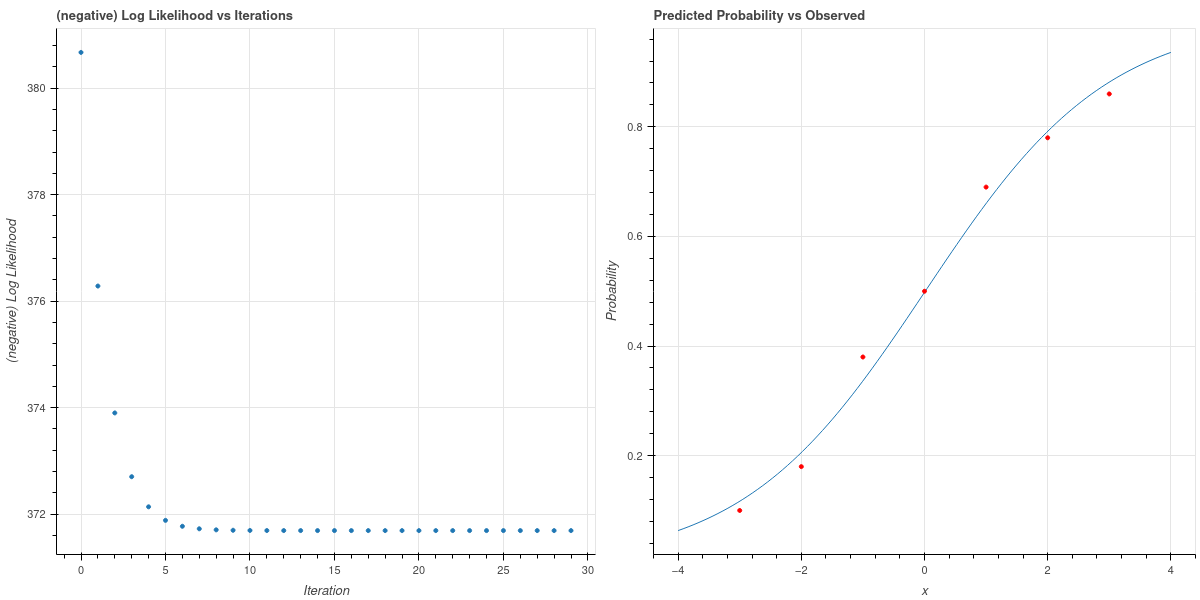
\includegraphics[width=1\textwidth,height=\textheight]{chapters/img/LogisticLogLikelihoodAndFit.png}

}

\caption{\label{fig-logisticloglike}Max Likelihood Gradient Descent for
Logistic Fitting}

\end{figure}

The parameters used to generate the data are close to this; they were
\(a=log(2)=\).6931\$ and \(b=0\).

\hypertarget{gradient-descent-and-logistic-regression-on-real-data}{%
\subsection{Gradient Descent and Logistic Regression on ``real''
data}\label{gradient-descent-and-logistic-regression-on-real-data}}

We conclude this first look at logistic regression and gradient descent
by analyzing some simple real data. This dataset consists of about
\(2200\) customers who patronize a certain food store. Among the
features in the data set is a field giving the total dollars spent at
the store by a customer; we will study that feature and its relationship
to the question of whether or not the customer accepted a special offer
from the store. (see {[}4{]} for the original data source).

\begin{figure}

{\centering 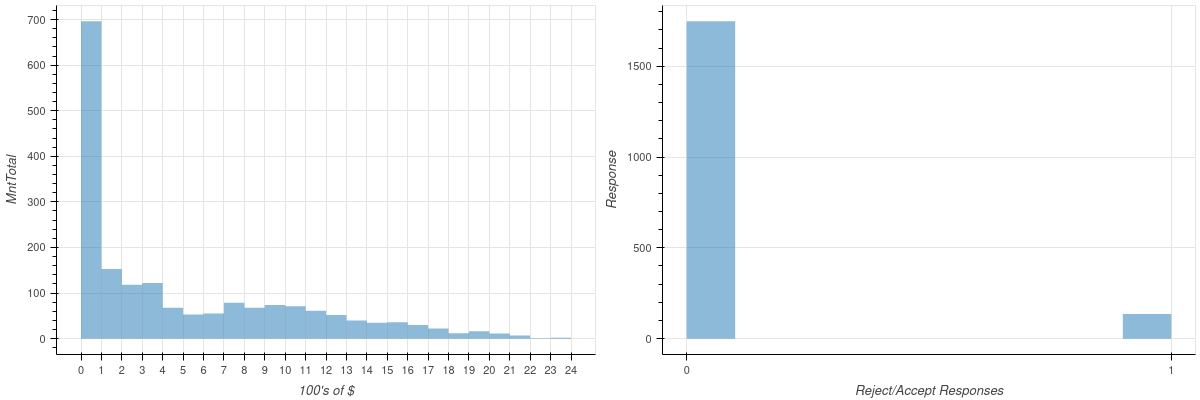
\includegraphics[width=1\textwidth,height=\textheight]{chapters/img/FoodDataPlot.png}

}

\caption{\label{fig-fooddataplot}Food Marketing Data: Histograms of
Expenditures and Response}

\end{figure}

The two plots in Figure~\ref{fig-fooddataplot} summarize the data. The
first plot is a histogram showing the amounts spent by the customers;
the second shows the distribution of responses.

We would like to know how expenditures increase the likelihood of
customers accepting our offer. We therefore fit a logistic model to the
data. The result is shown in Figure~\ref{fig-foodlogisticfit}.

\begin{figure}

{\centering 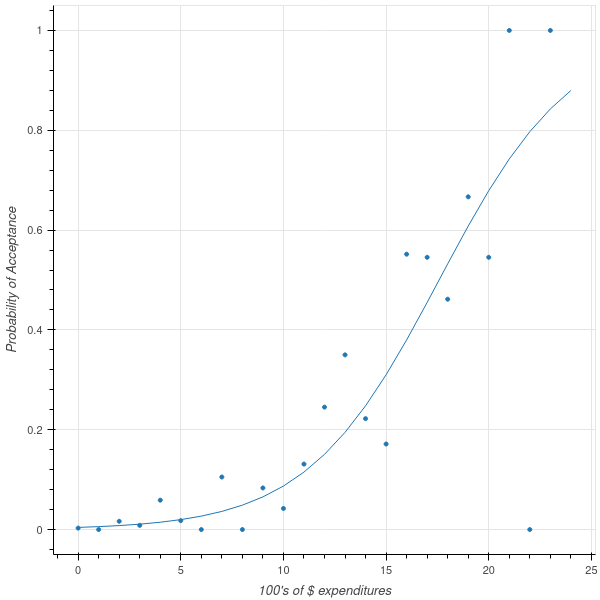
\includegraphics[width=0.5\textwidth,height=\textheight]{chapters/img/FoodLogisticFit.png}

}

\caption{\label{fig-foodlogisticfit}Logistic Model for Food Marketing}

\end{figure}

\hypertarget{logistic-regression-and-classification}{%
\section{Logistic Regression and
classification}\label{logistic-regression-and-classification}}

Beyond the kind of probability prediction that we have discussed up to
this point, logistic regression is one of the most powerful techniques
for attacking the classification problem. Let's start our discussion
with a sample problem that is a simplified version of one of the most
famous machine learning benchmark problems, the MNIST (Modified National
Institute of Science and Technology) dataset of handwritten numerals.
This dataset consists of \(60000\) labelled grayscale images of
handwritten digits from \(0\) to \(9\). Each image is stored as a
\(28x28\) array of integers from \(0\) to \(255\). Each cell of the
array corresponds to a ``pixel'' in the image, and the contents of that
cell is a grayscale value. See {[}5{]} for the a more detailed
description of how the dataset was constructed.

In Figure~\ref{fig-MNISTOne} is a picture of a handwritten ``1'' from
the MNIST dataset.

\begin{figure}

{\centering 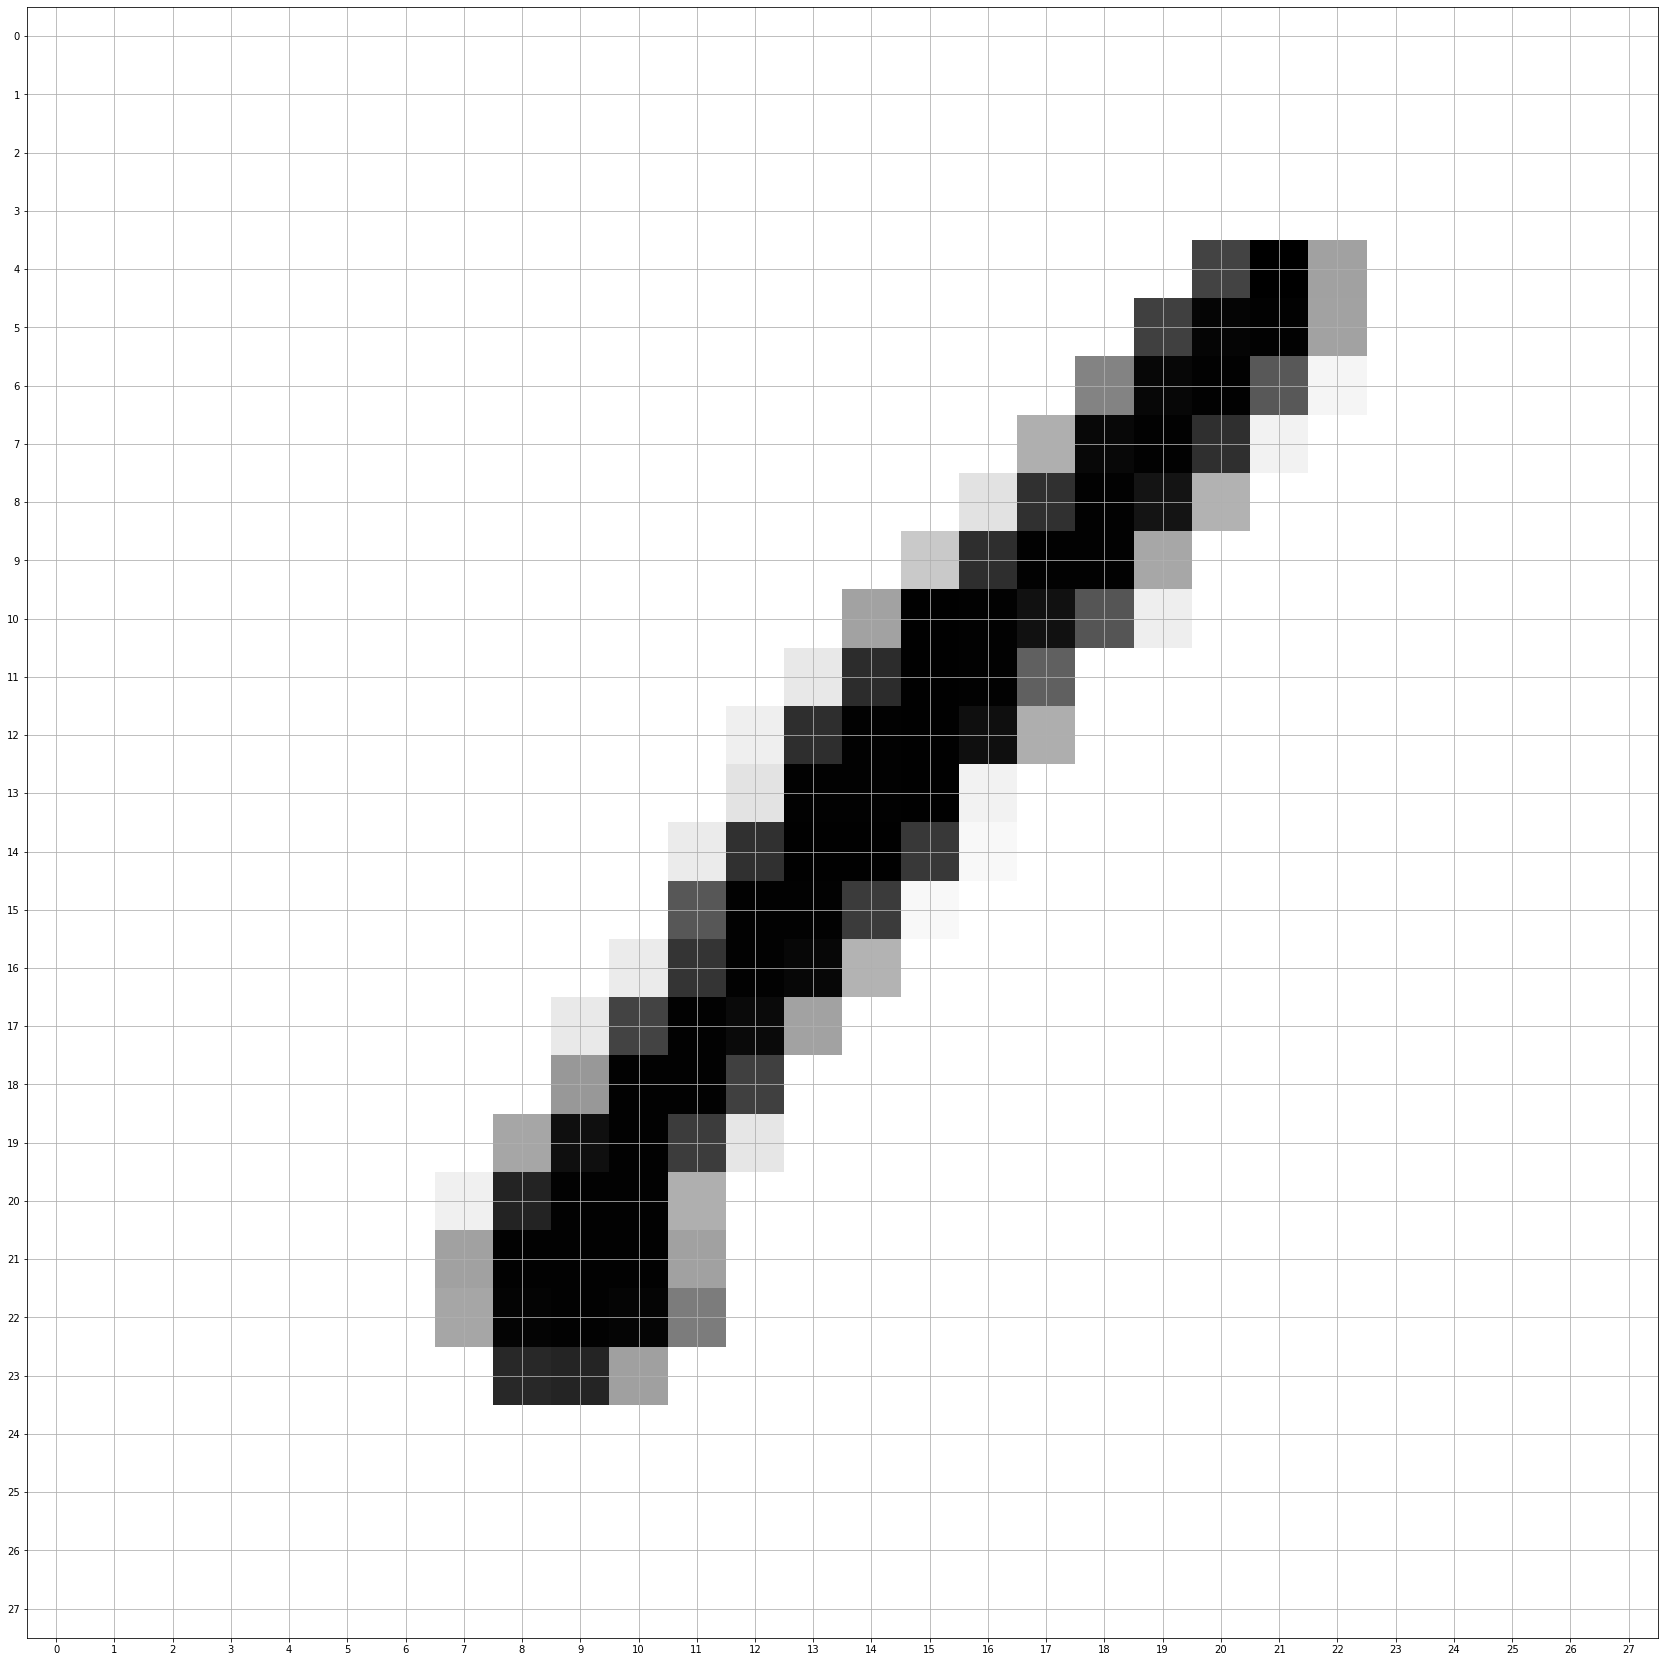
\includegraphics[width=1\textwidth,height=\textheight]{chapters/img/MNISTOne.png}

}

\caption{\label{fig-MNISTOne}Handwritten One from MNIST}

\end{figure}

\textbf{Classification Problem for MNIST:} Given a \(28x28\) array of
grayscale values, determine which digit is represented.

At first glance, this does not look like a logistic regression problem.
To make the connection clearer, let's simplify the problem and imagine
that our database contains only labelled images of zeros and ones --
we'll worry about how to handle the full problem later. So now our task
is to determine which images are zeros, and which are ones.

Our approach will be to view each image as a vector of length
\(784=28*28\) by stringing the pixel values row by row into a one
dimensional vector, which following our conventions yields a matrix of
size \(N\times 784\) where \(N\) is the number of images. Since we may
also need an ``intercept'', we add a column of \(1\)'s to our images
yielding a data matrix \(X\) of size \(N\times 785\). The labels \(y\)
form a column vector of size \(N\) containing zeros and ones.

We will also simplify the data but converting the gray-scale images to
monochrome by converting gray levels up to \(128\) as ``white'' and
beyond \(128\) as ``black''.

The logistic regression approach asks us to find the ``best'' vector
\(M\) so that, for a given image vector \(x\) (extended by adding a one
at the end), the function \[
p(x)=\frac{1}{1+e^{-xM}}
\] is close to \(1\) if \(x\) represents a one, and is close to zero if
\(x\) represents zero. Essentially we think of \(p(x)\) as giving the
probability that the vector \(x\) represents an image of a one. If we
want a definite choice, then we can set a threshold value \(p_0\) and
say that the image \(x\) is a one if \(p(x)>p_0\) and zero otherwise.
The natural choice of \(p_0=.5\) amounts to saying that we choose the
more likely of the two options under the model.

Since we are applying the logistic model we are assuming:

\begin{itemize}
\tightlist
\item
  that the value of each pixel in the image contributes something
  towards the chance of the total image being one;
\item
  and the different pixels have independent, and additive effects on the
  odds of getting a one.
\end{itemize}

If we take this point of view, then we can ask for the vector \(M\) that
is \emph{most likely} to account for the labellings, and we can use our
maximum likelihood gradient descent method to find \(M\).

This approach is surprisingly effective. With the MNIST zeros and ones,
and the gradient descent method discussed above, one can easily find
\(M\) so that the logistic model predicts the correct classification
with accuracy in the high 90\% range.

\hypertarget{weights-as-filters}{%
\subsection{Weights as filters}\label{weights-as-filters}}

One interesting aspect of using logistic regression on images for
classification is that the we can interpret the optimum set of
coefficients \(M\) as a kind of filter for our images. Remember that
\(M\) is a vector with \(785\) entries, the last of which is an
``intercept''.\\
The logistic model says that, for an image vector \(x\), the log-odds
that the image is a one is given by \[
\log \frac{p}{1-p} = \sum_{i=0}^{783} M_{i}x_{i} + M_{784}.
\] This means that if the value of \(M_{i}\) is positive, then large
values in the \(i^{th}\) pixel \emph{increase} the chance that our image
is a one; while if \(M_{i}\) is negative, large values \emph{decrease}
the chance. If \(M_{i}\) is negative, the reverse is true. However, the
values \(x_{i}\) are the gray scale ``darkness'' of the image, so the
entries of \(M\) emphasize or de-emphasize dark pixels according to
whether that dark pixel is more or less likely to occur in a one
compared to a zero.

This observation allows us to interpret the weights \(M\) as a kind of
``filter'' for the image. In fact, if we rescale the entries of \(M\)
(omitting the intercept) so that they lie between \(0\) and \(255\), we
can arrange them as a \(28\times 28\) array and plot them as an image.
The result of doing this for a selection of MNIST zeros and ones is
shown on the left in Figure~\ref{fig-weights}. The red (or positive)
weights in the middle of the image tell us that if those pixels are
dark, the image is more likely to be a one; the blue (or negative)
weights scattered farther out tell us that if those pixels are dark, the
image is more likely to be a zero.

\begin{figure}

{\centering 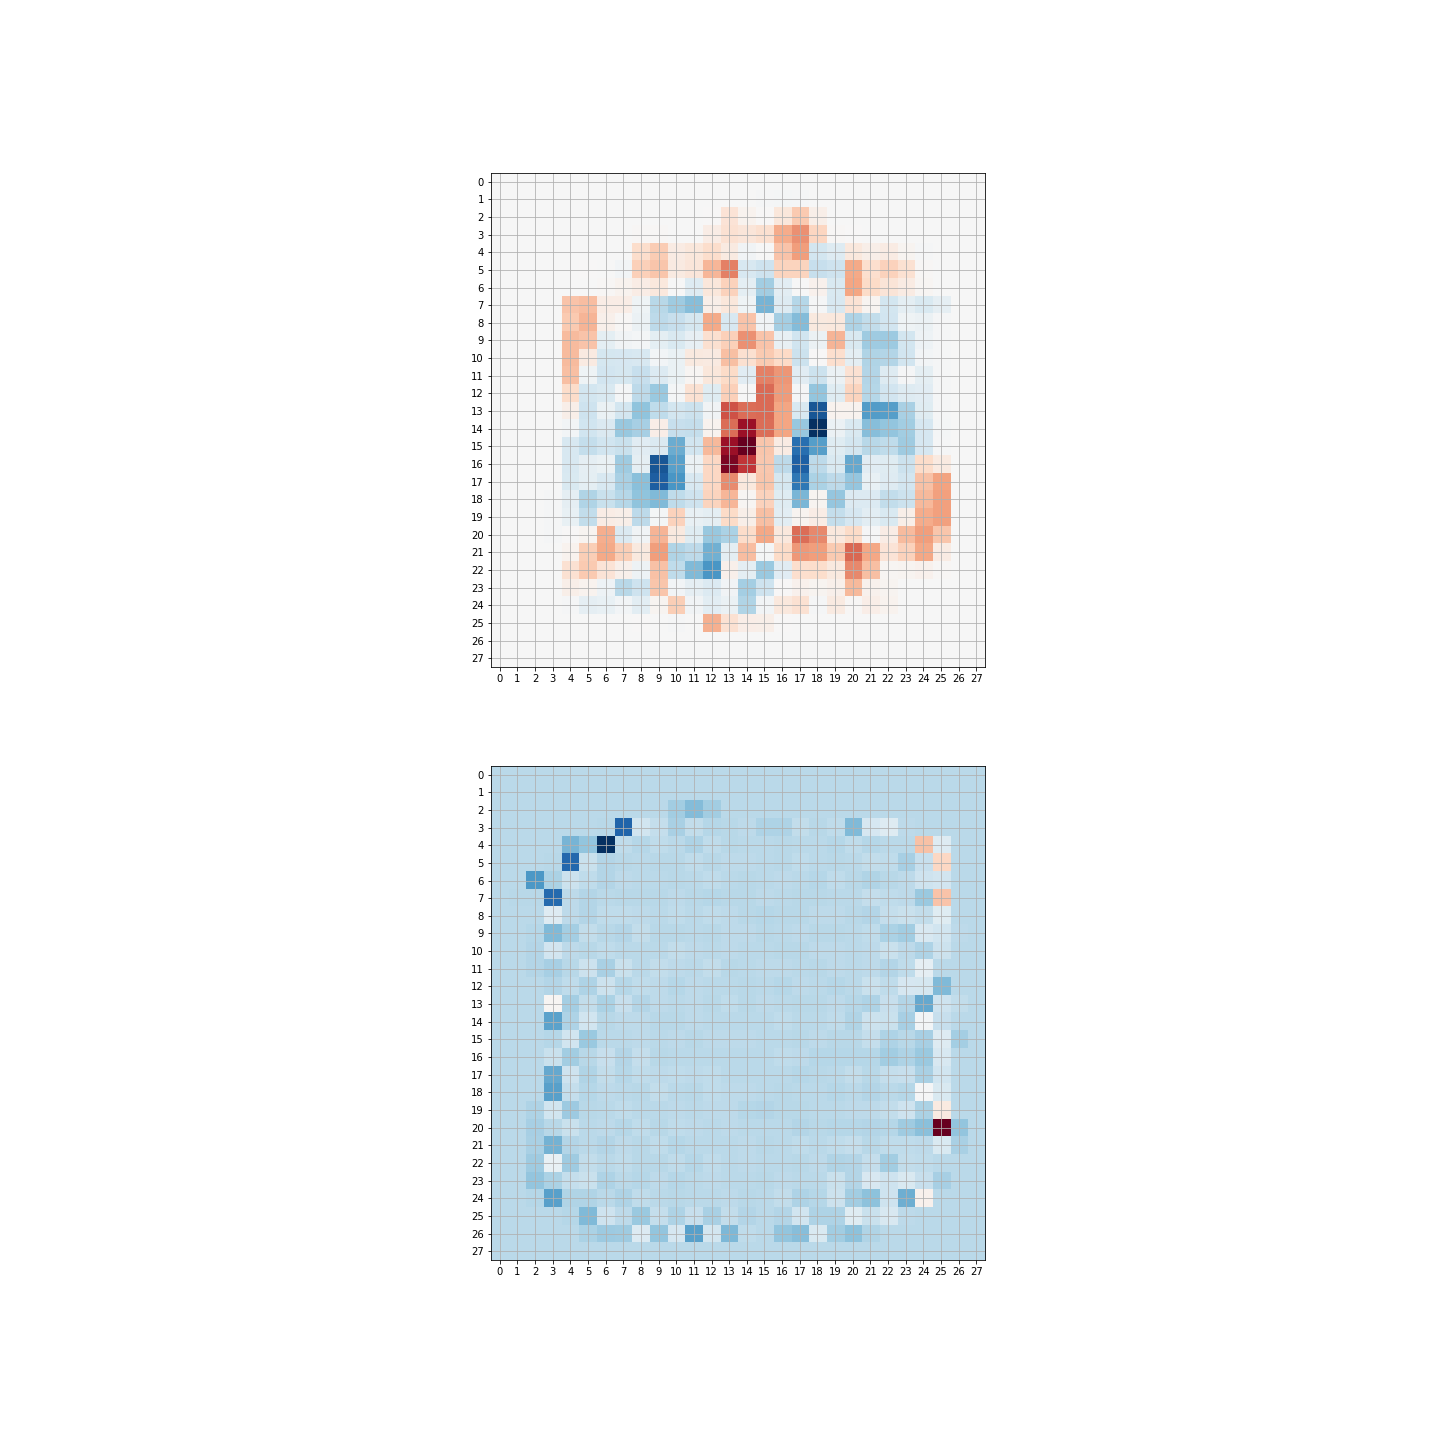
\includegraphics[width=1\textwidth,height=\textheight]{chapters/img/weights.png}

}

\caption{\label{fig-weights}Rescaled weights (blue is negative). Top: 0
vs 1. Bottom: 3 vs 8.}

\end{figure}

What's important to notice here is that we did not design this
``filter'' by hand, based on our understanding of the differences
between a handwritten zero and one; instead, the algorithm ``learned''
the ``best'' filter to optimize its ability to distinguish these digits.

Here's another example. Suppose we redo the MNIST problem above, but we
try to distinguish 3's from 8's.\\
We have about 4500 of each digit, and we label the 3's with zero and the
8's with one. Then we use our maximum likelihood optimization. In this
case, the filter is shown on the bottom in Figure~\ref{fig-weights}.

\hypertarget{multiclass-logistic-regression}{%
\section{Multiclass Logistic
Regression}\label{multiclass-logistic-regression}}

One could attack the problem of classifying the ten distinct classes of
digits by, for example, labelling all of the zeros as class zero and
everything else as class one, and finding a set of weights that
distinguishes zero from everything else. Then, in turn, one could do the
same for each of the other digits. Given an unknown image, this would
yield a set of probabilities from which one could choose the most likely
class. This type of classification is called ``one vs rest'', for
obvious reasons. It seems more natural, however, to construct a model
that, given an image, assigns a probability that it belongs to each of
the different possibilities. It is this type of multiclass logistic
regression that we will study now.

Our goal is to build a model that, given an unknown image, returns a
vector of ten probabilities, each of which we can interpret as the
chance that our unknown image is in fact of a particular digit. If we
\emph{know} the image's class, then it's probability vector
\emph{should} be nine zeros with a single one in the position
corresponding to the digit. So, for example, if our image is of a two,
then the vector of probabilities

\[
\left[ \begin{matrix} p_0 & p_1 & p_2 &\cdots & p_8 & p_9\\\end{matrix}\right]=\left[\begin{matrix} 0 &0 & 1 & \cdots & 0 & 0\\\end{matrix}\right]
\]

where \(p_i\) is the probability that our image is the digit \(i\).
Notice also that the probabilities \(p_i\) must sum to one. We encode
the class membership of our samples by constructing an \(N\times r\)
matrix \(Y\), each row of which has a one in column \(j\) if that sample
belongs to class \(j\), and zeros elsewhere. This type of representation
is sometimes called ``one-hot'' encoding.

So let's assume we have \(N\) data points, each with \(k\) features, and
a one-hot encoded, \(N\times r\) matrix of labels \(Y\) encoding the
data into \(r\) classes. As usual, we add an ``extra'' feature, which is
the constant \(1\) for each sample, to account for the ``intercept''. So
our data matrix will be \(N\times (k+1)\).

Our goal will be to find a \((k+1)\times r\) matrix of ``weights'' \(M\)
so that, for each sample, we compute \(r\) values, given by the rows of
the matrix \(XM\). These \(r\) values are linear functions of the
features, but we need probabilities. In the one-dimensional case, we
used the logistic function \(\sigma\) to convert our linear function to
probabilities. In this higher dimensional case we use a generalization
of \(\sigma\) called the ``softmax'' function.

\textbf{Definition:} Let \(F:\mathbf{R}^r\to\mathbf{R}^{r}\) be the
function \[
F(z_1,\ldots, z_r) = \sum_{j=1}^{r} e^{z_{i}}
\] and let \(\sigma:\mathbf{R}^{r}\to \mathbf{R}^{r}\) be the function
\[
\sigma(z_1,\ldots, z_n) = \left[\begin{matrix} \frac{e^{z_1}}{F} & \cdots & \frac{e^{z_{r}}}{F}\end{matrix}\right].
\] Notice that the coordinates of the vector \(\sigma(z_1,\ldots,z_n)\)
are all between \(0\) and \(1\), and their sum is one.

Our multiclass logistic model will say that the probability vector that
gives the probabilities that a particular sample belongs to a particular
class is given by the rows of the matrix \(\sigma(XM)\), where
\(\sigma(XM)\) means applying the function \(\sigma\) to each row of the
\(N\times r\) matrix \(XM\). For later computation, if:

\begin{itemize}
\tightlist
\item
  \(x=X[i,:]\) is the \(k+1\)-entry feature vector of a single sample --
  a row of the data matrix \(X\)
\item
  \(m_{j}=M[:,j]\) is the \(k+1\)-entry column vector corresponding to
  the \(j^{th}\) column of \(M\),
\end{itemize}

then the probability vector \([p_{t}]_{t=1}^{r}\) has entries \[
p_{t}(x;M) = \frac{e^{x\cdot m_{t}}}{\sum_{s=1}^{r} e^{x\cdot m_{s} }}.
\]

\hypertarget{multiclass-logistic-regression---the-likelihood}{%
\subsection{Multiclass logistic regression - the
likelihood}\label{multiclass-logistic-regression---the-likelihood}}

The probability vector \([p_{t}(x;M)]\) encodes the probabilities that
the \(x\)-value belongs to each of the possible classes. That is, \[
p_{j}(x;M)=\hbox{The chance that x is in class j}.
\]

We have captured the class membership of the samples in a
\((k+1)\times r\) matrix \(Y\) which is ``one-hot'' encoded. Each row of
this matrix has is zero in each place, except in the ``correct'' class,
where it is one. Let \(y=Y[i,:]\) be the \(i^{th}\) row of this matrix,
so it is an \(r\)-entry row vector which is \(1\) in the position giving
the ``correct'' class for our sample \(x\).

So we can represent the chance that sample \(j\) belongs to class \(i\)
as \[
P(\hbox{ sample i in class j})=\prod_{s=1}^{r} p_{s}(x;M)^{y_{s}}.
\] Taking the logarithm, we find

\begin{equation}\protect\hypertarget{eq-multiclasslikelihood}{}{
\log P = \sum_{s=1}^{r} y_{s}\log p_{s}(x;M).
}\label{eq-multiclasslikelihood}\end{equation}

Since each sample is independent, the total likelihood is the product of
these probabilites, and the log-likelihood the corresponding sum: \[
\log L(M) = \sum_{X,Y} \sum_{s=1}^{r} y_{s}\log p_{s}(x;M).
\] where the sum is over the \(N\) rows of \(X\) and \(Y\). This is
equivalent to the matrix expression \[
\log L(M) = \mathrm{trace}(Y^{\intercal}\log P)=\mathrm{trace}(Y^{\intercal}\log\sigma(XM))
\]

This is the multiclass generalization of
Equation~\ref{eq-logisticregressionlikelihood}. To see the connection,
notice that, in the case where we have only two classes, \(y_1=1-y_0\)
and \(p_{1}(x;M)=1-p_{0}(x;M)\), so this sum is the same as in the two
class situation.

\hypertarget{multiclass-logistic-regression---the-gradient.}{%
\subsection{Multiclass logistic regression - the
gradient.}\label{multiclass-logistic-regression---the-gradient.}}

To find the ``best-fitting'' multiclass logistic model by gradient
descent, we need an expression for the gradient of the likelihood
\(L(M)\). As with all of these calculations, this is an exercise in the
chain rule. We start with the formula \[
p_{s}(x;M) = \frac{e^{x\cdot m_s}}{\sum_{t=1}^{r} e^{x\cdot m_{t}}}
\] The gradient of this is made up of the derivatives with respect to
the \(m_{bq}\) where \(b=0,\ldots, k\) and \(q=1,\dots, r\) so its
natural to think of this gradient as a \((k+1)\times r\) matrix, the
same shape as \(M\). Remember that each \(m_s\) is the \(s^{th}\) column
of \(M\) so is made up of \(m_{bs}\) for \(b=0,\ldots, k\).

Looking at \[
\frac{\partial p_{s}}{\partial m_{bq}}
\] there are two cases to consider. The first is when \(q\) and \(s\)
are different, so the numerator of \(p_{s}\) doesn't involve \(m_{pq}\).
In this case the derivative is \[
\frac{\partial p_{s}}{\partial m_{bq}}=-\frac{e^{x\cdot m_{s}}e^{x\cdot m_{q}}x_b}{(\sum_{t=1}^{r} e^{x\cdot m_{t}})^2}=-p_{s}p_{q}x_{b}
\] In vector terms: \[
[\frac{\partial p_{s}}{\partial m_{bq}}]_{b=1}^{k}=-p_{q}p_{s}[x_{b}]_{b=1}^{k}
\] as an equality of \(k+1\)-entry row vectors. This can be written more
simply as a vector equation: \[
\frac{\partial p_{s}}{\partial m_{q}}=-p_{q}p_{s}x.\qquad (q\not=s).
\] When \(q=s\), we have \[
\frac{\partial p_{s}}{\partial m_{bs}}
=\frac{e^{x\cdot m_{bs}}x_b}{\sum_{t=1}^{r}e^{x\cdot m_{t}}}-\frac{e^{x\cdot m_{s}}e^{x\cdot m_{s}}x_b}{(\sum_{t=1}^{r} e^{x\cdot m_{t}})^2}=p_{s}(1-p_{s})x_b
\] or in vector terms \[
\frac{\partial p_{s}}{\partial m_{s}}=p_{s}(1-p_{s})x^{\intercal}.
\]

\textbf{Important:} The gradient on the left is properly seen as a
column vector (because \(m_{s}\) is a column of the matrix \(M\), with
\(k+1\) entries), and since \(x\) is a row of the data matrix, so to
keep the indices straight, we need \(x^{\intercal}\) on the right.

Now we can use these formulae together with the expression for
\(\log L(M)\) to obtain the gradient. Using the vector form, we have \[
\frac{\partial \log L(M)}{\partial m_{q}} = \sum_{X,Y}\sum_{s=1}^{r} y_{s}\frac{\partial \log p_{s}}{m_{q}}.
\] Using our computations above, the chain rule, and the derivative of
the logarithm, this is the sum \[
\frac{\partial \log L(M)}{\partial m_{q}} =\sum_{X,Y}\sum_{s=1}^{r} y_{s}(I_{qs}-p_{q})x^{\intercal}
\] where \(I_{qs}=1\) if \(q=s\) and zero otherwise.

Now \(y_{s}I_{qs}\) is zero unless \(s=q\), and the sum
\(\sum_{s=1}^{r} y_{s}=1\), so this simplifies further to \[
\frac{\partial \log L(M)}{\partial m_{q}} = \sum_{X,Y} (y_{q}-p_{q})x^{\intercal}.
\] This is equivalent to the matrix expression
\begin{equation}\protect\hypertarget{eq-multiclassgradient}{}{
\nabla \log L(M) = X^{\intercal}(Y-P)=X^{\intercal}(Y-\sigma(XM)).
}\label{eq-multiclassgradient}\end{equation}

Compare Equation~\ref{eq-multiclassgradient} to
Theorem~\ref{thm-logisticgradient} and we see that the form is identical
whether in the two-class or multi-class case if we set things up
properly.

\leavevmode\vadjust pre{\hypertarget{alg-graddescent}{}}%
\begin{algorithm}[Multiclass Gradient Descent]\label{alg-graddescent}

Given:

\begin{itemize}
\tightlist
\item
  an \(N\times(k+1)\) data matrix \(X\) whose last column is all \(1\),
\item
  an \(N\times r\) matrix \(Y\) that ``one-hot'' encodes the labels of
  the classification problem;
\item
  a random \((k+1)\times r\) matrix \(M\) of initial guesses for the
  parameters
\item
  a ``learning rate'' \(\nu\),
\end{itemize}

Iterate: \[
M^{(j+1)}=M^{(j)}+\nu X^{\intercal}(Y-\sigma(XM^{(j)}))
\] until \(M\) changes by less than some tolerance.

\end{algorithm}

\hypertarget{stochastic-gradient-descent-for-logistic-regression}{%
\section{Stochastic Gradient Descent for Logistic
Regression}\label{stochastic-gradient-descent-for-logistic-regression}}

The gradient descent process for logistic regression suffers from the
same limitation as for linear regression that we discussed in
\textbf{?@sec-sgd}. Each iteration requires us to compute the matrix
product \(X^{\intercal}(Y-\sigma(XM^{(j)}))\) which uses all of the data
and is therefore time- and even more importantly memory-intensive.

Therefore logistic regression is also a candidate for stochastic
gradient descent, in which we iterate over each data point \(x\) and
associated target \(y\) and make adjustments point by point. To do this
we use the gradient from Equation~\ref{eq-multiclassgradient} in the
much simpler case where \(X\) is a single row of the data matrix and
\(Y\) is a row vector that is zero except for a one in the spot
corresponding to the target class for \(X\).

\bookmarksetup{startatroot}

\hypertarget{support-vector-machines}{%
\chapter{Support Vector Machines}\label{support-vector-machines}}

\hypertarget{introduction-4}{%
\section{Introduction}\label{introduction-4}}

Suppose that we are given a collection of data made up of samples from
two different classes, and we would like to develop an algorithm that
can distinguish between the two classes. For example, given a picture
that is either a dog or a cat, we'd like to be able to say which of the
pictures are dogs, and which are cats. For another example, we might
want to be able to distinguish ``real'' emails from ``spam.'' This type
of problem is called a \emph{classification} problem.

Typically, one approaches a classification problem by beginning with a
large set of data for which you know the classes, and you use that data
to \emph{train} an algorithm to correctly distinguish the classes for
the test cases where you already know the answer. For example, you start
with a few thousand pictures labelled ``dog'' and ``cat'' and you build
your algorithm so that it does a good job distinguishing the dogs from
the cats in this initial set of \emph{training data}. Then you apply
your algorithm to pictures that aren't labelled and rely on the
predictions you get, hoping that whatever let your algorithm distinguish
between the particular examples will generalize to allow it to correctly
classify images that aren't pre-labelled.

Because classification is such a central problem, there are many
approaches to it. We will see several of them through the course of
these lectures. We will begin with a particular classification algorithm
called ``Support Vector Machines'' (SVM) that is based on linear
algebra. The SVM algorithm is widely used in practice and has a
beautiful geometric interpretation, so it will serve as a good beginning
for later discussion of more complicated classification algorithms.

Incidentally, I'm not sure why this algorithm is called a ``machine'';
the algorithm was introduced in the paper {[}6{]} where it is called the
``Optimal Margin Classifier'' and as we shall see that is a much better
name for it.

My presentation of this material was heavily influenced by the beautiful
paper {[}7{]}.

\hypertarget{a-simple-example}{%
\section{A simple example}\label{a-simple-example}}

Let us begin our discussion with a very simple dataset (see {[}8{]} and
{[}9{]}). This data consists of various measurements of physical
characteristics of 344 penguins of 3 different species: Gentoo, Adelie,
and Chinstrap. If we focus our attention for the moment on the Adelie
and Gentoo species, and plot their body mass against their culmen depth,
we obtain the following scatterplot.

\begin{figure}

{\centering 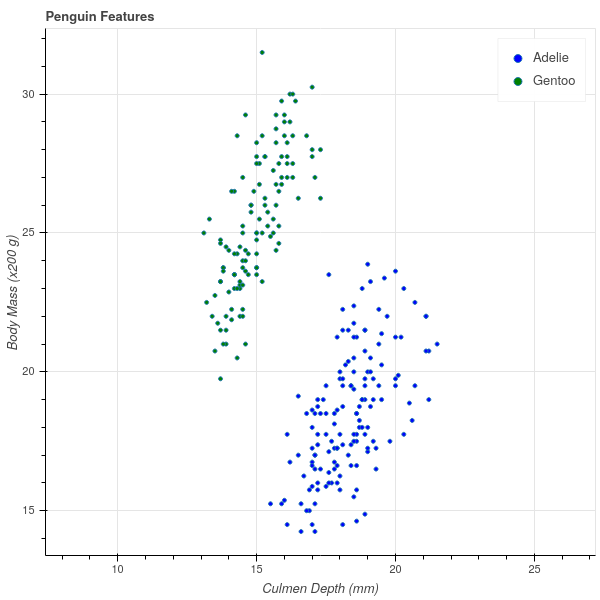
\includegraphics[width=0.5\textwidth,height=\textheight]{chapters/img/penguins.png}

}

\caption{\label{fig-penguins}Penguin Scatterplot}

\end{figure}

Incidentally, a bird's \emph{culmen} is the upper ridge of their beak,
and the \emph{culmen depth} is a measure of the thickness of the beak.
There's a nice picture at {[}9{]} for the penguin enthusiasts.

A striking feature of this scatter plot is that there is a clear
separation between the clusters of Adelie and Gentoo penguins. Adelie
penguins have deeper culmens and less body mass than Gentoo penguins.
These characteristics seem like they should provide a way to classify a
penguin between these two species based on these two measurements.

One way to express the separation between these two clusters is to
observe that one can draw a line on the graph with the property that all
of the Adelie penguins lie on one side of that line and all of the
Gentoo penguins lie on the other. In Figure~\ref{fig-penguinsline} I've
drawn in such a line (which I found by eyeballing the picture in
Figure~\ref{fig-penguins}). The line has the equation \[
Y = 1.25X+2.
\]

\begin{figure}

{\centering 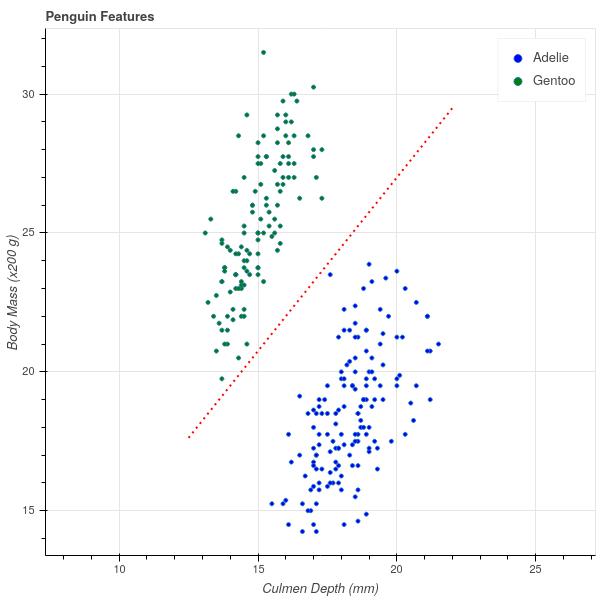
\includegraphics[width=0.5\textwidth,height=\textheight]{chapters/img/penguins_with_line.png}

}

\caption{\label{fig-penguinsline}Penguins with Separating Line}

\end{figure}

The fact that all of the Gentoo penguins lie above this line means that,
for the Gentoo penguins, their body mass in grams is at least \(400\)
more than \(250\) times their culmen depth in mm. (Note that the \(y\)
axis of the graph is scaled by \(200\) grams).

\[
\mathrm{Gentoo\ mass}> 250(\mathrm{Gentoo\ culmen\ depth})+400
\]

while

\[
\mathrm{Adelie\ mass}<250(\mathrm{Adelie\ culmen\ depth})+400.
\]

Now, if we measure a penguin caught in the wild, we can compute
\(250(\mathrm{culmen\ depth})+400\) for that penguin and if this number
is greater than the penguin's mass, we say it's an Adelie; otherwise, a
Gentoo. Based on the experimental data we've collected -- the
\emph{training} data -- this seems likely to work pretty well.

\hypertarget{the-general-case}{%
\section{The general case}\label{the-general-case}}

To generalize this approach, let's imagine now that we have \(n\)
samples and \(k\) features (or measurements) for each sample. As before,
we can represent this data as an \(n\times k\) data matrix \(X\). In the
penguin example, our data matrix would be \(344\times 2\), with one row
for each penguin and the columns representing the mass and the culmen
depth. In addition to this numerical data, we have a classification that
assigns each row to one of two classes. Let's represent the classes by a
\(n\times 1\) vector \(Y\), where \(y_{i}=+1\) if the \(i^{th}\) sample
is in one class, and \(y_{i}=-1\) if that \(i^{th}\) sample is in the
other. Our goal is to predict \(Y\) based on \(X\) -- but unlike in
linear regression, \(Y\) takes on the values of \(\pm 1\).

In the penguin case, we were able to find a line that separated the two
classes and then classify points by which side of the line the point was
on. We can generalize this notion to higher dimensions. Before attacking
that generalization, let's recall a few facts about the generalization
to \(\mathbf{R}^{k}\) of the idea of a line.

\hypertarget{hyperplanes}{%
\subsection{Hyperplanes}\label{hyperplanes}}

The correct generalization of a line given by an equation
\(w_1 x_1+ w_2 w_2+b=0\) in \(\mathbf{R}^{2}\) is an equation \(f(x)=0\)
where \(f(x)\) is a degree one polynomial
\begin{equation}\protect\hypertarget{eq-degreeone}{}{
f(x) = f(x_1,\ldots, x_k) = w_1 x_1 + w_2 x_2 +\cdots + w_k x_k + b 
}\label{eq-degreeone}\end{equation}

It's easier to understand the geometry of an equation like \(f(x)=0\) in
Equation~\ref{eq-degreeone} if we think of the coefficients \(w_i\) as
forming a \emph{nonzero} vector \(w = (w_1,\ldots, w_k)\) in
\(\mathbf{R}^{k}\) and writing the formula for \(f(x)\) as \[
f(x) = w\cdot x +b
\].

\textbf{Lemma:} Let \(f(x)=w\cdot x+b\) with \(w\in\mathbf{R}^{k}\) a
nonzero vector and \(b\) a constant in \(\mathbf{R}\).

\begin{itemize}
\tightlist
\item
  The inequalities \(f(x)>0\) and \(f(x)<0\) divide up
  \(\mathbf{R}^{k}\) into two disjoint subsets (called half spaces), in
  the way that a line in \(\mathbf{R}^{2}\) divides the plane in half.
\item
  The vector \(w\) is normal vector to the hyperplane \(f(x)=0\).
  Concretely this means that if \(p\) and \(q\) are any two points in
  that hyperplane, then \(w\cdot (p-q)=0\).
\item
  Let \(p=(u_1,\ldots,u_k)\) be a point in \(\mathbf{R}^{k}\). Then the
  perpendicular distance \(D\) from \(p\) to the hyperplane \(f(x)=0\)
  is \[
  D = \frac{f(p)}{\|w\|}
  \]
\end{itemize}

\textbf{Proof:} The first part is clear since the inequalities are
mutually exclusive. For the secon part, suppose that \(p\) and \(q\)
satisfy \(f(x)=0\). Then \(w\cdot p+b = w\cdot q+b=0\). Subtracting
these two equations gives \(w\cdot (p-q)=0\), so \(p-q\) is orthogonal
to \(w\).

For the third part, consider Figure~\ref{fig-triangle}. The point \(q\)
is an arbitrary point on the hyperplane defined by the equation
\(w\cdot x+b=0\). The distance from the hyperplane to \(p\) is measured
along the dotted line perpendicular to the hyperplane. The dot product
\(w\cdot (p-q) = \|w\|\|p-q\|\cos(\theta)\) where \(\theta\) is the
angle between \(p-q\) and \(w\) -- which is complementary to the angle
between \(p-q\) and the hyperplane. The distance \(D\) is therefore \[
D=\frac{w\cdot(p-q)}{\|w\|}.
\] However, since \(q\) lies on the hyperplane, we know that
\(w\cdot q+b=0\) so \(w\cdot q = -b\). Therefore
\(w\cdot(p-q)=w\cdot p+b=f(p)\), which is the formula we seek.

\begin{figure}

{\centering 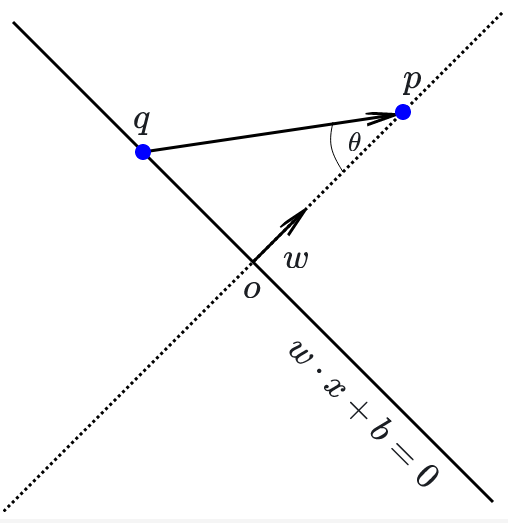
\includegraphics[width=0.3\textwidth,height=\textheight]{chapters/img/triangle.png}

}

\caption{\label{fig-triangle}Distance to a Hyperplane}

\end{figure}

\hypertarget{sec-linearseparable}{%
\subsection{Linear separability and Margins}\label{sec-linearseparable}}

Now we can return to our classification scheme. The following definition
generalizes our two dimensional picture from the penguin data.

\textbf{Definition:} Suppose that we have an \(n\times k\) data matrix
\(X\) and a set of labels \(Y\) that assign the \(n\) samples to one of
two classes. Then the labelled data is said to be \emph{linearly
separable} if there is a vector \(w\) and a constant \(b\) so that, if
\(f(x)=w\cdot x+b\), then \(f(x)>0\) whenever \(x=(x_1,\ldots, x_k)\) is
a row of \(X\) -- a sample -- belonging to the \(+1\) class, and
\(f(x)<0\) whenever \(x\) belongs to the \(-1\) class. The solutions to
the equation \(f(x)=0\) in this situation form a hyperplane that is
called a \emph{separating hyperplane} for the data.

In the situation where our data falls into two classes that are linearly
separable, our classification strategy is to find a separating
hyperplane \(f\) for our training data. Then, given a point \(x\) whose
class we don't know, we can evaluate \(f(x)\) and assign \(x\) to a
class depending on whether \(f(x)>0\) or \(f(x)<0\).

This definition begs two questions about a particular dataset:

\begin{enumerate}
\def\labelenumi{\arabic{enumi}.}
\tightlist
\item
  How do we tell if the two classes are linearly separable?
\item
  If the two sets are linearly separable, there are infinitely many
  separating hyperplanes. To see this, look back at the penguin example
  and notice that we can `wiggle' the red line a little bit and it will
  still separate the two sets. Which is the `best' separating
  hyperplane?
\end{enumerate}

Let's try to make the first of these two questions concrete. We have two
sets of points \(A\) and \(B\) in \(\mathbf{R}^{k}\), and we want to
(try to) find a vector \(w\) and a constant \(b\) so that
\(f(x)=w\cdot x+b\) takes strictly positive values for \(x\in A\) and
strictly negative ones for \(x\in B\). Let's approach the problem by
first choosing \(w\) and then asking whether there is a \(b\) that will
work. In the two dimensional case, this is equivalent to choosing the
slope of our line, and then asking if we can find an intercept so that
the line passes between the two classes.

In algebraic terms, we are trying to solve the following system of
inequalities: given \(w\), find \(b\) so that: \[
w\cdot x+b>0 \hbox{ for all $x$ in A}
\] and \[
w\cdot x+b<0\hbox{ for all $x$ in B}.
\] This is only going to be possible if there is a gap between the
smallest value of \(w\cdot x\) for \(x\in A\) and the largest value of
\(w\cdot x\) for \(x\in B\). In other words, given \(w\) there is a
\(b\) so that \(f(x)=w\cdot x+b\) separates \(A\) and \(B\) if \[
\max_{x\in B}w\cdot x < \min_{x\in A} w\cdot x.
\] If this holds, then choose \(b\) so that \(-b\) lies in this open
interval and you will obtain a separating hyperplane.

\textbf{Proposition:} The sets \(A\) and \(B\) are linearly separable if
there is a \(w\) so that \[
\max_{x\in B}w\cdot x < \min_{x\in A} w\cdot x
\] If this inequality holds for some \(w\), and \(-b\) within this open
interval, then \(f(x)=w\cdot x+b\) is a separating hyperplane for \(A\)
and \(B\).

*Figure~\ref{fig-penguinhwy2} is an illustration of this argument for a
subset of the penguin data. Here, we have fixed \(w=(1.25,-1)\) coming
from the line \(y=1.25x+2\) that we eyeballed earlier. For each Gentoo
(green) point \(x_{i}\), we computed \(-b=w\cdot x_{i}\) and drew the
line \(f(x) = w\cdot x - w\cdot x_{i}\) giving a family of parallel
lines through each of the green points. Similarly for each Adelie (blue)
point we drew the corresponding line. The maximum value of \(w\cdot x\)
for the blue points turned out to be \(1.998\) and the minimum value of
\(w\cdot x\) for the green points turned out to be \(2.003\). Thus we
have two lines with a gap between them, and any parallel line in that
gap will separate the two sets.

Finally, among all the lines \emph{with this particular \(w\)}, it seems
that the \textbf{best} separating line is the one running right down the
middle of the gap between the boundary lines. Any other line in the gap
will be closer to either the blue or green set that the midpoint line
is.

\begin{figure}

{\centering 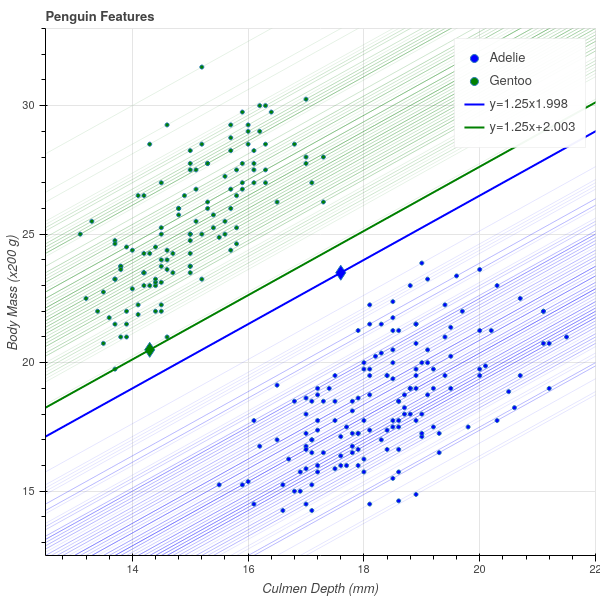
\includegraphics[width=0.5\textwidth,height=\textheight]{chapters/img/penguinhwy2.png}

}

\caption{\label{fig-penguinhwy2}Lines in Penguin Data for
\(w=(1.25,-1)\)}

\end{figure}

Let's put all of this together and see if we can make sense of it in
general.

Suppose that \(A^{+}\) and \(A^{-}\) are finite point sets in
\(\mathbf{R}^{k}\) and \(w\in\mathbf{R}^{k}\) such that \[
B^{-}(w)=\max_{x\in A^{-}}w\cdot x < \min_{x\in A^{+}}w\cdot x=B^{+}(w).
\] Let \(x^{-}\) be a point in \(A^{-}\) with \(w\cdot x^{-}=B^{-}(w)\)
and \(x^{+}\) be a point in \(A\) with \(w\cdot x^{+}=B^{+}(w)\). The
two hyperplanes \(f^{\pm}(x) = w\cdot x - B^{\pm}\) have the property
that: \[
f^{+}(x)\ge 0\hbox{ for }x\in A^{+}\hbox{ and }f^{+}(x)<0\hbox{ for }x\in A^{-}
\] and \[
f^{-}(x)\le 0\hbox{ for }x\in A^{-}\hbox{ and }f^{-}(x)>0\hbox{ for }x\in A^{+}
\]

Hyperplanes like \(f^{+}\) and \(f^{-}\), which ``just touch'' a set of
points, are called supporting hyperplanes.

\textbf{Definition:} Let \(A\) be a set of points in \(\mathbf{R}^{k}\).
A hyperplane \(f(x)=w\cdot x+b=0\) is called a \emph{supporting
hyperplane} for \(A\) if \(f(x)\ge 0\) for all \(x\in A\) and \(f(x)=0\)
for at least one point in \(A\), or if \(f(x)\le 0\) for all \(x\in A\)
and \(f(x)=0\) for at least one point in \(A\).

The gap between the two supporting hyperplanes \(f^{+}\) and \(f^{-}\)
is called the \emph{margin} between \(A\) and \(B\) for \(w\).

\textbf{Definition:} Let \(f^{+}\) and \(f^{-}\) be as in the discussion
above for point sets \(A^{+}\) and \(A^{-}\) and vector \(w\). Then the
orthogonal distance between the two hyperplanes \(f^{+}\) and \(f^{-}\)
is called the geometric margin \(\tau_{w}(A^{+},A^{-})\) (along \(w\))
between \(A^{+}\) and \(A^{-}\). We have \[
\tau_{w}(A^{+},A^{-})=\frac{B^{+}(w)-B^{-}(w)}{\|w\|}.
\]

Now we can propose an answer to our second question about the best
classifying hyperplane.

\textbf{Definition:} The \emph{optimal margin} \(\tau(A^{+},A^{-})\)
between \(A^{+}\) and \(A^{-}\) is the largest value of \(\tau_{w}\)
over all possible \(w\) for which \(B^{-}(w)<B^{+}(w)\): \[
\tau(A^{+},A^{-}) = \max_{w} \tau_{w}(A^{+},A^{-}).
\] If \(w\) is such that \(\tau_{w}=\tau\), then the hyperplane
\(f(x)=w\cdot x - \frac{(B^{+}+B^{-})}{2}\) is the \emph{optimal margin
classifying hyperplane}.

The optimal classifying hyperplane runs ``down the middle'' of the gap
between the two supporting hyperplanes \(f^{+}\) and \(f^{-}\) that give
the sides of the optimal margin.

We can make one more observation about the maximal margin. If we find a
vector \(w\) so that \(f^{+}(x) = w\cdot x -B^{+}\) and
\(f^{-}(x) = w\cdot x-B^{-}\) are the two supporting hyperplanes such
that the gap between them is the optimal margin, then this gap gives us
an estimate on how close together the points in \(A^{+}\) and \(A^{-}\)
can be. This is visible in Figure~\ref{fig-penguinhwy2}, where it's
clear that to get from a blue point to a green one, you have to cross
the gap between the two supporting hyperplanes.

\textbf{Proposition:} The closest distance between points in \(A^{+}\)
and \(A^{-}\) is greater than or equal to the optimal margin: \[
\min_{p\in A^{+},q\in A^{-}} \|p-q\|\ge \tau(A^{+},A^{-})
\].

\textbf{Proof:} We have \(f^{+}(p) = w\cdot p - B^{+}\ge 0\) and
\(f^{-}(q) = w\cdot q -B^{-}\le 0\). These two inequalities imply that
\[
w\cdot (p-q)\ge B^{+}-B^{-}>0.
\] Therefore \[
\|p-q\|\|w\|\ge |w\cdot (p-q)|\ge |B^{+}-B^{-}|
\] and so \[
\|p-q\| \ge \frac{B^{+}-B^{-}}{\|w\|} = \tau(A^{+},A^{-})
\]

If this inequality were always \emph{strict} -- that is, if the optimal
margin equalled the minimum distance between points in the two clusters
-- then this would give us an approach to finding this optimal margin.

Unfortunately, that isn't the case. In Figure~\ref{fig-nonstrict}, we
show a very simple case involving only six points in total in which the
distance between the closest points in \(A^{+}\) and \(A^{-}\) is larger
than the optimal margin.

\begin{figure}

{\centering 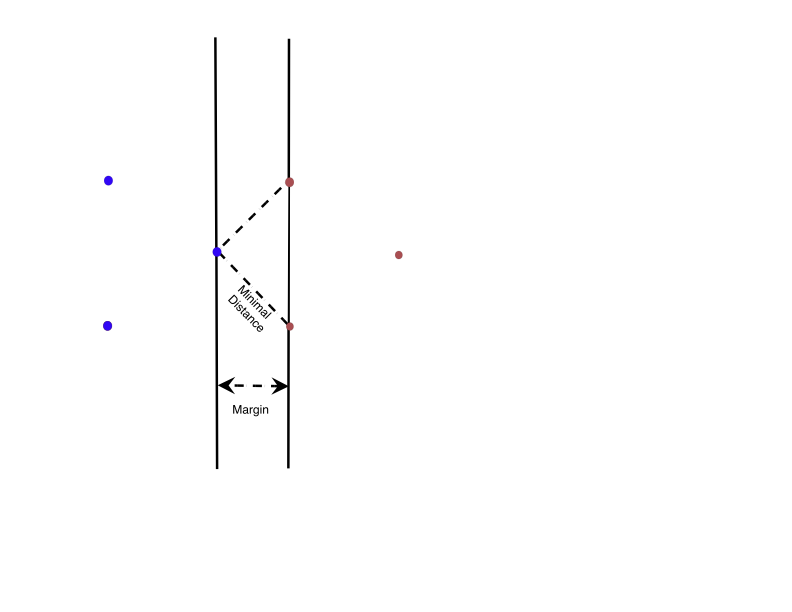
\includegraphics[width=\textwidth,height=3in]{chapters/img/margindistance2.png}

}

\caption{\label{fig-nonstrict}Shortest distance between + and - points
can be greater than the optimal margin}

\end{figure}

At least now our problem is clear. Given our two point sets \(A^{+}\)
and \(A^{-}\), find \(w\) so that \(\tau_{w}(A^{+},A^{-})\) is maximal
among all \(w\) where \(B^{-}(w)<B^{+}(w)\). This is an optimization
problem, but unlike the optimization problems that arose in our
discussions of linear regression and principal component analysis, it
does not have a closed form solution. We will need to find an algorithm
to determine \(w\) by successive approximations. Developing that
algorithm will require thinking about a new concept known as
\emph{convexity.}

\hypertarget{convexity-convex-hulls-and-margins}{%
\section{Convexity, Convex Hulls, and
Margins}\label{convexity-convex-hulls-and-margins}}

In this section we introduce the notion of a \emph{convex set} and the
particular case of the \emph{convex hull} of a finite set of points. As
we will see, these ideas will give us a different interpretation of the
margin between two sets and will eventually lead to an algorithm for
finding the optimal margin classifier.

\textbf{Definition:} A subset \(U\) of \(\mathbf{R}^{k}\) is
\emph{convex} if, for any pair of points \(p\) and \(q\) in \(U\), every
point \(t\) on the line segment joining \(p\) and \(q\) also belongs to
\(U\). In vector form, for every \(0\le s\le 1\), the point
\(t(s) = (1-s)p+sq\) belongs to \(U\). (Note that \(t(0)=p\),
\(t(1)=q\), and so \(t(s)\) traces out the segment joining \(p\) to
\(q\).)

*Figure~\ref{fig-convexnotconvex} illustrates the difference between
convex sets and non-convex ones.

\begin{figure}

{\centering 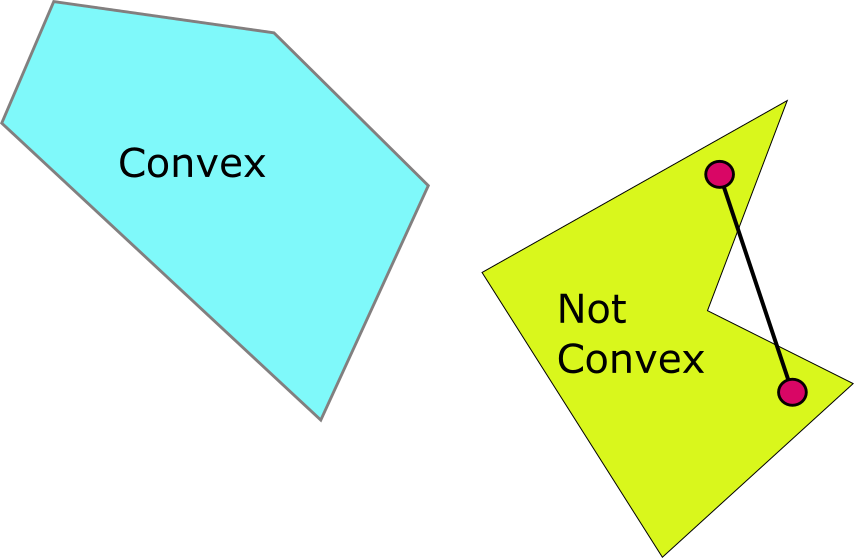
\includegraphics[width=\textwidth,height=3in]{chapters/img/ConvexNotConvex.png}

}

\caption{\label{fig-convexnotconvex}Convex vs Non-Convex Sets}

\end{figure}

The key idea from convexity that we will need to solve our optimization
problem and find the optimal margin is the idea of the \emph{convex
hull} of a finite set of points in \(\mathbf{R}^{k}\).

\textbf{Definition:} Let \(S=\{q_1,\ldots, q_{N}\}\) be a finite set of
\(N\) points in \(\mathbf{R}^{k}\). The \emph{convex hull} \(C(S)\) of
\(S\) is the set of points \[
p = \sum_{i=1}^{N} \lambda_{i}q_{i}
\] as \(\lambda_{1},\ldots,\lambda_{N}\) runs over all positive real
numbers such that \[
\sum_{i=1}^{N} \lambda_{i} = 1.
\]

There are a variety of ways to think about the convex hull \(C(S)\) of a
set of points \(S\), but perhaps the most useful is that it is the
smallest convex set that contains all of the points of \(S\). That is
the content of the next lemma.

\textbf{Lemma:} \(C(S)\) is convex. Furthermore, let \(U\) be any convex
set containing all of the points of \(S\). Then \(U\) contains \(C(S)\).

\textbf{Proof:} To show that \(C(S)\) is convex, we apply the
definition. Let \(p_1\) and \(p_2\) be two points in \(C(S)\), so that
let \(p_{j}=\sum_{i=1}^{N} \lambda^{(j)}_{i}q_{i}\) where
\(\sum_{i=1}^{N}\lambda^{(j)}_{i} = 1\) for \(j=1,2\). Then a little
algebra shows that \[
(1-s)p_1+sp_{2} = \sum_{i=1}^{N} (s\lambda^{(1)}_{i}+(1-s)\lambda^{(2)}_{i})q_{i}
\] and
\(\sum_{i=1}^{N} (s\lambda^{(1)}_{i}+(1-s)\lambda^{(2)}_{i}) = 1\).
Therefore all of the points \((1-s)p_{1}+sp_{2}\) belong to \(C(S)\),
and therefore \(C(S)\) is convex.

For the second part, we proceed by induction. Let \(U\) be a convex set
containing \(S\). Then by the definition of convexity, \(U\) contains
all sums \(\lambda_{i}q_{i}+\lambda_{j}q_{j}\) where
\(\lambda_i+\lambda_j=1\). Now suppose that \(U\) contains all the sums
\(\sum_{i=1}^{N} \lambda_{i}q_{i}\) where exactly \(m-1\) of the
\(\lambda_{i}\) are non-zero for some \(m<N\).\\
Consider a sum \[
q = \sum_{i=1}^{N}\lambda_{i}q_{i}
\] with exactly \(m\) of the \(\lambda_{i}\not=0\). For simplicity let's
assume that \(\lambda_{i}\not=0\) for \(i=1,\ldots, m\). Now let
\(T=\sum_{i=1}^{m-1}\lambda_{i}\) and set \[
q' = \sum_{i=1}^{m-1}\frac{\lambda_{i}}{T}q_{i}.
\] This point \(q'\) belongs to \(U\) by the inductive hypothesis. Also,
\((1-T)=\lambda_{m}\). Therefore by convexity of \(U\), \[
q = (1-T)q_{m}+Tq'
\] also belongs to \(U\). It follows that all of \(C(S)\) belongs to
\(U\).

In Figure~\ref{fig-convexhull} we show our penguin data together with
the convex hull of points corresponding to the two types of penguins.
Notice that the boundary of each convex hull is a finite collection of
line segments that join the ``outermost'' points in the point set.

\begin{figure}

{\centering 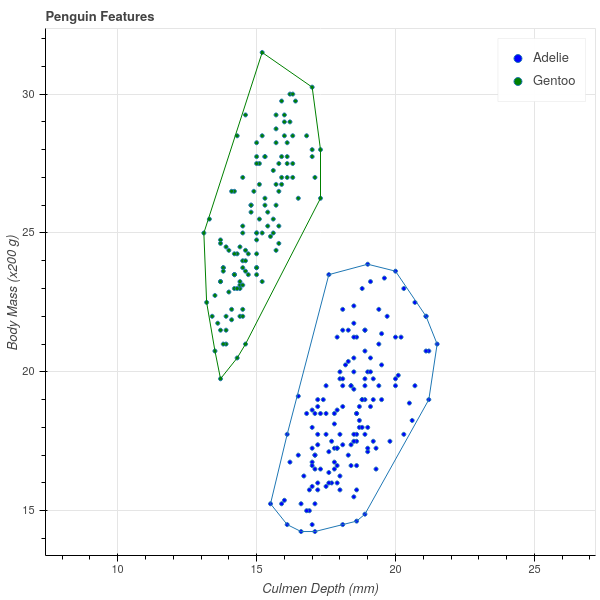
\includegraphics[width=0.5\textwidth,height=\textheight]{chapters/img/penguinswithhulls.png}

}

\caption{\label{fig-convexhull}The Convex Hull}

\end{figure}

One very simple example of a convex set is a half-plane. More
specifically, if \(f(x)=w\cdot x+b=0\) is a hyperplane, then the two
``sides'' of the hyperplane, meaning the subsets \(\{x: f(x)\ge 0\}\)
and \(\{x: f(x)\le 0\}\), are both convex. (This is exercise 1 in
Section~\ref{sec-exercises} ).

As a result of this observation, and the Lemma above, we can conclude
that if \(f(x)=w\cdot x+b=0\) is a supporting hyperplane for the set
\(S\) -- meaning that either \(f(x)\ge 0\) for all \(x\in S\), or
\(f(x)\le 0\) for all \(x\in S\), with at least one point \(x\in S\)
such that \(f(x)=0\) -- then \(f(x)=0\) is a supporting hyperplane for
the entire convex hull. After all, if \(f(x)\ge 0\) for all points
\(x\in S\), then \(S\) is contained in the convex set of points where
\(f(x)\ge 0\), and therefore \(C(S)\) is contained in that set as well.

Interestingly, however, the converse is true as well -- the supporting
hyperplanes of \(C(S)\) are exactly the same as those for \(S\).

\textbf{Lemma:} Let \(S\) be a finite set of points in
\(\mathbf{R}^{k}\) and let \(f(x)=w\cdot x +b=0\) be a supporting
hyperplane for \(C(S)\). Then \(f(x)\) is a supporting hyperplane for
\(S\).

\textbf{Proof:} Suppose \(f(x)=0\) is a supporting hyperplane for
\(C(S)\). Let's assume that \(f(x)\ge 0\) for all \(x\in C(S)\) and
\(f(x^{*})=0\) for a point \(x^{*}\in C(S)\), since the case where
\(f(x)\le 0\) is identical. Since \(S\subset C(S)\), we have
\(f(x)\ge 0\) for all \(x\in S\). To show that \(f(x)=0\) is a
supporting hyperplane, we need to know that \(f(x)=0\) for at least one
point \(x\in S\).\\
Let \(x'\) be the point in \(S\) where \(f(x')\) is minimal among all
\(x\in S\). Note that \(f(x')\ge 0\). Then the hyperplane
\(g(x) = f(x)-f(x')\) has the property that \(g(x)\ge 0\) on all of
\(S\), and \(g(x')=0\). Since the halfplane \(g(x)\ge 0\) is convex and
contains all of \(S\), we have \(C(S)\) contained in that halfplane. So,
on the one hand we have \(g(x^{*})=f(x^{*})-f(x')\ge 0\). On the other
hand \(f(x^{*})=0\), so \(-f(x')\ge 0\), so \(f(x')\le 0\). Since
\(f(x')\) is also greater or equal to zero, we have \(f(x')=0\), and so
we have found a point of \(S\) on the hyperplane \(f(x)=0\). Therefore
\(f(x)=0\) is also a supporting hyperplane for \(S\).

This argument can be used to give an alternative description of \(C(S)\)
as the intersection of all halfplanes containing \(S\) arising from
supporting hyperplanes for \(S\). This is exercise 2 in
Section~\ref{sec-exercises}. It also has as a corollary that \(C(S)\) is
a closed set.

\textbf{Lemma:} \(C(S)\) is compact.

\textbf{Proof:} Exercise 2 in Section~\ref{sec-exercises} shows that it
is the intersection of closed sets in \(\mathbf{R}^{k}\), so it is
closed. Exercise 3 shows that \(C(S)\) is bounded. Thus it is compact.

Now let's go back to our optimal margin problem, so that we have
linearly separable sets of points \(A^{+}\) and \(A^{-}\). Recall that
we showed that the optimal margin was at most the minimal distance
between points in \(A^{+}\) and \(A^{-}\), but that there could be a gap
between the minimal distance and the optimal margin -- see
Figure~\ref{fig-nonstrict} for a reminder.

It turns out that by considering the minimal distance between
\(C(A^{+})\) and \(C(A^{-})\), we can ``close this gap.'' The following
proposition shows that we can change the problem of finding the optimal
margin into the problem of finding the closest distance between the
convex hulls of \(C(A^{+})\) and \(C(A^{-})\). The following proposition
generalizes the Proposition at the end of
Section~\ref{sec-linearseparable}.

\textbf{Proposition:} Let \(A^{+}\) and \(A^{-}\) be linearly separable
sets in \(\mathbf{R}^{k}\). Let \(p\in C(A^{+})\) and \(q\in C(A^{-})\)
be any two points. Then \[
\|p-q\|\ge \tau(A^{+},A^{-}).
\]

\textbf{Proof:} As in the earlier proof, choose supporting hyperplanes
\(f^{+}(x)=w\cdot x-B^{+}=0\) and \(f^{-}(x)=w\cdot x-B^{-}\) for
\(A^{+}\) and \(A^{-}\). By our discussion above, these are also
supporting hyperplanes for \(C(A^{+})\) and \(C(A^{-})\). Therefore if
\(p\in C(A^{+})\) and \(q\in C(A^{-})\), we have \(w\cdot p-B^{+}\ge 0\)
and \(w\cdot q-B^{-}\le 0\). As before \[
w\cdot(p-q)\ge B^{+}-B^{-}>0
\] and so \[
\|p-q\|\ge\frac{B^{+}-B^{-}}{\|w\|}=\tau_{w}(A^{+},A^{-})
\] Since this holds for any \(w\), we have the result for
\(\tau(A^{+},A^{-})\).

The reason this result is useful is that, as we've seen, if we restrict
\(p\) and \(q\) to \(A^{+}\) and \(A^{-}\), then there can be a gap
between the minimal distance and the optimal margin. If we allow \(p\)
and \(q\) to range over the convex hulls of these sets, then that gap
disappears.

One other consequence of this is that if \(A^{+}\) and \(A^{-}\) are
linearly separable then their convex hulls are disjoint.

\textbf{Corollary:} If \(A^{+}\) and \(A^{-}\) are linearly separable
then \(\|p-q\|>0\) for all \(p\in C(A^{+})\) and \(q\in C(A^{-})\)

\textbf{Proof:} The sets are linearly separable precisely when
\(\tau>0\).

Our strategy now is to show that if \(p\) and \(q\) are points in
\(C(A^{+})\) and \(C(A^{-})\) respectively that are at minimal distance
\(D\), and if we set \(w=p-q\), then we obtain supporting hyperplanes
with margin equal to \(\|p-q\|\). Since this margin is the \emph{largest
possible margin}, this \(w\) must be the optimal \(w\). This transforms
the problem of finding the optimal margin into the problem of finding
the closest points in the convex hulls.

\textbf{Lemma:} Let \[
D=\min_{p\in C(A^{+}),q\in C(A^{-})} \|p-q\|.
\] Then there are points \(p^*\in C(A^{+})\) and \(q^{*}\in C(A^{-})\)
with \(\|p^{*}-q^{*}\|=D\). If \(p_1^{*},q_1^{*}\) and
\(p_2^{*},q_2^{*}\) are two pairs of points satisfying this condition,
then \(p_1^{*}-q_1^{*}=p_2^{*}-q_{2}^{*}\).

\textbf{Proof:} Consider the set of differences \[
V = \{p-q: p\in C(A^{+}),q\in C(A^{-})\}.
\]

\begin{itemize}
\item
  \(V\) is compact. This is because it is the image of the compact set
  \(C(A^{+})\times C(A^{-})\) in \(\mathbf{R}^{k}\times\mathbf{R}^{k}\)
  under the continuous map \(h(x,y)=x-y\).
\item
  the function \(d(v)=\|v\|\) is continuous and satisfies
  \(d(v)\ge D>0\) for all \(v\in V\).
\end{itemize}

Since \(d\) is a continuous function on a compact set, it attains its
minimum \(D\) and so there is a \(v=p^{*}-q^{*}\) with \(d(v)=D\).

Now suppose that there are two distinct points \(v_1=p_1^*-q_1^*\) and
\(v_2=p_2^*-q_2^*\) with \(d(v_1)=d(v_2)=D\). Consider the line segment
\[
t(s) = (1-s)v_1+sv_2\hbox{ where }0\le s\le 1
\] joining \(v_1\) and \(v_2\).\\
Now \[
t(s) = ((1-s)p_1^*+sp_2^*)-((1-s)q_1^*+sq_2^*).
\] Both terms in this difference belong to \(C(A^{+})\) and \(C(A^{-})\)
respectively, regardless of \(s\), by convexity, and therefore \(t(s)\)
belongs to \(V\) for all \(0\le s\le 1\).

This little argument shows that \(V\) is convex. In geometric terms,
\(v_1\) and \(v_2\) are two points in the set \(V\) equidistant from the
origin and the segment joining them is a chord of a circle; as
Figure~\ref{fig-chord} shows, in that situation there must be a point on
the line segment joining them that's closer to the origin than they are.
Since all the points on that segment are in \(V\) by convexity, this
would contradict the assumption that \(v_1\) is the closet point in
\(V\) to the origin.

\begin{figure}

{\centering 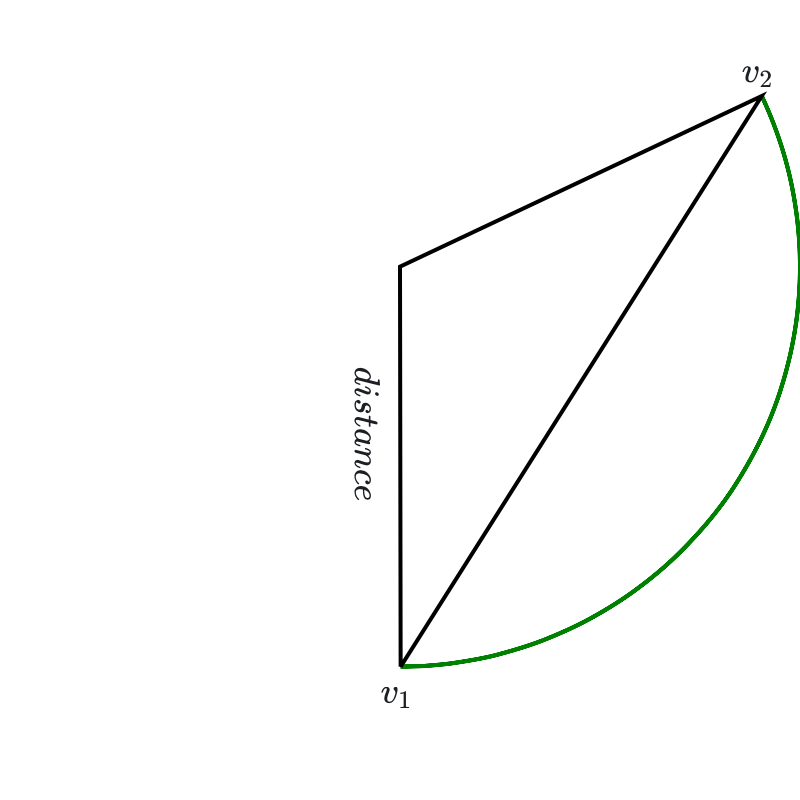
\includegraphics[width=3in,height=\textheight]{chapters/img/chord2.png}

}

\caption{\label{fig-chord}Chord of a circle}

\end{figure}

In algebraic terms, since \(D\) is the minimal value of \(\|v\|\) for
all \(v\in V\), we must have \(t(s)\ge D\).\\
On the other hand \[
\frac{d}{ds}\|t(s)\|^2 = \frac{d}{ds}(t(s)\cdot t(s)) =t(s)\cdot \frac{dt(s)}{ds} = t(s)\cdot(v_2-v_1).
\] Therefore \[
\frac{d}{ds}\|t(s)\|^2|_{s=0} = v_{1}\cdot(v_{2}-v_{1})=v_{1}\cdot v_{2}-\|v_{1}\|^2\le 0
\] since \(v_{1}\cdot v_{2}\le D^{2}\) and \(\|v_{1}\|^2=D^2\). If
\(v_{1}\cdot v_{2}<D^{2}\), then this derivative would be negative,
which would mean that there is a value of \(s\) where \(t(s)\) would be
less than \(D\). Since that can't happen, we conclude that
\(v_{1}\cdot v_{2}=D^{2}\) which means that \(v_{1}=v_{2}\) -- the
vectors have the same magnitude \(D\) and are parallel. This establishes
uniqueness.

\textbf{Note:} The essential ideas of this argument show that a compact
convex set in \(\mathbf{R}^{k}\) has a unique point closest to the
origin. The convex set in this instance, \[
V=\{p-q:p\in C(A^{+}),q\in C(A^{-})\},
\] is called the difference \(C(A^{+})-C(A^{-})\), and it is generally
true that the difference of convex sets is convex.

Now we can conclude this line of argument.

\textbf{Theorem:} Let \(p\) and \(q\) be points in \(C(A^{+})\) and
\(C(A^{-})\) respectively are such that \(\|p-q\|\) is minimal among all
such pairs. Let \(w=p-q\) and set \(B^{+}=w\cdot p\) and
\(B^{-}=w\cdot q\). Then \(f^{+}(x)=w\cdot x-B^{+}=0\) and
\(f^{-}(x)=w\cdot x-B^{-}\) are supporting hyperplanes for \(C(A^{+})\)
and \(C(A^{-})\) respectively and the associated margin \[
\tau_{w}(A^{+},A^{-})=\frac{B^{+}-B^{-}}{\|w\|} = \|p-q\|
\] is optimal.

\textbf{Proof:} First we show that \(f^{+}(x)=0\) is a supporting
hyperplane for \(C(A^{+})\). Suppose not. Then there is a point
\(p'\in C(A^{+})\) such that \(f^{+}(x)<0\). Consider the line segment
\(t(s) = (1-s)p+sp'\) running from \(p\) to \(p'\). By convexity it is
entirely contained in \(C(A^{+})\). Now look at the distance from points
on this segment to \(q\): \[
D(s)=\|t(s)-q\|^2.
\] We have \[
\frac{dD(s)}{ds}|_{s=0} = 2(p-q)\cdot (p'-p) = 2w\cdot (p'-p) = 2\left[(f^{+}(p')+B^{+})-(f^{+}(p)+B^{+})\right]
\] so \[
\frac{dD(s)}{ds}|_{s=0} = 2(f^{+}(p')-f^{+}(p))<0
\] since \(f(p)=0\). This means that \(D(s)\) is decreasing along
\(t(s)\) and so there is a point \(s'\) along \(t(s)\) where
\(\|t(s')-q\|<D\). This contradicts the fact that \(D\) is the minimal
distance. The same argument shows that \(f^{-}(x)=0\) is also a
supporting hyperplane.

Now the margin for this \(w\) is \[
\tau_{w}(A^{+},A^{-}) = \frac{w\cdot (p-q)}{\|w\|} = \|p-q\|=D
\] and as \(w\) varies we know this is the largest possible \(\tau\)
that can occur. Thus this is the maximal margin.

*Figure~\ref{fig-strict} shows how considering the closest point in the
convex hulls ``fixes'' the problem that we saw in
Figure~\ref{fig-nonstrict}. The closest point occurs at a point on the
boundary of the convex hull that is not one of the points in \(A^{+}\)
or \(A^{-}\).

\begin{figure}

{\centering 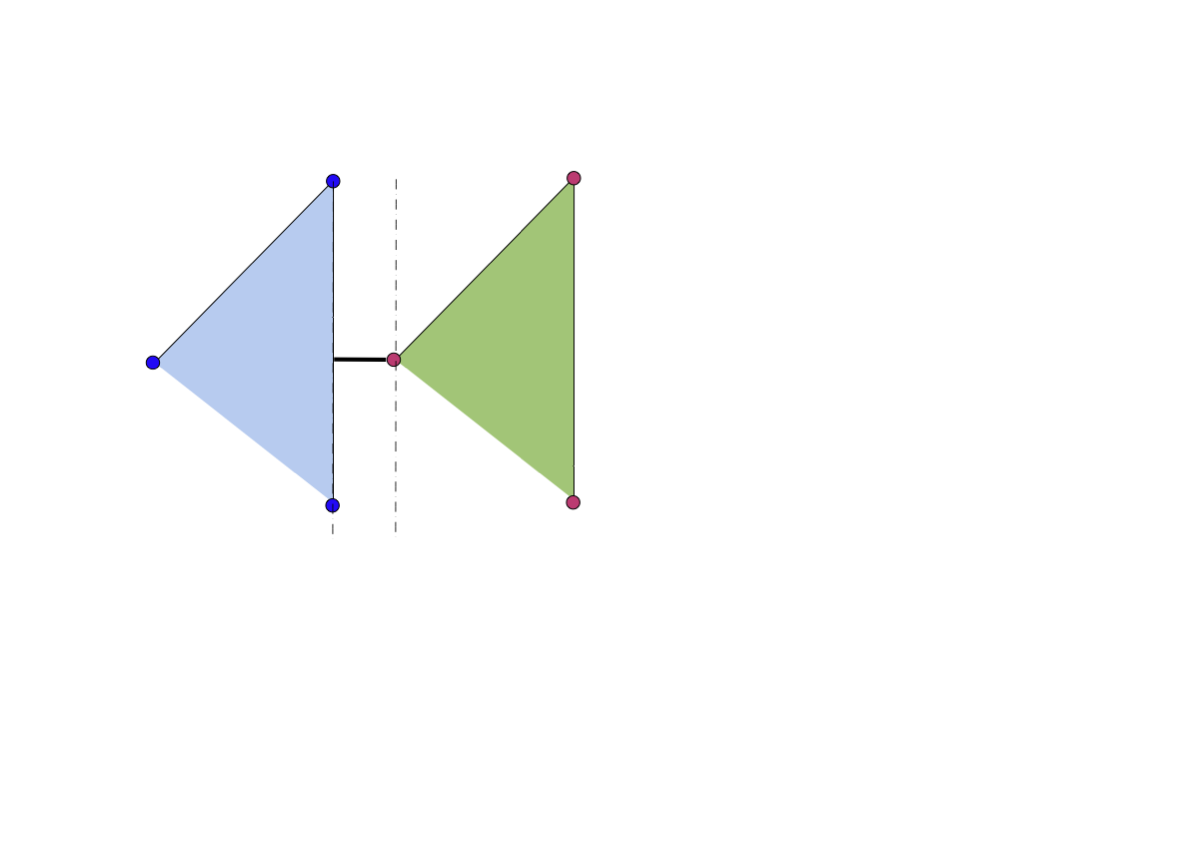
\includegraphics[width=0.5\textwidth,height=\textheight]{chapters/img/ConvexHullWithMargin.png}

}

\caption{\label{fig-strict}Closest distance between convex hulls gives
optimal margin}

\end{figure}

\hypertarget{finding-the-optimal-margin-classifier}{%
\section{Finding the Optimal Margin
Classifier}\label{finding-the-optimal-margin-classifier}}

Now that we have translated our problem into geometry, we can attempt to
develop an algorithm for solving it. To recap, we have two sets of
points \[
A^{+}=\{x^+_1,\ldots, x^+_{n_{+}}\}
\] and \[
A^{-}=\{x^-_1,\ldots, x^-_{n_{-}}\}
\] in \(\mathbf{R}^{k}\) that are linearly separable.

We wish to find points \(p\in C(A^{+})\) and \(q\in C(A^{-})\) such that
\[
\|p-q\|=\min_{p'\in C(A^{+}),q'\in C(A^{-})} \|p'-q'\|.
\]

Using the definition of the convex hull we can express this more
concretely. Since \(p\in C(A^{+})\), there are coefficients
\(\lambda^{+}_{i}\ge 0\) for \(i=1,\ldots,n_{+}\) and
\(\lambda^{-}_{i}\ge 0\) for \(i=1,\ldots, n_{-}\) so that \[
\begin{aligned}
p&=&\sum_{i=1}^{n_{+}}\lambda^{+}_{i} x^{+}_{i} \\
q&=&\sum_{i=1}^{n_{-}}\lambda^{-}_{i} x^{-}_{i} \\
\end{aligned}
\] where \(\sum_{i=1}^{n_{\pm}} \lambda_{i}^{\pm}=1\).

We can summarize this as follows:

\textbf{Optimization Problem 1:} Write
\(\lambda^{\pm}=(\lambda^{\pm}_{1},\ldots, \lambda^{\pm}_{n_{\pm}})\)
Define \[
w(\lambda^+,\lambda^-) = \sum_{i=1}^{n_{+}}\lambda^{+}_{i}x^{+}_{i} - \sum_{i=1}^{n_{-}}\lambda^{-}x^{-}_{i}
\] To find the supporting hyperplanes that define the optimal margin
between \(A^{+}\) and \(A^{-}\), find \(\lambda^{+}\) and
\(\lambda^{-}\) such that \(\|w(\lambda^{+},\lambda^{-})\|^2\) is
minimal among all such \(w\) where all \(\lambda^{\pm}_{i}\ge 0\) and
\(\sum_{i=1}^{n_{\pm}} \lambda^{\pm}_{i}=1\).

This is an example of a \emph{constrained optimization problem.} It's
worth observing that the \emph{objective function}
\(\|w(\lambda^{+},\lambda^{-})\|^2\) is just a quadratic function in the
\(\lambda^{\pm}.\) Indeed we can expand \[
\|w(\lambda^{+},\lambda^{-})\|^2 = (\sum_{i=1}^{n_{+}}\lambda^{+}_{i}x_{i}- \sum_{i=1}^{n_{-}}\lambda^{-}x^{-}_{i})\cdot(\sum_{i=1}^{n_{+}}\lambda^{+}_{i}x_{i}- \sum_{i=1}^{n_{-}}\lambda^{-}x^{-}_{i})
\] to obtain \[
\|w(\lambda^{+},\lambda^{-})\|^2 = R -2S +T
\] where \begin{equation}\protect\hypertarget{eq-kernel}{}{
\begin{aligned}
R &=& \sum_{i=1}^{n_{+}}\sum_{j=1}^{n_{+}}\lambda^{+}_{i}\lambda^{+}_{j}(x^{+}_{i}\cdot x^{+}_{j}) \\
S &=& \sum_{i=1}^{n_{+}}\sum_{j=1}^{n_{-}}\lambda^{+}_{i}\lambda^{-}_{j}(x^{+}_{i}\cdot x^{-}_{j}) \\
T &=& \sum_{i=1}^{n_{-}}\sum_{j=1}^{n_{-}}\lambda^{-}_{i}\lambda^{-}_{j}(x^{-}_{i}\cdot x^{-}_{j}) \\
\end{aligned}
}\label{eq-kernel}\end{equation} Thus the function we are trying to
minimize is relatively simple.

On the other hand, unlike optimization problems we have seen earlier in
these lectures, in which we can apply Lagrange multipliers, in this case
some of the constraints are inequalities -- namely the requirement that
all of the \(\lambda^{\pm}\ge 0\) -- rather than equalities. There is an
extensive theory of such problems that derives from the idea of Lagrange
multipliers. However, in these notes, we will not dive into that theory
but will instead construct an algorithm for solving the problem
directly.

\hypertarget{relaxing-the-constraints}{%
\subsection{Relaxing the constraints}\label{relaxing-the-constraints}}

Our first step in attacking this problem is to adjust our constraints
and our objective function slightly so that the problem becomes easier
to attack.

\textbf{Optimization Problem 2:} This is a slight revision of problem 1
above. We minimize: \[
Q(\lambda^{+},\lambda^{-}) = \|w(\lambda^{+},\lambda^{-})\|^2-\sum_{i=1}^{n_{+}}\lambda^{+}_{i}-\sum_{i=1}^{n_{-}}\lambda^{-}_{i}
\] subject to the constraints that all \(\lambda^{\pm}_{i}\ge 0\) and \[
\alpha = \sum_{i=1}^{n_{+}}\lambda^+_{i} = \sum_{i=1}^{n_{-}}\lambda^{-}_{i}.
\]

Problem 2 is like problem 1, except we don't require the sums of the
\(\lambda^{\pm}_{i}\) to be one, but only that they be equal to each
other; and we modify the objective function slightly. It turns out that
the solution to this optimization problem easily yields the solution to
our original one.

\textbf{Lemma:} Suppose \(\lambda^{+}\) and \(\lambda^{-}\) satisfy the
constraints of problem 2 and yield the minimal value for the objective
function \(Q(\lambda^{+},\lambda^{-})\). Then \(\alpha\not=0\). Rescale
the \(\lambda^{\pm}\) to have sum equal to one by dividing by
\(\alpha\), yielding \(\tau^{\pm}=(1/\alpha)\lambda^{\pm}\). Then
\(w(\tau^{+},\tau^{-})\) is a solution to optimization problem 1.

\textbf{Proof:} To show that \(\alpha\not=0\), suppose that
\(\lambda^{\pm}_{i}=0\) for all \(i\not=1\) and
\(\lambda=\lambda^{+}_{1}=\lambda^{-}_{1}\). The one-variable quadratic
function \(Q(\lambda)\) takes its minimum value at
\(\lambda=1/\|x_{1}^{+}-x_{1}^{-}\|^2\) and its value at that point is
negative. Therefore the minimum value of \(Q\) is negative, which means
\(\alpha\not=0\) at that minimum point.

For the equivalence, notice that \(\tau^{\pm}\) still satisfy the
constraints of problem 2. Therefore \[
Q(\lambda^{+},\lambda^{-}) = \|w(\lambda^{+},\lambda^{-})\|^2-2\alpha\le \|w(\tau^{+},\tau^{-})\|^2-2.
\] On the other hand, suppose that \(\sigma^{\pm}\) are a solution to
problem 1. Then \[
\|w(\sigma^{+},\sigma^{-})\|^2\le \|w(\tau^{+},\tau^{-})\|^2.
\] Therefore \[
\alpha^2 \|w(\sigma^{+},\sigma^{-})\|^2 = \|w(\alpha\sigma^{+},\alpha\sigma^{-})\|^2\le \|w(\lambda^{+},\lambda^{-})\|^2
\] and finally \[
\|w(\alpha\sigma^{+},\alpha\sigma^{-})\|^2-2\alpha\le Q(\lambda^{+},\lambda^{-})=\|w(\alpha\tau^{+},\alpha\tau^{-})\|^2-2\alpha.
\] Since \(Q\) is the minimal value, we have \[
\alpha^{2}\|w(\sigma^{+},\sigma^{-})\|^2 = \alpha^{2}\|w(\tau^{+},\tau^{-})\|^2
\] so that indeed \(w(\tau^{+},\tau^{-})\) gives a solution to Problem
1.

\hypertarget{sequential-minimal-optimization}{%
\subsection{Sequential Minimal
Optimization}\label{sequential-minimal-optimization}}

Now we outline an algorithm for solving Problem 2 that is called
Sequential Minimal Optimization that was introduced by John Platt in
1998 (See {[}10{]} and Chapter 12 of {[}11{]}). The algorithm is based
on the principle of ``gradient ascent'', where we exploit the fact that
the negative gradient of a function points in the direction of its most
rapid decrease and we take small steps in the direction of the negative
gradient until we reach the minimum.

However, in this case simplify this idea a little. Recall that the
objective function \(Q(\lambda^{+},\lambda^{-})\) is a quadratic
function in the \(\lambda\)'s and that we need to preserve the condition
that \(\sum \lambda^{+}_{i}=\sum\lambda^{-}_{i}\). So our approach is
going to be to take, one at a time, a pair \(\lambda^{+}_{i}\) and
\(\lambda^{-}_{j}\) and change them \emph{together} so that the equality
of the sums is preserved and the change reduces the value of the
objective function. Iterating this will take us to a minimum.

So, for example, let's look at \(\lambda^{+}_i\) and \(\lambda^{-}_{j}\)
and, for the moment, think of all of the other \(\lambda\)'s as
constants. Then our objective function reduces to a quadratic function
of these two variables that looks something like: \[
Q(\lambda_{i}^{+},\lambda_{j}^{-}) = a(\lambda^{+}_i)^2+b\lambda^{+}_i\lambda^{-}_j+c(\lambda^{-}_{i})^2+d\lambda^{+}_i+e\lambda^{-}_{j}+f.
\] The constraints that remain are \(\lambda^{\pm}\ge 0\), and we are
going to try to minimize \(Q\) by changing \(\lambda_{i}^{+}\) and
\(\lambda_{j}^{-}\) \emph{by the same amount} \(\delta\). Furthermore,
since we still must have \(\lambda_{i}^{+}+\delta\ge 0\) and
\(\lambda_{j}^{-}+\delta\ge 0\), we have

\begin{equation}\protect\hypertarget{eq-delta}{}{
\delta\ge M=\max\{-\lambda_{i}^{+},-\lambda_{j}^{-}\}
}\label{eq-delta}\end{equation}

In terms of this single variable \(\delta\), our optimization problem
becomes the job of finding the minimum of a quadratic polynomial in one
variable subject to the constraint in Equation~\ref{eq-delta}. This is
easy! There are two cases: the critical point of the quadratic is to the
left of \(M\), in which case the minimum value occurs at \(M\); or the
critical point of the quadratic is to the right of \(M\), in which case
the critical point occurs there. This is illustrated in
Figure~\ref{fig-quadratics}.

\begin{figure}

{\centering 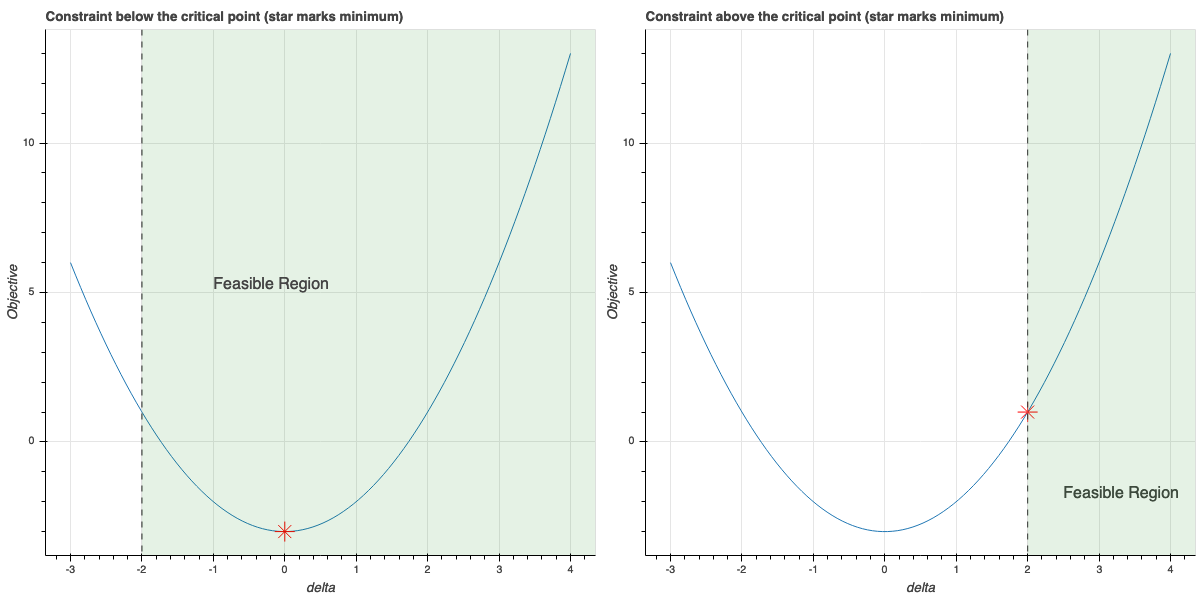
\includegraphics[width=0.5\textwidth,height=\textheight]{chapters/img/quadratic.png}

}

\caption{\label{fig-quadratics}Minimizing the 1-variable quadratic
objective function}

\end{figure}

Computationally, let's write \[
w_{\delta,i,j}(\lambda^{+},\lambda^{-}) = w(\lambda^{+},\lambda^{-})+\delta(x^{+}_{i}-x^{-}_{j}).
\] Then \[
\frac{d}{d\delta}(\|w_{\delta,i,j}(\lambda^{+},\lambda^{-})\|^2-2\alpha)  = 2w_{\delta,i,j}(\lambda^{+},\lambda^{-})\cdot(x^{+}_{i}-x^{-}_{j})-2
\] and using the definition of \(w_{\delta,i,j}\) we obtain the
following formula for the critical value of \(\delta\) by setting this
derivative to zero: \[
\delta_{i,j} = \frac{(1-w(\lambda^{+},\lambda^{-})\cdot(x_{i}^{+}-x_{j}^{-})}{\|x^+_{i}-x^{-}_{j}\|^2}
\]

Using this information we can describe the SMO algorithm.

\textbf{Algorithm (SMO, see {[}10{]}):}

\textbf{Given:} Two linearly separable sets of points
\(A^{+}=\{x_{1}^{+},\ldots,x_{n_{+}}^{+}\}\) and
\(A^{-}=\{x_{1}^{-},\ldots, x_{n_{-}}^{-}\}\) in \(\mathbf{R}^{k}\).

\textbf{Find:} Points \(p\) and \(q\) belonging to \(C(A^{+})\) and
\(C(A^{-})\) respectively such that \[
\|p-q\|^2=\min_{p'\in C(A^{+}),q'\in C(A^{-})} \|p'-q'\|^2
\]

\textbf{Initialization:} Set \(\lambda_{i}^{+}=\frac{1}{n_{+}}\) for
\(i=1,\ldots, n_{+}\) and \(\lambda_{i}^{-}=\frac{1}{n_{-}}\) for
\(i=1,\ldots, n_{-}\). Set \[
p(\lambda^{+})=\sum_{i=1}^{n_{+}}\lambda^{+}_{i}x^{+}_{i}
\] and \[
q(\lambda^{-})=\sum_{i=1}^{n_{-}}\lambda^{-}_{i}x^{-}_{i}
\] Notice that
\(w(\lambda^{+},\lambda^{-})=p(\lambda^{+})-q(\lambda^{-})\). Let
\(\alpha=\sum_{i=1}^{n_{+}}\lambda^{+}=\sum_{i=1}^{n_{-}}\lambda^{-}\).
These sums will remain equal to each other throughout the operation of
the algorithm.

Repeat the following steps until maximum value of \(\delta^{*}\)
computed in each iteration is smaller than some tolerance (so that the
change in all of the \(\lambda\)'s is very small):

\begin{itemize}
\tightlist
\item
  For each pair \(i,j\) with \(1\le i\le n_{+}\) and
  \(1\le j\le n_{-}\), compute \[
  M_{i,j} = \max\{-\lambda_{i}^{+},-\lambda_{j}^{-}\}
  \] and \[
  \delta_{i,j} = \frac{1-(p(\lambda^{+})-q(\lambda^{-}))\cdot(x_{i}^{+}-x_{j}^{-})}{\|x^+_{i}-x^{-}_{j}\|^2}.
  \] If \(\delta_{i,j}\ge M\) then set \(\delta^{*}=\delta_{i,j}\);
  otherwise set \(\delta^{*}=M\). Then update the \(\lambda^{\pm}\) by
  the equations: \[
  \begin{aligned}
  \lambda^{+}_{i}&=&\lambda^{+}_{i}+\delta_{i,j}^{*} \\
  \lambda^{+}_{j}&=&\lambda^{-}_{j}+\delta_{i,j}^{*} \\
  \end{aligned}
  \]
\end{itemize}

When this algorithm finishes, \(p\approx p(\lambda^{+})\) and
\(q\approx q(\lambda^{-})\) will be very good approximations to the
desired closest points.

Recall that if we set \(w=p-q\), then the optimal margin classifier is

\[
f(x)=w\cdot x - \frac{B^{+}+B^{-}}{2}=0
\]

where \(B^{+}=w\cdot p\) and \(B^{-}=w\cdot q\). Since \(w=p-q\) we can
simplify this to obtain

\[
f(x)=(p-q)\cdot x -\frac{\|p\|^2-\|q\|^2}{2}=0.
\]

In Figure~\ref{fig-penguinsolution}, we show the result of applying this
algorithm to the penguin data and illustrate the closest points as found
by an implementation of the SMO algorithm, together with the optimal
classifying line.

Bearing in mind that the y-axis is scaled by a factor of 200, we obtain
the following rule for distinguishing between Adelie and Gentoo penguins
-- if the culmen depth and body mass put you above the red line, you are
a Gentoo penguin, otherwise you are an Adelie.

\begin{figure}

{\centering 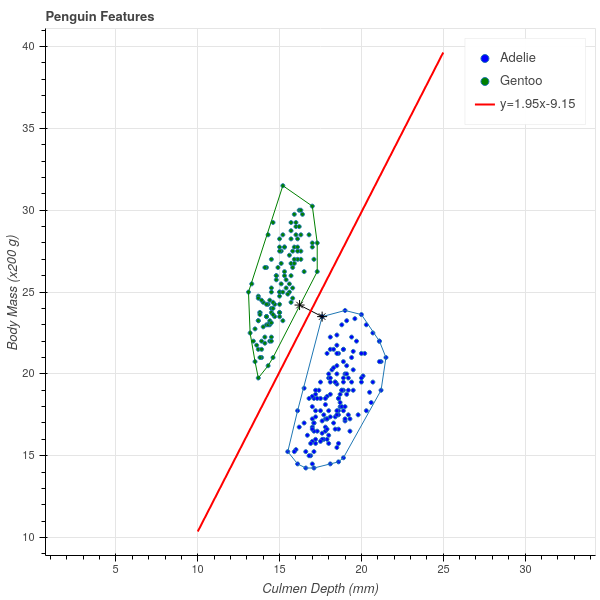
\includegraphics[width=0.5\textwidth,height=\textheight]{chapters/img/solution.png}

}

\caption{\label{fig-penguinsolution}Closest points in convex hulls of
penguin data}

\end{figure}

\hypertarget{inseparable-sets}{%
\section{Inseparable Sets}\label{inseparable-sets}}

Not surprisingly, real life is often more complicated than the penguin
example we've discussed at length in these notes. In particular,
sometimes we have to work with sets that are not linearly separable.
Instead, we might have two point clouds, the bulk of which are
separable, but because of some outliers there is no hyperplane we can
draw that separates the two sets into two halfplanes.

Fortunately, all is not lost. There are two common ways to address this
problem, and while we won't take the time to develop the theory behind
them, we can at least outline how they work.

\hypertarget{best-separating-hyperplanes}{%
\subsection{Best Separating
Hyperplanes}\label{best-separating-hyperplanes}}

If our sets are not linearly separable, then their convex hulls overlap
and so our technique for finding the closest points of the convex hulls
won't work. In this case, we can ``shrink'' the convex hull by
considering combinations of points \(\sum_{i}\lambda_{i}x_{i}\) where
\(\sum\lambda_{i}=1\) and \(C\ge\lambda_{i}\ge 0\) for some \(C\le 1\).
For \(C\) small enough, reduced convex hulls will be linearly separable
-- although some outlier points from each class will lie outside of them
-- and we can find hyperplane that separates the reduced hulls.\\
In practice, this means we allow a few points to lie on the ``wrong
side'' of the hyperplane. Our tolerance for these mistakes depends on
\(C\), but we can include \(C\) in the optimization problem to try to
find the smallest \(C\) that ``works''.

\hypertarget{nonlinear-kernels}{%
\subsection{Nonlinear kernels}\label{nonlinear-kernels}}

The second option is to look not for separating hyperplanes but instead
for separating curves -- perhaps polynomials or even more exotic curves.
This can be achieved by taking advantage of the form of
Equation~\ref{eq-kernel}. As you see there, the only way the points
\(x_{i}^{\pm}\) enter in to the function being minimized is through the
inner products \(x_{i}^{\pm}\cdot x_{j}^{\pm}\). We can adopt a
different inner product than the usual Euclidean one, and reconsider the
problem using this different inner product. This amounts to embedding
our points in a higher dimensional space where they are more likely to
be linearly separable. Again, we will not pursue the mathematics of this
further in these notes.

\hypertarget{sec-exercises}{%
\section{Exercises}\label{sec-exercises}}

\begin{enumerate}
\def\labelenumi{\arabic{enumi}.}
\item
  Prove that, if \(f(x)=w\cdot x+b=0\) is a hyperplane in
  \(\mathbf{R}^{k}\), then the two ``sides'' of this hyperplane,
  consisting of the points where \(f(x)\ge 0\) and \(f(x)\le 0\), are
  both convex sets.
\item
  Prove that \(C(S)\) is the intersection of all the halfplanes
  \(f(x)\ge 0\) as \(f(x)=w\cdot x+b\) runs through all supporting
  hyperplanes for \(S\) where \(f(x)\ge 0\) for all \(p\in S\).
\item
  Prove that \(C(S)\) is bounded. Hint: show that \(S\) is contained in
  a sphere of sufficiently large radius centered at zero, and then that
  \(C(S)\) is contained in that sphere as well.
\item
  Confirm the final formula for the optimal margin classifier at the end
  of the lecture.
\end{enumerate}

\bookmarksetup{startatroot}

\hypertarget{references}{%
\chapter*{References}\label{references}}
\addcontentsline{toc}{chapter}{References}

\markboth{References}{References}

\hypertarget{refs}{}
\begin{CSLReferences}{0}{0}
\leavevmode\vadjust pre{\hypertarget{ref-irvine}{}}%
\CSLLeftMargin{{[}1{]} }%
\CSLRightInline{\textsc{U.C. Irvine ML Repository}. {Auto MPG
Dataset}.Available at
\url{http://https://archive.ics.uci.edu/ml/datasets/Auto+MPG}.}

\leavevmode\vadjust pre{\hypertarget{ref-Bertsekas}{}}%
\CSLLeftMargin{{[}2{]} }%
\CSLRightInline{\textsc{Bertsekas}, D. P. and \textsc{Tsitsiklis}, J. N.
(2008). \emph{Introduction to probability}. Athena Scientific.}

\leavevmode\vadjust pre{\hypertarget{ref-sentences}{}}%
\CSLLeftMargin{{[}3{]} }%
\CSLRightInline{\textsc{U.C. Irvine ML Repository}. {Sentiment Labelled
Sentences Data Set}.Available at
\url{https://archive.ics.uci.edu/ml/datasets/Sentiment+Labelled+Sentences}.}

\leavevmode\vadjust pre{\hypertarget{ref-KaggleFoodData}{}}%
\CSLLeftMargin{{[}4{]} }%
\CSLRightInline{\textsc{Jack Daoud}. {Marketing Analytics}.Available at
\url{https://www.kaggle.com/datasets/jackdaoud/marketing-data}.}

\leavevmode\vadjust pre{\hypertarget{ref-MNISTDatabase}{}}%
\CSLLeftMargin{{[}5{]} }%
\CSLRightInline{\textsc{LeCun}, Y., \textsc{Cortes}, C. and
\textsc{Burges}, C. {The MNIST Database}.Available at
\url{http://yann.lecun.com/exdb/mnist/}.}

\leavevmode\vadjust pre{\hypertarget{ref-vapnik92}{}}%
\CSLLeftMargin{{[}6{]} }%
\CSLRightInline{\textsc{Boser}, B., \textsc{Guyon}, I. and
\textsc{Vapnik}, V.
\href{https://dl.acm.org/doi/pdf/10.1145/130385.130401}{{A training
algorithm for optimal margin classifiers}}. In \emph{Colt '92:
Proceedings of the fifth annual workshop on computational learning
theory} (D. Haussler, ed) pp 144--52. ACM.}

\leavevmode\vadjust pre{\hypertarget{ref-bennettDuality}{}}%
\CSLLeftMargin{{[}7{]} }%
\CSLRightInline{\textsc{Bennett}, K. P. and \textsc{Bredensteiner}, E.
J. (2000). Duality and geometry in SVM classifiers. In \emph{Proceedings
of the seventeenth international conference on machine learning} (P.
Langley, ed). Morgan Kaufmann Publishers.}

\leavevmode\vadjust pre{\hypertarget{ref-penguins}{}}%
\CSLLeftMargin{{[}8{]} }%
\CSLRightInline{\textsc{Gorman}, K. B., \textsc{Williams}, T. D. and
\textsc{Fraser}, W. R. (2014).
\href{https://doi.org/10.1371/journal.pone.0090081}{Ecological sexual
dimorphism and environmental variability within a community of antarctic
penguins (genus pygoscelis)}. \emph{PLoS ONE} \textbf{9(3)} --13.}

\leavevmode\vadjust pre{\hypertarget{ref-penguindata}{}}%
\CSLLeftMargin{{[}9{]} }%
\CSLRightInline{\textsc{Horst}, A. Palmer penguins.Available at
\url{https://github.com/allisonhorst/palmerpenguins}.}

\leavevmode\vadjust pre{\hypertarget{ref-plattSMO}{}}%
\CSLLeftMargin{{[}10{]} }%
\CSLRightInline{\textsc{Platt}, J. C. (1998).
\emph{\href{https://www-ai.cs.tu-dortmund.de/LEHRE/SEMINARE/SS09/AKTARBEITENDESDM/LITERATUR/PlattSMO.pdf}{Sequential
minimal optimization: A fast algorithm for training support vector
machines}}. Microsoft Research.}

\leavevmode\vadjust pre{\hypertarget{ref-KernelMethodAdvances}{}}%
\CSLLeftMargin{{[}11{]} }%
\CSLRightInline{\textsc{Schölkopf}, B., \textsc{Burges}, C. and
\textsc{Smola}, A. (1998). \emph{Advances in kernel methods: Support
vector learning}. MIT Press.}

\end{CSLReferences}


\backmatter

\end{document}
